%! TEX program = xelatex
% ============================================================
%  PLANTILLA BASE — · Ing. de Sistemas
%  Compilar:  xelatex → bibtex → xelatex → xelatex
% ============================================================

\documentclass[11pt, a4paper, oneside]{report}

% ── Fuentes y codificación ───────────────────────────────
\usepackage{fontspec}
\setmainfont{Times New Roman}
\setmonofont{Consolas}
\usepackage{babel}
\babelprovide[import, main]{spanish}
\usepackage{tabularx}
\usepackage{hyperref}
\usepackage{pdflscape}
\usepackage{lscape}
\usepackage{tikz}
% ── Márgenes ────────────────────────────────────────────
\usepackage{geometry}
\geometry{
  top    = 2.54cm,
  bottom = 2.54cm,
  left   = 3.00cm,
  right  = 2.54cm,
}
\setlength{\headheight}{14.5pt}

% ── Interlineado y párrafo ───────────────────────────────
\usepackage{setspace}
\setstretch{1.5}
\usepackage{parskip}
\setlength{\parskip}{4pt plus 1pt}
\setlength{\parindent}{1.25cm}

% ── Figuras y tablas ────────────────────────────────────
\usepackage{float}

% ── Colores UPeU ────────────────────────────────────────
\usepackage[table]{xcolor}
\definecolor{upeu_dark}{HTML}{1A3A6B}
\definecolor{upeu_mid}{HTML}{2E75B6}
\definecolor{upeu_light}{HTML}{D6E4F0}
\definecolor{upeu_gold}{HTML}{B8860B}
\definecolor{body_gray}{HTML}{404040}
\definecolor{hint_gray}{HTML}{9E9E9E}
\definecolor{diag_bg}{HTML}{0D1117}
\definecolor{sev_critico}{HTML}{C0392B}
\definecolor{sev_alto}{HTML}{E67E22}
\definecolor{sev_medio}{HTML}{F1C40F}
\definecolor{sev_bajo}{HTML}{27AE60}

% ── Encabezado y pie ────────────────────────────────────
\usepackage{fancyhdr}
\pagestyle{fancy}
\fancyhf{}
\fancyhead[R]{%
  {\color{body_gray}\small\itshape }%
  {\color{upeu_dark}\small\bfseries Ingeniería de Sistemas · UPeU}%
}
\renewcommand{\headrule}{{\color{upeu_mid}\rule{\headwidth}{0.8pt}}}
\fancyfoot[L]{\scriptsize\textcolor{upeu_mid}{E1 -- Levantamiento, Topología y Segmentación de Red · Franco's SAC}}
\fancyfoot[R]{{\color{body_gray}\small Página \thepage}}
\renewcommand{\footrule}{{\color{upeu_mid}\rule{\headwidth}{0.8pt}}}

% PARCHE: Obliga a todas las páginas (incluyendo capítulos e índice) a ser Fancy
\makeatletter
\let\ps@plain\ps@fancy
\makeatother

% ── Títulos / secciones ──────────────────────────────────
\usepackage{titlesec}

% Capitulo  (Heading 1)
\titleformat{\chapter}[display]
  {\normalfont\centering}
  {\color{upeu_mid}\bfseries\fontsize{13}{17}\selectfont CAPÍTULO \thechapter}
  {6pt}
  {\color{upeu_dark}\bfseries\fontsize{20}{26}\selectfont}
  [\vspace{6pt}\textcolor{upeu_mid}{\rule{\textwidth}{1.2pt}}]

\titlespacing{\chapter}{0pt}{28pt}{16pt}

% Seccion  (Heading 2)
\titleformat{\section}[hang]
  {\normalfont\bfseries\large\color{upeu_dark}}
  {\thesection}{0.7em}{}
\titlespacing{\section}{0pt}{14pt}{6pt}

% Subseccion  (Heading 3)
\titleformat{\subsection}[hang]
  {\normalfont\bfseries\normalsize\color{upeu_mid}\itshape}
  {\thesubsection}{0.7em}{}
\titlespacing{\subsection}{0pt}{10pt}{4pt}

% Sub-subseccion  (Heading 4)
\titleformat{\subsubsection}[hang]
  {\normalfont\bfseries\normalsize\color{body_gray}}
  {\thesubsubsection}{0.7em}{}
\titlespacing{\subsubsection}{0pt}{8pt}{2pt}

\setcounter{secnumdepth}{3}
\setcounter{tocdepth}{3}

% ── Índice: forzar mismo formato que \chapter ────────────
% FIX: \contentsname usa \chapter* internamente, lo que omite
%      el \titleformat definido arriba. Con \addtocontents y
%      \renewcommand forzamos el título con el estilo correcto.
\usepackage{tocloft}
\renewcommand{\cfttoctitlefont}{\normalfont\bfseries\Large\color{upeu_dark}}
\renewcommand{\cftaftertoctitle}{%
}
\setlength{\cftbeforetoctitleskip}{10pt}
\setlength{\cftaftertoctitleskip}{16pt}

\renewcommand{\cftchapfont}{\bfseries\color{upeu_dark}}
\renewcommand{\cftsecfont}{\color{body_gray}}
\renewcommand{\cftsubsecfont}{\small\color{body_gray}}
\renewcommand{\cftchapleader}{\cftdotfill{\cftdotsep}}
\renewcommand{\cftsecleader}{\cftdotfill{\cftdotsep}}

% ── Graficos ────────────────────────────────────────────
\usepackage{graphicx}
\graphicspath{{./img/}{./}}
\usepackage{chngcntr}
\counterwithout{figure}{chapter}
\counterwithout{table}{chapter}  % por si acaso también para tablas

% ── Tablas ──────────────────────────────────────────────
\usepackage{booktabs}
\usepackage{tabularx}
\usepackage{xltabular}
\usepackage{array}
\newcolumntype{L}[1]{>{\raggedright\arraybackslash}p{#1}}
\newcolumntype{C}[1]{>{\centering\arraybackslash}p{#1}}
% Columnas con centrado vertical
\newcolumntype{M}[1]{>{\raggedright\arraybackslash}m{#1}}
\newcolumntype{N}[1]{>{\centering\arraybackslash}m{#1}}

% ── Listas ──────────────────────────────────────────────
\usepackage{enumitem}
\setlist{noitemsep, topsep=4pt}

% ── Citas IEEE ──────────────────────────────────────────
\usepackage[numbers]{natbib}
\bibliographystyle{ieeetr}

% ── Hipervinculos ────────────────────────────────────────
\usepackage{hyperref}
\hypersetup{
  colorlinks = true,
  linkcolor  = upeu_dark,
  urlcolor   = upeu_mid,
  citecolor  = upeu_mid,
  pdftitle   = {E1 -- Levantamiento, Topologia y Segmentacion de Red -- Franco's SAC -- ITI UPeU 2026},
  pdfauthor  = {Salazar Tocas, Ruben Mark; Sauñe Fernandez, Uziel Elias},
}

% ── Captions ────────────────────────────────────────────
\usepackage{caption}
\captionsetup{
  font      = small,
  labelfont = {bf, color=upeu_dark},
  textfont  = {color=body_gray},
  skip      = 4pt,
  labelsep  = period
}

\addto\captionsspanish{%
  \renewcommand{\tablename}{Tabla}%
  \renewcommand{\figurename}{Figura}%
}

% ── Codigo fuente ────────────────────────────────────────
\usepackage{listings}
\lstset{
  basicstyle   = \ttfamily\small,
  keywordstyle = \bfseries\color{upeu_dark},
  commentstyle = \itshape\color{hint_gray},
  stringstyle  = \color{upeu_mid},
  frame        = single,
  rulecolor    = \color{upeu_mid},
  breaklines   = true,
  numbers      = left,
  numberstyle  = \tiny\color{hint_gray},
}

\usepackage{microtype}
\usepackage{amsmath}

% ── Estilo para diagramas ASCII (fondo oscuro, Consolas) ────
\lstdefinestyle{diagrama}{
  basicstyle    = {\ttfamily\scriptsize\color[HTML]{E6EDF3}},
  backgroundcolor = \color{diag_bg},
  frame         = single,
  rulecolor     = \color{diag_bg},
  numbers       = none,
  breaklines    = false,
  keepspaces    = true,
}

% ── Caja de nota / info-box ──────────────────────────────────
\newsavebox{\notaboxsb}
\newenvironment{notabox}[1]{%
  \begin{lrbox}{\notaboxsb}%
  \begin{minipage}{\dimexpr\textwidth-2\fboxsep\relax}%
  \vspace{4pt}\textcolor{upeu_dark}{\textbf{#1}}\\[2pt]\small%
}{%
  \vspace{4pt}%
  \end{minipage}%
  \end{lrbox}%
  \vspace{6pt}\par\noindent\colorbox{upeu_light}{\usebox{\notaboxsb}}\par\vspace{6pt}%
}

% ── Espaciado floats y paginación ────────────────────────────
\setlength{\textfloatsep}{10pt plus 2pt minus 4pt}
\setlength{\floatsep}{6pt plus 2pt minus 2pt}
\setlength{\intextsep}{8pt plus 2pt minus 2pt}
\setlength{\abovecaptionskip}{4pt}
\setlength{\belowcaptionskip}{2pt}
\raggedbottom
% ============================================================
\begin{document}
\widowpenalty=10000
\clubpenalty=10000
\displaywidowpenalty=10000
% ============================================================

% ── PORTADA ─────────────────────────────────────────────────
\begin{titlepage}
  \pagestyle{empty}
  \centering

  \vspace*{\fill}

  {\color{upeu_dark}\bfseries\Large UNIVERSIDAD PERUANA UNIÓN}\\[5pt]
  {\color{body_gray}\large Facultad de Ingeniería y Arquitectura}\\[3pt]
  {\color{body_gray}\normalsize Escuela Profesional de Ingeniería de Sistemas}

  \vspace{12pt}

  
\includegraphics[width=6.5cm]{img/logo-upeu.png}\\[10pt]

  % ── Nombre del proyecto ──
  {\color{upeu_mid}\bfseries\normalsize CE031}\\
  {\color{upeu_dark}\bfseries\large Entregable 1: Diseño de Red}\\[4pt]

  \vspace{0.3cm}

  % ── Curso y Docente ──
  \begin{tabular}{@{}ll@{}}
    {\color{upeu_dark}\bfseries Área:}    & {\color{body_gray} Infraestructura Tecnologica} \\[4pt]
    {\color{upeu_dark}\bfseries Asesor:} & {\color{body_gray} Mg. Fernando Asin} \\
  \end{tabular}

  \vspace{0.3cm}

  {\color{upeu_dark}\bfseries Integrantes:}\\[6pt]

  \begin{tabular}{@{}|l|@{}}
    \arrayrulecolor{upeu_dark}
    \rowcolor{upeu_dark}
    {\color{white}\bfseries\small Integrante} \\ \hline
    {\color{body_gray}\small Salazar Tocas, Rubén Mark} \\ \hline
    {\color{body_gray}\small Chavarri Centeno, Jorge Andrés} \\ \hline
    {\color{body_gray}\small Sauñe Fernandez, Uziel Elias} \\ \hline
    {\color{body_gray}\small Pedraza Perez, Joshua Josue} \\ \hline
    {\color{body_gray}\small Lanche Cerro, Hilter Piero} \\ \hline
    {\color{body_gray}\small Rivera Matías, Joel Joshep} \\ \hline
    {\color{body_gray}\small Evan Chacon} \\ \hline
    {\color{body_gray}\small Ramos Turpo, Roxwell Jesus} \\ \hline
    {\color{body_gray}\small Vallejos Cotrina, Pamela} \\ \hline
    {\color{body_gray}\small Vergara, Verónica Lisseth} \\ \hline
  \end{tabular}

  \vspace{0.6cm}
  {\color{body_gray} Junio, 2026}

  \vspace*{\fill}

\end{titlepage}

% ── CONTROL DE VERSIONES ────────────────────────────────────
\newpage

\thispagestyle{empty}
\vspace{2cm}

{\centering
% {\color{upeu_dark}\bfseries\Large Control de Versiones}\\[0.4cm]

\begin{tabular}{@{}|C{1.5cm}|C{2.2cm}|L{3cm}|L{5cm}|C{2cm}|@{}}

  \arrayrulecolor{upeu_dark}

  \rowcolor{upeu_dark}
  {\color{white}\bfseries\small Versión} &
  {\color{white}\bfseries\small Fecha} &
  {\color{white}\bfseries\small Autor} &
  {\color{white}\bfseries\small Descripción} &
  {\color{white}\bfseries\small Estado} \\  \hline

  \small v1.0 & \small 10/05/2026 & \small Salazar Tocas, R.M. & \small Creación inicial del documento & \small Borrador \\ \hline
  \small v1.1 & \small 18/05/2026 & \small Sauñe Fernandez, U.  & \small Reqs técnicos RT-01..RT-17 completos & \small Revisión \\ \hline
  \small v1.2 & \small 01/06/2026 & \small Salazar Tocas, R.M. & \small Topología y vSwitches H1-H5 & \small Revisión \\ \hline
  \small v1.3 & \small 15/06/2026 & \small Salazar Tocas, R.M. & \small Eliminación H4 Backup Crítico; renumeración a 5 hipervisores & \small Revisión \\ \hline
  \small v1.4 & \small 23/06/2026 & \small Salazar Tocas, R.M. & \small Consolidación AWS DR; versión final E1 & \small Aprobado \\ \hline

\end{tabular}
\par}

% ── INDICE ──────────────────────────────────────────────────
\newpage
\pagestyle{fancy}
\pagenumbering{roman}
\tableofcontents
% \listoffigures    % descomenta si usas figuras
% \listoftables     % descomenta si usas tablas
\clearpage
\pagenumbering{arabic}

% ============================================================
% EMPIEZA LA REDACCION
% ============================================================

\newpage
\pagestyle{fancy} % Esto lo vuelve a activar para el Capítulo 1 en adelante

% ── RESUMEN EJECUTIVO ───────────────────────────────────────────
\chapter{Resumen Ejecutivo}
\section{Problema organizacional identificado}
Franco's SAC presenta una brecha tecnológica significativa debido a la ausencia de una infraestructura formal de red, servidores y servicios tecnológicos centralizados. Actualmente, la empresa opera con recursos informáticos limitados, una red inalámbrica sin segmentación, pocos equipos de cómputo activos y sin mecanismos adecuados de seguridad, respaldo o monitoreo.

Asimismo, la organización no cuenta con un sistema ERP que integre sus procesos de ventas, inventario, producción y administración. Esta situación ocasiona que gran parte de la información sea gestionada de forma manual o mediante hojas de cálculo, generando riesgos de duplicidad, errores operativos, pérdida de información y baja trazabilidad.

Otro problema relevante es la falta de conectividad entre sus tres locales operativos, lo cual impide el intercambio de información en tiempo real entre la sede administrativa, ventas, inventario y las plantas de producción. En consecuencia, la empresa no dispone de una base tecnológica sólida que permita sostener su crecimiento, mejorar la toma de decisiones y avanzar hacia un proceso de transformación digital.
\section{Objetivo general de sistema}
Diseñar una infraestructura tecnológica segura, segmentada, escalable e híbrida para Franco's SAC, que permita interconectar sus tres locales operativos, soportar la futura implementación de un sistema ERP, centralizar servicios críticos, proteger la información organizacional y garantizar la disponibilidad de los procesos principales de ventas, inventario, producción y administración.
\section{Alcance del proyecto (incluye / no incluye)}
El alcance del proyecto comprende el levantamiento de requerimientos técnicos y de negocio para el diseño de una infraestructura tecnológica orientada a Franco's SAC. La propuesta incluye el diseño de una red segmentada mediante VLANs, direccionamiento IP estructurado, conectividad segura entre locales mediante VPN, firewall perimetral con pfSense, virtualización sobre VMware ESXi, servicios de autenticación, soporte para microservicios contenerizados, zona DMZ, WAF, monitoreo centralizado y respaldo de información.

También se considera una arquitectura híbrida con integración a servicios cloud, permitiendo complementar la infraestructura local con servicios como almacenamiento, publicación de aplicaciones, respaldo y monitoreo externo. La solución será diseñada para soportar aproximadamente entre 30 y 40 usuarios distribuidos en las áreas de administración, ventas, inventario y producción.

El proyecto no contempla la compra real de hardware para la empresa, la implementación física definitiva en las instalaciones de Franco's SAC ni la operación productiva real de la solución. La implementación se plantea dentro del entorno académico y de laboratorio, utilizando los recursos disponibles en la Universidad Peruana Unión para simular el escenario tecnológico de la organización.
\section{Stakeholders}
Los principales stakeholders del proyecto son aquellos actores que participan, se benefician o se ven impactados por el diseño de la infraestructura tecnológica propuesta para Franco's SAC.

\begin{table}[htbp]
\centering
\caption{Stakeholders del proyecto}
\small
\renewcommand{\arraystretch}{1.25}
\begin{tabularx}{\textwidth}{|L{3.5cm}|X|}
\hline
\rowcolor{upeu_light}
\textbf{Stakeholder} & \textbf{Interés dentro del proyecto} \\
\hline
Dirección de Franco's SAC & Mejorar la gestión general del negocio mediante una infraestructura tecnológica que permita mayor control, disponibilidad de información y soporte para la transformación digital. \\
\hline
Área de Administración & Contar con acceso seguro y centralizado a la información financiera, contable, de recursos humanos y de gestión interna. \\
\hline
Área de Ventas & Disponer de conectividad y servicios tecnológicos que permitan registrar pedidos, facturación y atención a clientes de manera integrada. \\
\hline
Área de Inventario & Mejorar el control de stock de insumos y productos terminados mediante sistemas conectados y disponibilidad de información actualizada. \\
\hline
Área de Producción & Integrar las plantas de producción con la sede central para registrar y consultar información operativa en tiempo real. \\
\hline
Equipo de Infraestructura TI & Diseñar la red, servidores, seguridad, conectividad, servicios internos, monitoreo y respaldo de la solución propuesta. \\
\hline
Área de Desarrollo & Contar con una base tecnológica adecuada para desplegar el sistema ERP basado en microservicios, contenedores y bases de datos. \\
\hline
Asesor y docentes evaluadores & Validar el cumplimiento técnico, metodológico y académico del proyecto dentro de la línea de Infraestructura Tecnológica. \\
\hline
Usuarios finales & Utilizar los servicios tecnológicos de forma segura, disponible y acorde con sus funciones dentro de la empresa. \\
\hline
\end{tabularx}
\end{table}
\section{Beneficio esperado}
El beneficio esperado del proyecto es proporcionar a Franco's SAC una base tecnológica sólida que permita mejorar la continuidad operativa, la seguridad de la información y la integración de sus procesos principales. Con la infraestructura propuesta, la empresa podrá contar con conectividad segura entre sus tres locales, segmentación de red por áreas, servicios centralizados, respaldo de información, monitoreo de disponibilidad y soporte para la implementación futura de un sistema ERP.
La solución permitirá reducir los riesgos asociados a la gestión manual de información, mejorar el control de ventas, inventario y producción, facilitar la toma de decisiones y fortalecer la protección de los datos organizacionales. De esta manera, el proyecto contribuye directamente al proceso de transformación digital de Franco's SAC, alineando la infraestructura tecnológica con sus necesidades actuales y su crecimiento futuro.

% ── CE0311 ──────────────────────────────────────────────────
\chapter{CE0311 - Levantamiento de Requerimientos Tecnicos y de Negocio}

\section{Contexto de la organización}

Franco's SAC es una empresa peruana perteneciente al sector agroindustrial alimentario, dedicada a la fabricación y comercialización de snacks naturales. Su operación se encuentra distribuida en tres locales, los cuales cumplen funciones diferenciadas dentro de la organización: producción, administración, ventas, inventario y una segunda planta de producción.

De acuerdo con el levantamiento realizado, la empresa cuenta aproximadamente con entre 30 y 40 trabajadores distribuidos en sus diferentes áreas operativas. Esta estructura evidencia la necesidad de contar con una infraestructura tecnológica que permita integrar la información generada por cada área, mejorar la comunicación entre sedes y brindar soporte a los procesos principales del negocio.

La organización tiene como misión producir y comercializar snacks de alta calidad utilizando ingredientes frescos y naturales, buscando satisfacer las necesidades de sus clientes mediante productos diferenciados por su sabor y frescura. Asimismo, su visión se orienta a ser reconocida a nivel nacional e internacional por la excelencia de sus productos, la calidad de sus procesos y su compromiso con una producción responsable y sostenible.

\begin{table}[htbp]
\centering
\caption{Áreas funcionales de Franco's SAC}
\small
\renewcommand{\arraystretch}{1.25}
\begin{tabularx}{\textwidth}{|M{3.2cm}|X|L{3cm}|N{1.8cm}|}
\hline
\rowcolor{upeu_light}
\textbf{Área} & \textbf{Función principal} & \textbf{Local} & \textbf{Usuarios aprox.} \\
\hline
Administración & Gestión financiera, contabilidad, recursos humanos y dirección general. & Local 2 -- Sede Central & 5 -- 8 \\
\hline
Ventas & Atención a clientes, facturación, registro de pedidos y distribución. & Local 2 -- Sede Central & 8 -- 12 \\
\hline
Inventario & Control de stock de insumos y productos terminados. & Local 2 -- Sede Central & 3 -- 5 \\
\hline
Producción & Fabricación de snacks, control de calidad y empaque. & Local 1 & 15 -- 20 \\
\hline
Producción L3 & Segunda planta de fabricación y empaque orientada a la expansión productiva. & Local 3 & Estimado 15 -- 20 \\
\hline
\end{tabularx}
\end{table}

\section{Diagnóstico de la infraestructura actual AS-IS}
Durante el levantamiento inicial se identificó que Franco's SAC no cuenta con una infraestructura tecnológica formalmente estructurada. La operación diaria se sostiene con recursos limitados, principalmente equipos de cómputo aislados, conectividad inalámbrica básica y procesos administrativos gestionados de forma manual o mediante hojas de cálculo. Esta situación evidencia una brecha importante entre el crecimiento operativo de la empresa y las capacidades tecnológicas disponibles para sostener dicho crecimiento.

Desde una perspectiva técnica, la organización carece de servidores físicos o virtuales que permitan centralizar servicios críticos como autenticación, almacenamiento, bases de datos, monitoreo, respaldo o aplicaciones empresariales. Asimismo, la red actual no presenta segmentación lógica por áreas, lo cual expone a todos los dispositivos al mismo dominio de red y limita la aplicación de controles de seguridad diferenciados.

Otro aspecto relevante es la inexistencia de conectividad formal entre los tres locales operativos. Esta condición impide que las áreas de administración, ventas, inventario y producción compartan información en tiempo real, afectando la trazabilidad de los procesos y la toma de decisiones. En conjunto, estos hallazgos confirman que la empresa requiere una infraestructura tecnológica diseñada desde una base segura, escalable y orientada a la continuidad operativa.

\begin{table}[htbp]
\centering
\caption{Diagnóstico de la infraestructura actual de Franco's SAC}
\small
\renewcommand{\arraystretch}{1.25}
\begin{tabularx}{\textwidth}{|M{3.2cm}|X|N{2cm}|}
\hline
\rowcolor{upeu_light}
\textbf{Componente} & \textbf{Diagnóstico identificado} & \textbf{Criticidad} \\
\hline
Servidores & No se cuenta con servidores físicos ni virtuales para centralizar servicios internos, bases de datos, autenticación o aplicaciones empresariales. & Alta \\
\hline
Red LAN & La red opera principalmente mediante WiFi sin segmentación lógica, sin VLANs y sin separación del tráfico por áreas funcionales. & Alta \\
\hline
Equipos de cómputo & Los equipos disponibles son limitados para una organización de aproximadamente 30 a 40 trabajadores distribuidos en tres locales. & Alta \\
\hline
Sistema de gestión & No existe un ERP que integre ventas, inventario, producción y administración; los procesos se gestionan manualmente o mediante hojas de cálculo. & Alta \\
\hline
Presencia web & La empresa cuenta con una página web informativa, pero sin integración con sistemas internos ni servicios transaccionales. & Media \\
\hline
Conectividad entre locales & Los tres locales no se encuentran interconectados mediante una red privada o VPN, lo que impide el intercambio de información en tiempo real. & Alta \\
\hline
Seguridad perimetral & No se evidencia firewall perimetral, reglas de filtrado, segmentación de red ni políticas de acceso entre áreas. & Alta \\
\hline
Respaldo de información & No existen procedimientos formales ni automatizados para respaldar información crítica del negocio. & Alta \\
\hline
Monitoreo & No se cuenta con herramientas para supervisar disponibilidad, rendimiento, fallos de red o servicios tecnológicos. & Media \\
\hline
\end{tabularx}
\end{table}

A partir de este diagnóstico, se concluye que el estado actual de la infraestructura tecnológica representa un riesgo para la continuidad operativa de Franco's SAC. La ausencia de servidores, red segmentada, conectividad entre sedes, controles de seguridad, respaldo y monitoreo limita la implementación de soluciones empresariales como un ERP y reduce la capacidad de la organización para gestionar sus procesos de manera integrada.

\section{Problemática identificada}

A partir del diagnóstico AS-IS, se identificaron problemas estructurales que afectan la operación tecnológica y administrativa de Franco's SAC. Estos problemas no solo se relacionan con la ausencia de equipos o servicios informáticos, sino también con la falta de una arquitectura de red que permita integrar los procesos de negocio, proteger la información y sostener el crecimiento de la organización.

La situación actual evidencia que la empresa opera con una dependencia considerable de procesos manuales, hojas de cálculo y comunicación no centralizada entre áreas. Esta condición incrementa la posibilidad de errores en el registro de información, duplicidad de datos, pérdida de trazabilidad y dificultades para tomar decisiones oportunas. Asimismo, la falta de conectividad entre los tres locales limita la visibilidad del negocio en tiempo real, especialmente entre las áreas de producción, ventas, inventario y administración.

Desde el punto de vista tecnológico, la problemática principal se concentra en la inexistencia de una red estructurada, servidores centralizados, controles de seguridad, mecanismos de respaldo y herramientas de monitoreo. Por ello, la infraestructura actual no ofrece condiciones suficientes para soportar un sistema ERP ni para garantizar la continuidad de los servicios críticos.

\begin{table}[htbp]
\centering
\caption{Problemática identificada en Franco's SAC}
\small
\renewcommand{\arraystretch}{1.25}
\begin{tabularx}{\textwidth}{|N{1.5cm}|X|M{3.2cm}|N{2cm}|}
\hline
\rowcolor{upeu_light}
\textbf{ID} & \textbf{Problema identificado} & \textbf{Área afectada} & \textbf{Impacto} \\
\hline
P-01 & Ausencia de una infraestructura de red estructurada que permita una comunicación eficiente entre áreas y locales. & Todas las áreas & Alto \\
\hline
P-02 & Inexistencia de servidores centralizados para alojar servicios críticos como ERP, base de datos, autenticación, archivos o monitoreo. & Todas las áreas & Alto \\
\hline
P-03 & Gestión manual de ventas, inventario y producción, lo que genera riesgo de errores, duplicidad de información y pérdida de trazabilidad. & Ventas, Inventario y Producción & Alto \\
\hline
P-04 & Falta de conectividad entre los tres locales, impidiendo el intercambio de información en tiempo real. & Administración y Producción & Alto \\
\hline
P-05 & Red WiFi sin segmentación lógica, lo que expone a todos los dispositivos al mismo dominio de red y dificulta la aplicación de controles de acceso. & Seguridad de la información & Alto \\
\hline
P-06 & Ausencia de respaldos automatizados, lo cual pone en riesgo la disponibilidad de la información ante fallas técnicas o pérdida de datos. & Todas las áreas & Medio \\
\hline
P-07 & Falta de monitoreo de red y servicios, ocasionando que los incidentes sean detectados únicamente cuando ya impactan la operación. & Infraestructura TI & Medio \\
\hline
\end{tabularx}
\end{table}

En síntesis, la problemática identificada demuestra que Franco's SAC requiere una infraestructura tecnológica diseñada desde cero, con criterios de segmentación, seguridad, disponibilidad y escalabilidad. Esta necesidad constituye la base para la definición de los requerimientos de negocio y técnicos que orientan el presente proyecto.

\section{Requerimientos de negocio}

Los requerimientos de negocio representan las necesidades principales que Franco's SAC busca resolver mediante la infraestructura tecnológica propuesta. Estos requerimientos se derivan del diagnóstico realizado y responden a los problemas asociados a la falta de integración de procesos, ausencia de conectividad entre locales, gestión manual de información y limitaciones de seguridad.

Desde una perspectiva organizacional, la infraestructura debe permitir que las áreas de administración, ventas, inventario y producción trabajen sobre una base tecnológica común. Esto implica contar con conectividad segura entre sedes, servicios disponibles durante el horario operativo, protección de la información y capacidad suficiente para soportar a los usuarios de la empresa.

\begin{table}[htbp]
\centering
\caption{Requerimientos de negocio de Franco's SAC}
\small
\renewcommand{\arraystretch}{1.25}
\begin{tabularx}{\textwidth}{|N{1.6cm}|X|N{2cm}|}
\hline
\rowcolor{upeu_light}
\textbf{ID} & \textbf{Requerimiento de negocio} & \textbf{Prioridad} \\
\hline
RN-01 & La infraestructura debe brindar soporte tecnológico para la futura implementación de un sistema ERP que integre los procesos de producción, ventas, inventario y administración. & Alta \\
\hline
RN-02 & Los tres locales de Franco's SAC deben estar interconectados de forma segura y continua, permitiendo el intercambio de información en tiempo real entre la sede central y las plantas de producción. & Alta \\
\hline
RN-03 & Cada área funcional debe contar con acceso diferenciado a los recursos tecnológicos, de acuerdo con sus responsabilidades y aplicando el principio de mínimo privilegio. & Alta \\
\hline
RN-04 & Los servicios críticos, como conectividad, base de datos, autenticación y soporte para el ERP, deben estar disponibles durante el horario operativo de la empresa. & Alta \\
\hline
RN-05 & La infraestructura debe dimensionarse para soportar la operación simultánea de aproximadamente 30 a 40 usuarios distribuidos en los tres locales. & Media \\
\hline
RN-06 & La información relacionada con ventas, producción, inventario, clientes y administración debe estar protegida frente a accesos no autorizados, pérdida o alteración. & Alta \\
\hline
RN-07 & La solución debe considerar mecanismos de continuidad operativa, respaldo y recuperación que permitan reducir el impacto ante fallas técnicas o pérdida de información. & Media \\
\hline
\end{tabularx}
\end{table}

Estos requerimientos establecen la base funcional que debe cumplir la infraestructura tecnológica. En ese sentido, el diseño no se limita únicamente a conectar equipos o habilitar servicios, sino que busca responder a necesidades reales del negocio: integración de procesos, disponibilidad de información, seguridad, continuidad y soporte para el crecimiento operativo de Franco's SAC.

\section{Síntesis de requerimientos técnicos}

Los requerimientos técnicos de infraestructura abarcan 12 categorías críticas: segmentación de red en VLANs (10/20/30/40/50/60/99), conectividad inter-sede VPN IPSec hub-and-spoke, seguridad perimetral pfSense + WAF NGINX/ModSecurity v3/OWASP CRS, alta disponibilidad WAN Dual-WAN failover ($<$10\,s), virtualización sobre VMware ESXi 8.0 U3, servicios internos Active Directory + RODC, soporte ERP microservicios NestJS/Docker, zona DMZ controlada, arquitectura cloud híbrida AWS, monitoreo centralizado Wazuh + CloudWatch y cumplimiento normativo IEEE/TIA/ISO. Cada requerimiento técnico queda trazado con el diseño correspondiente en los capítulos CE0312--CE0314 y sus anexos.


\section{Restricciones y supuestos}

El proyecto opera bajo 6 restricciones principales (RST-01 a RST-06): plataforma VMware ESXi del laboratorio UPeU, cronograma académico semestral, sin presupuesto para hardware físico, cumplimiento estándares TIA/IEEE/ISO, validación académica previa a implementación y FortiGate 40F sin licencia activa. Se asumen 8 condiciones base (SUP-01 a SUP-08), incluyendo acceso a Internet en los 3 locales, disponibilidad de 5 hipervisores ESXi en laboratorio UPeU, carga de 40 usuarios concurrentes y stack ERP sobre microservicios NestJS + PostgreSQL.


\section{Síntesis del levantamiento}

El levantamiento de requerimientos permitió evidenciar que Franco's SAC necesita una infraestructura tecnológica diseñada desde una base formal, segura y escalable. La situación actual de la empresa muestra una brecha importante entre sus necesidades operativas y los recursos tecnológicos disponibles, especialmente por la ausencia de servidores, segmentación de red, conectividad entre sedes, mecanismos de respaldo, monitoreo y controles de seguridad.

A partir del análisis realizado, se identificó que la infraestructura no debe plantearse únicamente como una red de comunicación, sino como una plataforma integral capaz de sostener los procesos principales de la organización. Por ello, los requerimientos definidos consideran conectividad segura entre los tres locales, separación lógica mediante VLANs, servicios centralizados, soporte para el ERP, protección perimetral, respaldo de información, monitoreo continuo e integración con servicios cloud.

En ese sentido, el diseño propuesto debe responder tanto a las necesidades del negocio como a las exigencias técnicas de una arquitectura moderna. La infraestructura deberá permitir que las áreas de administración, ventas, inventario y producción trabajen de forma integrada, con mayor control sobre la información y con condiciones adecuadas para reducir riesgos operativos.

De manera general, el levantamiento confirma que la solución debe desarrollarse sobre cuatro ejes principales: red segmentada, centro de datos virtualizado, seguridad de la información y disponibilidad de servicios. Estos ejes servirán como base para las siguientes fases del proyecto, donde se abordará el diseño lógico y físico de la red, la segmentación, la redundancia, la seguridad y la arquitectura del centro de datos.

Por tanto, la presente sección constituye la base técnica y funcional para continuar con los entregables posteriores del proyecto. A partir de los requerimientos identificados, se podrá construir una propuesta de infraestructura coherente con la realidad de Franco's SAC y alineada con los objetivos académicos de la línea de Infraestructura Tecnológica.

% ── CE0312 ──────────────────────────────────────────────────
\chapter{CE0312 - Diseño de la Topologia Logica y Fisica}

\section{Criterios de diseño topológico} El diseño de la topología lógica y física de Franco's SAC se plantea a partir de los requerimientos identificados previamente y de la necesidad de representar una infraestructura empresarial dentro de un entorno académico controlado. Para ello, se consideraron criterios técnicos que permiten organizar la red de forma segura, escalable y coherente con la operación de los tres locales de la empresa. La propuesta diferencia claramente la topología física de la topología lógica. La primera describe los equipos, hipervisores, enlaces, switches, routers y medios de conexión utilizados para simular la infraestructura. La segunda define la organización interna de la red mediante VLANs, subredes, zonas funcionales, servicios virtualizados y reglas de comunicación entre segmentos. Asimismo, el diseño establece al Local 2 como sede central y punto principal de concentración de servicios. Esta decisión responde a que dicho local aloja los componentes críticos del ERP, los servicios centralizados, la zona DMZ, las bases de datos, el monitoreo y los mecanismos de respaldo. En cambio, el Local 1 y el Local 3 se modelan como sedes remotas livianas, orientadas principalmente a producción y conectadas de forma segura hacia la sede central mediante túneles VPN. 

\renewcommand{\arraystretch}{1.3}
\footnotesize
\hyphenpenalty=10000
\exhyphenpenalty=10000

  \begin{xltabular}{\textwidth}{@{}|C{1.5cm}|L{3.5cm}|X|@{}}
  \caption{Criterios aplicados al diseño topológico}
  \label{tab:criterios_diseno_topologico} \\

  \arrayrulecolor{upeu_dark}
  \rowcolor{upeu_dark}
  \parbox[c][1.1cm][c]{\linewidth}{\centering\color{white}\bfseries\small ID} &
  \parbox[c][1.1cm][c]{\linewidth}{\centering\color{white}\bfseries\small Criterio} &
  \parbox[c][1.1cm][c]{\linewidth}{\centering\color{white}\bfseries\small Aplicación en el diseño} \\ \hline
  \endfirsthead

  \arrayrulecolor{upeu_dark}
  \rowcolor{upeu_dark}
  \parbox[c][1.1cm][c]{\linewidth}{\centering\color{white}\bfseries\small ID} &
  \parbox[c][1.1cm][c]{\linewidth}{\centering\color{white}\bfseries\small Criterio} &
  \parbox[c][1.1cm][c]{\linewidth}{\centering\color{white}\bfseries\small Aplicación en el diseño} \\ \hline
  \endhead

  \hline
  \endfoot
    
    {\small CT-01} & 
    {\small Separación física y lógica} & 
    {\small Se diferencia la infraestructura física compuesta por hipervisores, switches, routers y enlaces, de la infraestructura lógica basada en VLANs, subredes, servicios virtuales y flujos de tráfico.} \\ \hline 
    
    {\small CT-02} & 
    {\small Sede central como hub} & 
    {\small El Local 2 se define como sede central porque concentra los servicios críticos del proyecto: firewall de borde, WAF, API Gateway, Active Directory, monitoreo, microservicios, bases de datos y respaldos.} \\ \hline 

    {\small CT-03} & 
    {\small Sedes remotas livianas} & 
    {\small El Local 1 y el Local 3 se diseñan como sedes remotas con menor carga tecnológica. Cada una mantiene servicios locales básicos, como firewall, autenticación local mediante RODC y servidor de archivos, accediendo al ERP a través de la VPN.} \\ \hline 
    
    {\small CT-04} & 
    {\small Segmentación por VLANs} & 
    {\small La red se organiza en zonas funcionales independientes para administración, usuarios, DMZ, servicios, datos, gestión y administración de hipervisores. Esta separación reduce la exposición entre áreas y facilita la aplicación de políticas de seguridad.} \\ \hline 
    
    {\small CT-05} & 
    {\small Virtualización con VMware ESXi} & 
    {\small La infraestructura se implementa sobre hipervisores VMware ESXi, utilizando vSwitches y port groups para representar las redes internas, las interfaces WAN, los enlaces troncales y la asignación de VLANs a las máquinas virtuales.} \\ \hline 
    
    {\small CT-06} & 
    {\small Conectividad segura entre locales} & 
    {\small La comunicación entre sedes se realiza mediante VPN IPSec en topología hub-and-spoke, donde el Local 2 actúa como punto central de interconexión. Esto evita enlaces innecesarios entre sedes remotas y centraliza el control del tráfico.} \\ \hline 
    
    {\small CT-07} & 
    {\small Seguridad por zonas} & 
    {\small El diseño separa los servicios expuestos en una DMZ, protege el tráfico web mediante WAF y restringe la comunicación entre VLANs usando pfSense y reglas de firewall basadas en el principio de mínimo privilegio.} \\ \hline 
    
    {\small CT-08} & 
    {\small Integración híbrida con AWS} & 
    {\small La arquitectura contempla una conexión segura hacia AWS para servicios complementarios como DNS público, distribución del frontend, almacenamiento de respaldos, repositorio de imágenes Docker y conectividad mediante VPN Gateway.} \\ \hline 
    
  \end{xltabular}

\normalsize 

Estos criterios permiten que la topología propuesta no sea únicamente un esquema de conexión entre equipos, sino una arquitectura organizada por funciones. De esta manera, el diseño físico y lógico mantiene relación directa con las necesidades de operación de Franco's SAC, el despliegue del ERP, la seguridad de los servicios y la continuidad de la conectividad entre sedes.

\section{Inventario de dispositivos físicos}

El diseño físico de la infraestructura se apoya en los recursos disponibles en los laboratorios de la Universidad Peruana Unión, principalmente hipervisores VMware ESXi, equipos de conmutación, dispositivos de borde y enlaces simulados de Internet. Estos componentes permiten representar la operación de los tres locales de Franco's SAC dentro de un entorno académico controlado, manteniendo una aproximación técnica cercana a una implementación empresarial real.

Para el diseño final, el Local 2 se establece como sede central y concentra la mayor carga tecnológica del proyecto. En esta sede se ubican los hipervisores destinados al borde de red, servicios centralizados, backend, bases de datos y respaldo crítico. Por otro lado, el Local 1 y el Local 3 se representan como sedes remotas livianas, cada una con un hipervisor orientado a servicios locales mínimos y conectividad segura hacia la sede central.

\begin{landscape}
\thispagestyle{fancy}

\begin{table}[p]
  \centering
  \renewcommand{\arraystretch}{1.3}
  \small
  \hyphenpenalty=10000
  \exhyphenpenalty=10000

  \begin{tabularx}{0.98\linewidth}{@{}|C{1.1cm}|L{3.3cm}|L{4.4cm}|X|C{2.3cm}|L{4.5cm}|@{}}

    \arrayrulecolor{upeu_dark}
    \rowcolor{upeu_dark}
    \parbox[c][1.1cm][c]{\linewidth}{\centering\color{white}\bfseries\small \#} &
    \parbox[c][1.1cm][c]{\linewidth}{\centering\color{white}\bfseries\small Dispositivo} &
    \parbox[c][1.1cm][c]{\linewidth}{\centering\color{white}\bfseries\small Modelo / versión} &
    \parbox[c][1.1cm][c]{\linewidth}{\centering\color{white}\bfseries\small Rol en el proyecto} &
    \parbox[c][1.1cm][c]{\linewidth}{\centering\color{white}\bfseries\small Local} &
    \parbox[c][1.1cm][c]{\linewidth}{\centering\color{white}\bfseries\small Notas} \\ \hline

    {\small D-01} &
    {\small Hipervisores ESXi H1--H3} &
    {\small VMware ESXi 8.0 U3. H1: Dell Precision 7920 Tower (6C Xeon Bronze 3204, 63.63 GB RAM, 825.75 GB VMFS6); H2--H3: equipos de laboratorio UPeU con referencia logica documental de 11,4 GHz CPU, 31,65 GB RAM y 348,75 GB.} &
    {\small Representan la Sede Central (LOCAL 2). H1 aloja pfSense-BORDE-A/B (CARP HA), VM-WAF y VM-API-GW. H2 aloja DC1, Wazuh y FileServer. H3 aloja NATS, 4 microservicios y 3 PostgreSQL DBs.} &
    {\small Local 2} &
    {\small Local 2 = hub principal. vmnic0: WAN1 (ISP1 172.17.25.7); vmnic1: WAN2 FortiGate; vmnic2: trunk 802.1Q hacia Cisco Catalyst 1000.} \\ \hline

    \rowcolor{upeu_light}
    {\small D-02} &
    {\small Hipervisor ESXi H4} &
    {\small Equipo de laboratorio UPeU, VMware ESXi 8.0 U3 (11,4 GHz CPU, 31,65 GB RAM, 348,75 GB). Referencia logica documental sujeta a disponibilidad del laboratorio.} &
    {\small Representa el LOCAL 1 (Planta Producción 1) como sede remota liviana. Aloja VM-pfSense-L1 (Dual-WAN + VPN hub-to-L1), VM-AD-RODC-DC3 (Samba, 10.20.10.20) y VM-FileServer-L1 (VLAN 40).} &
    {\small Local 1} &
    {\small Planta de Producción 1. Accede al ERP central vía VPN IPSec L1-L2 (172.16.10.0/30). RODC DC3 para autenticación local sin VPN.} \\ \hline

    {\small D-03} &
    {\small Hipervisor ESXi H5} &
    {\small Equipo de laboratorio UPeU, VMware ESXi 8.0 U3 (11,4 GHz CPU, 31,65 GB RAM, 348,75 GB). Referencia logica documental sujeta a disponibilidad del laboratorio.} &
    {\small Representa el LOCAL 3 (2ª Planta Producción) como sede remota liviana. Aloja VM-pfSense-L3 (Dual-WAN + VPN hub-to-L3), VM-AD-RODC-DC4 (Samba, 10.30.10.20) y VM-FileServer-L3 (VLAN 40).} &
    {\small Local 3} &
    {\small Segunda planta de producción. Accede al ERP central vía VPN IPSec L2-L3 (172.16.20.0/30). RODC DC4 para autenticación local sin VPN.} \\ \hline

    \rowcolor{upeu_light}
    {\small D-04} &
    {\small Cisco Lab Router} &
    {\small Router Cisco del laboratorio. Gateway de referencia: 172.17.25.121.} &
    {\small Simula el proveedor WAN principal o enlace de salida a Internet dentro del entorno académico.} &
    {\small Compartido} &
    {\small Red de laboratorio UPeU: 172.17.25.0/24.} \\ \hline

    {\small D-05} &
    {\small FortiGate 40F} &
    {\small FortiGate 40F físico disponible en laboratorio, sin licencia activa.} &
    {\small Se utiliza como simulador de un segundo proveedor de Internet o enlace WAN secundario. Las funciones avanzadas de seguridad no forman parte del alcance.} &
    {\small Compartido} &
    {\small Uso limitado a routing básico y NAT; la seguridad principal se gestiona con pfSense.} \\ \hline

    \rowcolor{upeu_light}
    {\small D-06} &
    {\small Cisco Catalyst / Switch de laboratorio} &
    {\small Switch Cisco con soporte para IEEE 802.1Q.} &
    {\small Transporta las VLANs mediante enlaces troncales hacia los hipervisores ESXi y permite representar la conmutación física de la red.} &
    {\small Compartido} &
    {\small Troncales para VLAN 10, 20, 30, 40, 50, 60 y 99.} \\ \hline

    {\small D-07} &
    {\small Punto de acceso inalámbrico} &
    {\small AP corporativo o equipo equivalente de laboratorio.} &
    {\small Permite representar la conectividad WiFi corporativa, asociando SSID a VLANs según el perfil de usuario.} &
    {\small Local 2} &
    {\small Orientado principalmente a usuarios de administración, ventas y operación interna.} \\ \hline

  \end{tabularx}

  \caption{Inventario de dispositivos físicos considerados en el diseño}
  \label{tab:inventario_dispositivos_fisicos}
\end{table}

\end{landscape}

Este inventario permite identificar los componentes físicos mínimos que sostienen la topología propuesta. La distribución por hipervisores facilita separar funciones críticas, reducir dependencia de un único nodo y representar de forma ordenada los roles de borde, servicios, backend, respaldo y sedes remotas dentro del laboratorio.

\section{Topología física global}

La topología física global representa la distribución general de la infraestructura propuesta para Franco's SAC. En este diseño se consideran tres locales operativos interconectados mediante una arquitectura centralizada, donde el Local 2 cumple el rol de sede principal o hub de la red. Esta decisión permite concentrar los servicios críticos en un punto controlado, facilitando la administración, seguridad, monitoreo y continuidad de los servicios tecnológicos.

El Local 1 y el Local 3 se modelan como sedes remotas livianas, orientadas principalmente a la operación productiva. Ambas sedes mantienen servicios locales mínimos, como firewall, autenticación local y almacenamiento básico, pero dependen de la sede central para el acceso al ERP, microservicios, bases de datos, monitoreo y servicios corporativos principales. Esta organización reduce la complejidad tecnológica en las plantas de producción y centraliza los componentes más sensibles en la sede principal.

\begin{figure}[H]
  \centering
  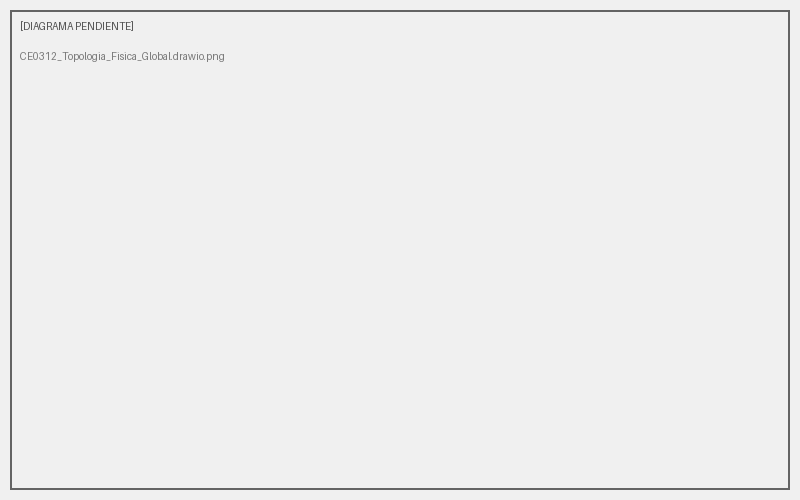
\includegraphics[width=0.95\textwidth]{CE0312_Topologia_Fisica_Global.drawio.png}
  \caption{Topología física global propuesta para Franco's SAC}
  \label{fig:topologia_fisica_global}
\end{figure}

La Figura \ref{fig:topologia_fisica_global} muestra la distribución física de los locales, enlaces de comunicación y la relación entre la sede central, sedes remotas y los servicios cloud. En esta vista se ve cómo se organiza la infraestructura antes de detallar la topología física por sede y segmentación lógica de la red.

\section{Arquitectura híbrida global}

La arquitectura híbrida global permite visualizar de forma integrada la distribución de los tres locales de Franco's SAC, la sede central, las sedes remotas, los hipervisores ESXi, los servicios internos, la zona DMZ, los microservicios, las bases de datos, los mecanismos de respaldo y la conexión con servicios cloud en AWS. Esta vista complementa la topología física global, ya que muestra con mayor detalle la relación entre infraestructura local, conectividad VPN, seguridad perimetral y servicios desplegados.

\begin{landscape}
\thispagestyle{fancy}

\begin{figure}[p]
  \centering
  \includegraphics[width=0.98\linewidth,height=0.82\textheight,keepaspectratio]{CE0312_Arquitectura_Hibrida_Global.png}
  \caption{Arquitectura híbrida global propuesta para Franco's SAC}
  \label{fig:arquitectura_hibrida_global}
\end{figure}

\end{landscape}

La Figura \ref{fig:arquitectura_hibrida_global} resume la arquitectura completa del diseño, mostrando la interacción entre las sedes, AWS, los enlaces VPN, la DMZ, los servicios internos, los microservicios y las bases de datos. Esta vista sirve como referencia general antes de detallar la topología física de cada sede.

\section{Topología física por sede}

La topología física por sede permite observar cómo se distribuyen los componentes tecnológicos en cada local de Franco's SAC. A nivel de diseño, no todos los locales cumplen el mismo rol: el Local 2 concentra la infraestructura principal, mientras que el Local 1 y el Local 3 operan como sedes remotas livianas conectadas hacia la sede central.

Esta separación permite organizar la infraestructura de acuerdo con la criticidad de los servicios. Los componentes expuestos, los servicios corporativos, los microservicios, las bases de datos y el monitoreo se concentran en la sede central; en cambio, las sedes remotas mantienen únicamente los elementos necesarios para operar localmente y comunicarse de forma segura con el hub principal.

\subsection{Topología física del Local 1}

El Local 1 representa la primera planta de producción de Franco's SAC. Su diseño físico corresponde a una sede remota liviana, compuesta por un hipervisor ESXi, un firewall local basado en pfSense, un controlador de dominio de solo lectura para autenticación local y servicios mínimos de archivos y monitoreo. Esta sede no aloja el ERP completo, sino que accede a los servicios principales mediante la VPN hacia el Local 2.

\begin{figure}[H]
  \centering
  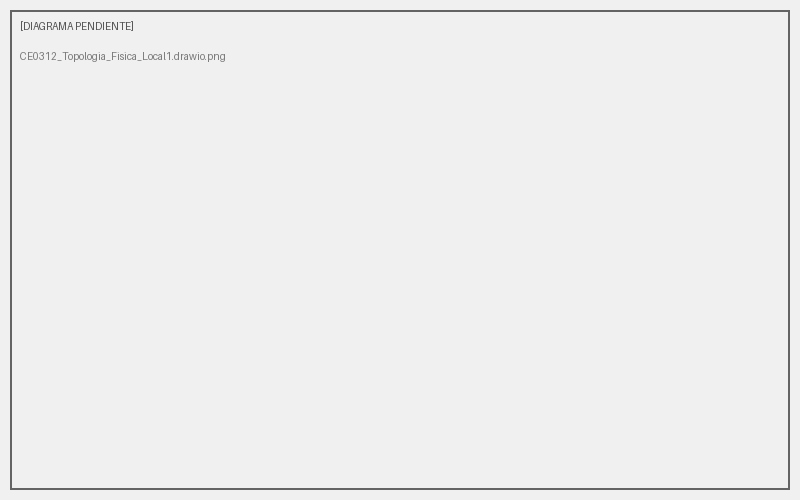
\includegraphics[width=0.92\textwidth]{CE0312_Topologia_Fisica_Local1.drawio.png}
  \caption{Topología física del Local 1 -- Planta de Producción 1}
  \label{fig:topologia_fisica_local_1}
\end{figure}

\subsection{Topología física del Local 2}

El Local 2 se define como la sede central de la infraestructura. En este punto se concentran los hipervisores principales, el firewall de borde, la zona DMZ, el WAF, el API Gateway, los servicios de autenticación, monitoreo, microservicios, bases de datos y respaldo crítico. Esta sede también funciona como punto central de interconexión para las VPN hacia el Local 1, Local 3 y AWS.

\begin{figure}[H]
  \centering
  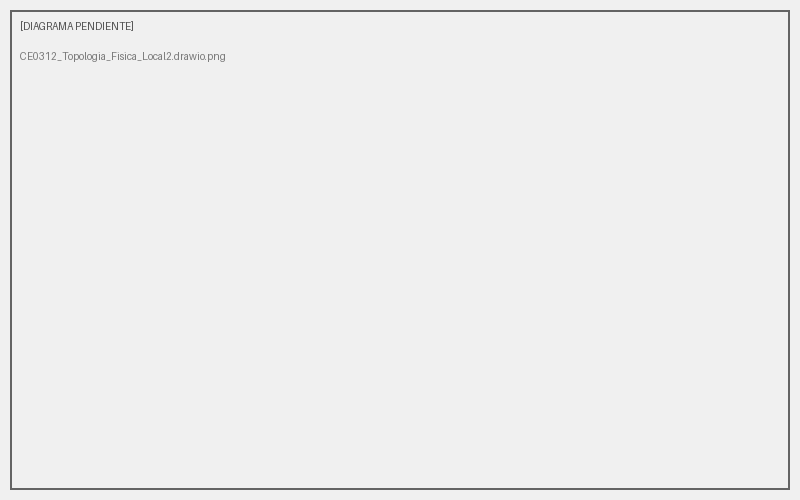
\includegraphics[width=0.92\textwidth]{CE0312_Topologia_Fisica_Local2.drawio.png}
  \caption{Topología física del Local 2 -- Sede Central}
  \label{fig:topologia_fisica_local_2}
\end{figure}

\subsection{Topología física del Local 3}

El Local 3 representa la segunda planta de producción. Su diseño físico mantiene la misma lógica aplicada al Local 1, debido a que también funciona como sede remota liviana. Por ello, cuenta con un hipervisor ESXi, pfSense local, autenticación mediante RODC y servicios mínimos para operación local. La diferencia principal se encuentra en el direccionamiento, los túneles VPN y los usuarios asociados a esta sede.

\begin{figure}[H]
  \centering
  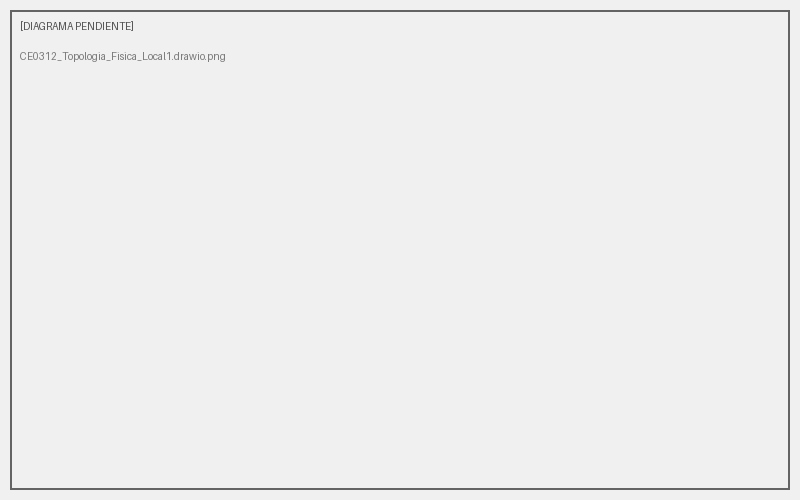
\includegraphics[width=0.92\textwidth]{CE0312_Topologia_Fisica_Local1.drawio.png}
  \caption{Topología física del Local 3 -- Segunda Planta de Producción}
  \label{fig:topologia_fisica_local_3}
\end{figure}


En conjunto, la distribución física por sede permite reducir la complejidad en los locales de producción y concentrar los servicios críticos en la sede central. Esta decisión facilita la administración de la infraestructura, mejora el control del tráfico y permite que el crecimiento futuro de Franco's SAC se apoye en una arquitectura ordenada y escalable.

\section{Arquitectura de vSwitches y port groups}

La arquitectura de vSwitches separa en cada hipervisor el tráfico WAN, el trunk 802.1Q y los port groups internos por VLAN. El criterio central es que pfSense recibe todas las VLANs internas vía trunk (VLAN ID 4095) y crea subinterfaces para actuar como gateway y firewall inter-VLAN en cada sede. Los hipervisores H1--H3 sirven la sede central (Local 2) con DMZ, servicios y datos; H4 y H5 replican la misma lógica para Local 1 y Local 3 respectivamente.

\begin{notabox}{Detalle completo}
La tabla con todos los vSwitches, port groups, VLAN IDs y propósitos de H1--H5 figura en el \textbf{Anexo~A} (pág.~\pageref{anex:vswitches}).
\end{notabox}
\section{Inventario de máquinas virtuales}

La sede central (Local 2) concentra el núcleo operativo: pfSense-BORDE, servicios de identidad (AD/DNS/NTP), WAF, microservicios ERP, bases de datos PostgreSQL, monitoreo Wazuh y respaldo. Las sedes remotas (Local 1 y Local 3) operan con una plantilla liviana: pfSense local, RODC y File Server. En total, el diseño considera 18 máquinas virtuales distribuidas en 5 hipervisores ESXi.

\begin{notabox}{Detalle completo}
El inventario con hostnames, IPs, recursos (vCPU/RAM/disco) y VLAN asignada figura en el \textbf{Anexo~B} (pág.~\pageref{anex:vms}).
\end{notabox}
\section{Topología lógica por sede}

La topología lógica define cómo se organiza internamente la red de Franco's SAC a través de VLANs, subredes, zonas funcionales y servicios asociados. A diferencia de la topología física, que muestra equipos y conexiones, la topología lógica permite comprender cómo se separa el tráfico, qué servicios se ubican en cada zona y cómo se controla la comunicación entre áreas.

En el diseño propuesto, el Local 2 concentra la mayor cantidad de segmentos lógicos debido a que funciona como sede central. En esta sede se ubican la DMZ, los servicios internos, las bases de datos, el monitoreo y la administración de la infraestructura. Por otro lado, el Local 1 y el Local 3 mantienen una estructura lógica más reducida, orientada a operación local, autenticación, gestión y acceso seguro hacia los servicios principales ubicados en la sede central.

\renewcommand{\arraystretch}{1.3}
\footnotesize
\hyphenpenalty=10000
\exhyphenpenalty=10000

\begin{xltabular}{\textwidth}{@{}|L{2.4cm}|L{3.1cm}|X|X|@{}}
\caption{Distribución lógica de servicios por sede}
\label{tab:topologia_logica_sedes} \\

\arrayrulecolor{upeu_dark}
\rowcolor{upeu_dark}
\parbox[c][1.1cm][c]{\linewidth}{\centering\color{white}\bfseries\small Sede} &
\parbox[c][1.1cm][c]{\linewidth}{\centering\color{white}\bfseries\small Rol lógico} &
\parbox[c][1.1cm][c]{\linewidth}{\centering\color{white}\bfseries\small Segmentos principales} &
\parbox[c][1.1cm][c]{\linewidth}{\centering\color{white}\bfseries\small Función dentro de la red} \\ \hline
\endfirsthead

\arrayrulecolor{upeu_dark}
\rowcolor{upeu_dark}
\parbox[c][1.1cm][c]{\linewidth}{\centering\color{white}\bfseries\small Sede} &
\parbox[c][1.1cm][c]{\linewidth}{\centering\color{white}\bfseries\small Rol lógico} &
\parbox[c][1.1cm][c]{\linewidth}{\centering\color{white}\bfseries\small Segmentos principales} &
\parbox[c][1.1cm][c]{\linewidth}{\centering\color{white}\bfseries\small Función dentro de la red} \\ \hline
\endhead

\hline
\endfoot

{\small Local 1} &
{\small Sede remota liviana} &
{\small VLAN 10 Administración, VLAN 20 Usuarios, VLAN 60 Gestión y VLAN 99 Management ESXi.} &
{\small Permite la operación básica de la primera planta de producción. Mantiene autenticación local mediante RODC, servicios mínimos de archivos, gestión del hipervisor y acceso seguro al ERP mediante VPN hacia la sede central.} \\ \hline

{\small Local 2} &
{\small Sede central y hub lógico} &
{\small VLAN 10 Administración, VLAN 20 Usuarios, VLAN 30 DMZ, VLAN 40 Servicios, VLAN 50 Datos, VLAN 60 Gestión y VLAN 99 Management ESXi.} &
{\small Aloja los servicios principales de la arquitectura: firewall de borde, WAF, API Gateway, Active Directory, monitoreo, microservicios, bases de datos, respaldo crítico y administración centralizada de la infraestructura.} \\ \hline

{\small Local 3} &
{\small Sede remota liviana} &
{\small VLAN 10 Administración, VLAN 20 Usuarios, VLAN 60 Gestión y VLAN 99 Management ESXi.} &
{\small Replica la lógica del Local 1 para la segunda planta de producción. Proporciona conectividad local, autenticación mediante RODC, gestión básica y acceso a los servicios corporativos alojados en la sede central.} \\ \hline

\end{xltabular}

\normalsize

La organización lógica por sede responde al principio de separación funcional. Las sedes remotas conservan únicamente los segmentos necesarios para operar de forma controlada, mientras que la sede central mantiene las zonas de mayor criticidad. Esta decisión evita exponer servicios sensibles en los locales de producción y permite administrar la seguridad desde un punto central.

\renewcommand{\arraystretch}{1.3}
\footnotesize
\hyphenpenalty=10000
\exhyphenpenalty=10000

\begin{xltabular}{\textwidth}{@{}|L{2.5cm}|C{1.5cm}|L{3cm}|X|@{}}
\caption{Resumen de VLANs y subredes por sede}
\label{tab:vlans_subredes_sede} \\

\arrayrulecolor{upeu_dark}
\rowcolor{upeu_dark}
\parbox[c][1.1cm][c]{\linewidth}{\centering\color{white}\bfseries\small Sede} &
\parbox[c][1.1cm][c]{\linewidth}{\centering\color{white}\bfseries\small VLAN} &
\parbox[c][1.1cm][c]{\linewidth}{\centering\color{white}\bfseries\small Nombre lógico} &
\parbox[c][1.1cm][c]{\linewidth}{\centering\color{white}\bfseries\small Subred asignada} \\ \hline
\endfirsthead

\arrayrulecolor{upeu_dark}
\rowcolor{upeu_dark}
\parbox[c][1.1cm][c]{\linewidth}{\centering\color{white}\bfseries\small Sede} &
\parbox[c][1.1cm][c]{\linewidth}{\centering\color{white}\bfseries\small VLAN} &
\parbox[c][1.1cm][c]{\linewidth}{\centering\color{white}\bfseries\small Nombre lógico} &
\parbox[c][1.1cm][c]{\linewidth}{\centering\color{white}\bfseries\small Subred asignada} \\ \hline
\endhead

\hline
\endfoot

{\small Local 2 -- Sede Central} & {\small 10} & {\small Administración} & {\small 10.10.10.0/24} \\ \hline
{\small Local 2 -- Sede Central} & {\small 20} & {\small Usuarios} & {\small 10.10.20.0/24} \\ \hline
{\small Local 2 -- Sede Central} & {\small 30} & {\small DMZ} & {\small 10.10.30.0/28} \\ \hline
{\small Local 2 -- Sede Central} & {\small 40} & {\small Servicios} & {\small 10.10.40.0/24} \\ \hline
{\small Local 2 -- Sede Central} & {\small 50} & {\small Datos} & {\small 10.10.50.0/28} \\ \hline
{\small Local 2 -- Sede Central} & {\small 60} & {\small Gestión} & {\small 10.10.60.0/28} \\ \hline
{\small Local 2 -- Sede Central} & {\small 99} & {\small Management ESXi} & {\small 10.10.99.0/28} \\ \hline

{\small Local 1 -- Planta Producción 1} & {\small 10} & {\small Administración} & {\small 10.20.10.0/24} \\ \hline
{\small Local 1 -- Planta Producción 1} & {\small 20} & {\small Usuarios} & {\small 10.20.20.0/24} \\ \hline
{\small Local 1 -- Planta Producción 1} & {\small 40} & {\small Servicios / FileServer} & {\small 10.20.40.0/24} \\ \hline
{\small Local 1 -- Planta Producción 1} & {\small 60} & {\small Gestión} & {\small 10.20.60.0/28} \\ \hline
{\small Local 1 -- Planta Producción 1} & {\small 99} & {\small Management ESXi} & {\small 10.20.99.0/28} \\ \hline

{\small Local 3 -- Segunda Planta} & {\small 10} & {\small Administración} & {\small 10.30.10.0/24} \\ \hline
{\small Local 3 -- Segunda Planta} & {\small 20} & {\small Usuarios} & {\small 10.30.20.0/24} \\ \hline
{\small Local 3 -- Segunda Planta} & {\small 40} & {\small Servicios / FileServer} & {\small 10.30.40.0/24} \\ \hline
{\small Local 3 -- Segunda Planta} & {\small 60} & {\small Gestión} & {\small 10.30.60.0/28} \\ \hline
{\small Local 3 -- Segunda Planta} & {\small 99} & {\small Management ESXi} & {\small 10.30.99.0/28} \\ \hline

\end{xltabular}

\normalsize

El esquema lógico de VLANs permite identificar rápidamente la sede y la función de cada segmento. En la convención utilizada, el segundo octeto diferencia la sede: \textbf{10.10.x.x} para Local 2, \textbf{10.20.x.x} para Local 1 y \textbf{10.30.x.x} para Local 3. A su vez, el tercer octeto representa la VLAN o zona funcional correspondiente.

\section{Conectividad interlocal mediante VPN}

La conectividad entre las sedes de Franco's SAC se plantea mediante una arquitectura VPN \textit{hub-and-spoke}, donde el Local 2 cumple el rol de sede central y punto principal de interconexión. Esta decisión permite centralizar el control del tráfico entre sedes, reducir la complejidad de enlaces directos y mantener una administración más ordenada de las rutas, políticas de seguridad y accesos hacia los servicios corporativos.

En este modelo, el Local 1 y el Local 3 no establecen comunicación directa entre sí; ambos se conectan hacia el Local 2, que actúa como concentrador de la red. De esta manera, todo acceso hacia el ERP, servicios internos, bases de datos, monitoreo y recursos cloud pasa por la sede central, permitiendo aplicar reglas de seguridad y trazabilidad desde un punto común.

La arquitectura también contempla un túnel adicional entre el Local 2 y AWS, con el objetivo de integrar servicios cloud complementarios como almacenamiento de respaldos, distribución de aplicaciones, repositorio de imágenes Docker y servicios de publicación externa. Esta conexión mantiene el enfoque híbrido del diseño, integrando infraestructura local con recursos en la nube bajo comunicación cifrada.

\begin{table}[H]
  \centering
  \renewcommand{\arraystretch}{1.3}
  \footnotesize
  \hyphenpenalty=10000
  \exhyphenpenalty=10000

  \begin{tabularx}{\textwidth}{@{}|L{2.2cm}|L{2.7cm}|L{2.8cm}|L{2.8cm}|X|@{}}

    \arrayrulecolor{upeu_dark}
    \rowcolor{upeu_dark}
    \parbox[c][1.1cm][c]{\linewidth}{\centering\color{white}\bfseries\small Túnel} &
    \parbox[c][1.1cm][c]{\linewidth}{\centering\color{white}\bfseries\small Subred} &
    \parbox[c][1.1cm][c]{\linewidth}{\centering\color{white}\bfseries\small IP Local 2} &
    \parbox[c][1.1cm][c]{\linewidth}{\centering\color{white}\bfseries\small IP remota} &
    \parbox[c][1.1cm][c]{\linewidth}{\centering\color{white}\bfseries\small Subredes enrutadas} \\ \hline

    {\small L1 -- L2} &
    {\small 172.16.10.0/30} &
    {\small 172.16.10.1} &
    {\small 172.16.10.2} &
    {\small 10.20.0.0/16 \(\leftrightarrow\) 10.10.0.0/16} \\ \hline

    {\small L2 -- L3} &
    {\small 172.16.20.0/30} &
    {\small 172.16.20.2} &
    {\small 172.16.20.1} &
    {\small 10.10.0.0/16 \(\leftrightarrow\) 10.30.0.0/16} \\ \hline

    {\small L2 -- AWS} &
    {\small 172.16.30.0/30} &
    {\small 172.16.30.2} &
    {\small 172.16.30.1} &
    {\small 10.10.0.0/16 \(\leftrightarrow\) 10.40.0.0/16} \\ \hline

  \end{tabularx}

  \caption{Túneles VPN considerados en la arquitectura interlocal}
  \label{tab:tuneles_vpn_interlocal}
\end{table}

Los túneles VPN se diseñan bajo un esquema de comunicación cifrada, priorizando confidencialidad, integridad y disponibilidad del tráfico entre sedes. En este contexto, el uso de IPSec con IKEv2 permite establecer enlaces seguros entre los firewalls pfSense de cada local y el gateway correspondiente en AWS.

\begin{table}[H]
  \centering
  \renewcommand{\arraystretch}{1.3}
  \footnotesize
  \hyphenpenalty=10000
  \exhyphenpenalty=10000

  \begin{tabularx}{0.95\textwidth}{@{}|L{3cm}|L{3.5cm}|X|@{}}

    \arrayrulecolor{upeu_dark}
    \rowcolor{upeu_dark}
    \parbox[c][1.1cm][c]{\linewidth}{\centering\color{white}\bfseries\small Parámetro} &
    \parbox[c][1.1cm][c]{\linewidth}{\centering\color{white}\bfseries\small Valor definido} &
    \parbox[c][1.1cm][c]{\linewidth}{\centering\color{white}\bfseries\small Justificación técnica} \\ \hline

    {\small Protocolo VPN} &
    {\small IPSec IKEv2} &
    {\small Permite establecer túneles seguros entre sedes con mejor estabilidad y administración que versiones anteriores.} \\ \hline

    {\small Cifrado} &
    {\small AES-256-GCM} &
    {\small Proporciona cifrado robusto para proteger la confidencialidad del tráfico entre locales y AWS.} \\ \hline

    {\small Integridad} &
    {\small SHA-256} &
    {\small Garantiza la validación de integridad de los datos transmitidos por el túnel.} \\ \hline

    {\small Grupo Diffie-Hellman} &
    {\small Group 14} &
    {\small Permite establecer intercambio seguro de claves con un nivel adecuado para el escenario propuesto.} \\ \hline

    {\small Detección de caída} &
    {\small DPD habilitado} &
    {\small Permite identificar la caída de un extremo VPN y facilitar la reconexión del túnel.} \\ \hline

    {\small NAT Traversal} &
    {\small Habilitado} &
    {\small Facilita el funcionamiento de los túneles en el entorno de laboratorio, donde los enlaces pueden estar detrás de NAT.} \\ \hline

  \end{tabularx}

  \caption{Parámetros técnicos definidos para los túneles IPSec}
  \label{tab:parametros_ipsec}
\end{table}

Con esta configuración, la conectividad interlocal mantiene una estructura segura y controlada. El Local 2 concentra la administración del tráfico entre sedes, mientras que los locales remotos acceden a los servicios corporativos sin exponer directamente las redes internas. Este enfoque también facilita la integración con AWS y deja preparada la infraestructura para políticas posteriores de segmentación, monitoreo y alta disponibilidad.

\section{Esquema de direccionamiento IP}

El esquema usa convención jerárquica por octeto: Local 2 en \textbf{10.10.x.x}, Local 1 en \textbf{10.20.x.x}, Local 3 en \textbf{10.30.x.x} y VPC AWS en \textbf{10.40.x.x}. Los túneles VPN punto a punto usan \textbf{/30} en el rango \textbf{172.16.x.x}. Las VLANs de gestión y monitoreo emplean \textbf{/28} para limitar la superficie de exposición; las zonas operativas de usuarios y servicios usan \textbf{/24}.

\begin{notabox}{Detalle completo}
Las tablas con subredes, máscaras, gateways, rangos DHCP y direcciones estáticas por sede figuran en el \textbf{Anexo~C} (pág.~\pageref{anex:ip}).
\end{notabox}
\section{Flujos de tráfico por zona}

La segmentación no solo separa redes: define qué comunicaciones se permiten. El principio rector es \textit{deny-all con excepciones explícitas}: los usuarios acceden al ERP vía API Gateway pero nunca directamente a las BD; la DMZ recibe tráfico externo controlado pero no tiene acceso abierto hacia zonas internas; las sedes remotas se comunican con la sede central únicamente por VPN IPSec.

\begin{notabox}{Detalle completo}
Las matrices de flujos permitidos/bloqueados por par de zonas (VLAN origen \textrightarrow{} VLAN destino) figuran en el \textbf{Anexo~D} (pág.~\pageref{anex:flujos}).
\end{notabox}
\section{Alineación con estándares internacionales}

El diseño de la topología lógica y física no se plantea únicamente como una distribución de equipos, redes y servicios, sino como una propuesta alineada con criterios técnicos reconocidos. Por ello, se consideran estándares relacionados con segmentación de red, cableado estructurado, conectividad Ethernet, seguridad de comunicaciones y separación de zonas.

Esta alineación permite sustentar que la infraestructura propuesta mantiene una base técnica válida para un escenario empresarial. Además, facilita que el diseño pueda ser evaluado no solo por su funcionalidad, sino también por su coherencia con buenas prácticas de conectividad, seguridad y administración de infraestructura.

\renewcommand{\arraystretch}{1.3}
\footnotesize
\hyphenpenalty=10000
\exhyphenpenalty=10000

\begin{xltabular}{\textwidth}{@{}|L{3cm}|X|X|@{}}
\caption{Alineación del diseño con estándares internacionales}
\label{tab:alineacion_estandares_internacionales} \\

\arrayrulecolor{upeu_dark}
\rowcolor{upeu_dark}
\parbox[c][1.1cm][c]{\linewidth}{\centering\color{white}\bfseries\small Estándar} &
\parbox[c][1.1cm][c]{\linewidth}{\centering\color{white}\bfseries\small Aplicación en el diseño} &
\parbox[c][1.1cm][c]{\linewidth}{\centering\color{white}\bfseries\small Justificación técnica} \\ \hline
\endfirsthead

\arrayrulecolor{upeu_dark}
\rowcolor{upeu_dark}
\parbox[c][1.1cm][c]{\linewidth}{\centering\color{white}\bfseries\small Estándar} &
\parbox[c][1.1cm][c]{\linewidth}{\centering\color{white}\bfseries\small Aplicación en el diseño} &
\parbox[c][1.1cm][c]{\linewidth}{\centering\color{white}\bfseries\small Justificación técnica} \\ \hline
\endhead

\hline
\endfoot

{\small IEEE 802.1Q\newline \cite{ieee8021q}} &
{\small Se aplica en la segmentación de red mediante VLANs y en el uso de enlaces troncales entre switches, hipervisores ESXi y pfSense.} &
{\small Permite separar lógicamente el tráfico por zonas funcionales como administración, usuarios, DMZ, servicios, datos, gestión y management. Esta separación reduce la exposición entre segmentos y permite aplicar reglas de seguridad más específicas.} \\ \hline

{\small IEEE 802.3} &
{\small Se considera en los enlaces Ethernet físicos utilizados por hipervisores, switches, routers, firewalls y dispositivos finales del entorno de laboratorio.} &
{\small Proporciona la base para la conectividad cableada de la infraestructura, permitiendo representar enlaces LAN y WAN de forma coherente dentro del diseño físico propuesto.} \\ \hline

{\small TIA/EIA-568\newline \cite{tiaeia568c2}} &
{\small Se toma como referencia para la organización del cableado estructurado y la distribución física de puntos de red, enlaces y equipos de comunicación.} &
{\small Favorece una infraestructura ordenada, documentada y preparada para crecimiento, considerando buenas prácticas de conexión entre equipos de red, servidores, hipervisores y estaciones de trabajo.} \\ \hline

{\small ISO/IEC 11801} &
{\small Se aplica como referencia para el cableado genérico en instalaciones de cliente y para la organización funcional de los canales de comunicación.} &
{\small Refuerza la necesidad de mantener una red organizada por funciones, diferenciando tráfico de usuarios, gestión, servicios críticos, datos y administración de infraestructura.} \\ \hline

{\small NIST SP 800-53} &
{\small Se relaciona con la segmentación de zonas, protección perimetral, control de tráfico, separación de sistemas y confidencialidad de las comunicaciones.} &
{\small Sustenta el uso de DMZ, firewall, VPN IPSec, separación entre servicios y datos, monitoreo, control de acceso y aplicación del principio de mínimo privilegio en los flujos de red.} \\ \hline

\end{xltabular}

\normalsize

La aplicación de estos estándares fortalece la validez técnica del diseño propuesto. En particular, la segmentación mediante VLANs, el uso de enlaces troncales, la separación entre zonas críticas, la protección de comunicaciones mediante VPN y la organización física de la red permiten que la arquitectura sea más segura, administrable y escalable.


% ── CE0313 ──────────────────────────────────────────────────
\chapter{CE0313 - Segmentacion de Red (VLAN, DMZ, Subnetting)}

\section{Criterios de segmentación de red}

La segmentación de red propuesta para Franco's SAC se plantea como una decisión técnica orientada a ordenar, proteger y controlar la comunicación entre las distintas áreas, sedes y servicios de la organización. No se trata únicamente de dividir la red en varias VLANs, sino de establecer zonas funcionales con propósitos definidos, rangos IP diferenciados y reglas de comunicación controladas.

A partir del diseño lógico y físico definido previamente, la segmentación se estructura considerando tres sedes: Local 2 como sede central, Local 1 como primera planta de producción y Local 3 como segunda planta de producción. Esta distribución permite que los servicios críticos, como la DMZ, microservicios, bases de datos, monitoreo y respaldo, se mantengan concentrados en la sede central; mientras que las sedes remotas conservan una estructura liviana para usuarios, autenticación local, gestión y administración del hipervisor.

El criterio principal del diseño es aplicar separación funcional. Por ello, los usuarios no comparten red con las bases de datos, la DMZ no accede directamente a la capa de datos, la gestión técnica se mantiene aislada de las estaciones de trabajo y la administración de ESXi se ubica en una red independiente. Esta organización reduce dominios de broadcast, mejora el control del tráfico y limita el impacto ante posibles incidentes de seguridad.

\renewcommand{\arraystretch}{1.3}
\footnotesize
\hyphenpenalty=10000
\exhyphenpenalty=10000

\begin{xltabular}{\textwidth}{@{}|N{1.5cm}|L{3.8cm}|X|X|@{}}
\caption{Criterios aplicados a la segmentación de red}
\label{tab:criterios_segmentacion_red} \\

\arrayrulecolor{upeu_dark}
\rowcolor{upeu_dark}
\parbox[c][1.1cm][c]{\linewidth}{\centering\color{white}\bfseries\small Código} &
\parbox[c][1.1cm][c]{\linewidth}{\centering\color{white}\bfseries\small Criterio} &
\parbox[c][1.1cm][c]{\linewidth}{\centering\color{white}\bfseries\small Aplicación en el diseño} &
\parbox[c][1.1cm][c]{\linewidth}{\centering\color{white}\bfseries\small Justificación técnica} \\ \hline
\endfirsthead

\arrayrulecolor{upeu_dark}
\rowcolor{upeu_dark}
\parbox[c][1.1cm][c]{\linewidth}{\centering\color{white}\bfseries\small Código} &
\parbox[c][1.1cm][c]{\linewidth}{\centering\color{white}\bfseries\small Criterio} &
\parbox[c][1.1cm][c]{\linewidth}{\centering\color{white}\bfseries\small Aplicación en el diseño} &
\parbox[c][1.1cm][c]{\linewidth}{\centering\color{white}\bfseries\small Justificación técnica} \\ \hline
\endhead

\hline
\endfoot

{\small CS-01} &
{\small Separación por función} &
{\small Se definen VLANs independientes para administración, usuarios, DMZ, servicios, datos, gestión y administración ESXi.} &
{\small Permite evitar que todo el tráfico de la organización comparta el mismo dominio de red, reduciendo desorden operativo y exposición innecesaria.} \\ \hline

{\small CS-02} &
{\small Sede central como núcleo de servicios} &
{\small El Local 2 concentra las VLANs críticas: DMZ, servicios, datos, monitoreo, administración y usuarios corporativos.} &
{\small Centralizar los servicios principales facilita la administración, el monitoreo, la aplicación de reglas de seguridad y la continuidad operativa.} \\ \hline

{\small CS-03} &
{\small Sedes remotas livianas} &
{\small El Local 1 y el Local 3 mantienen solo VLANs de administración, usuarios, gestión y management ESXi.} &
{\small Las plantas de producción no requieren alojar bases de datos, DMZ ni microservicios; acceden a los servicios centrales mediante VPN.} \\ \hline

{\small CS-04} &
{\small DMZ exclusiva para exposición controlada} &
{\small La VLAN 30 se ubica únicamente en el Local 2 y aloja componentes como WAF y API Gateway.} &
{\small La DMZ funciona como zona intermedia entre redes externas y servicios internos, evitando la exposición directa de microservicios y bases de datos.} \\ \hline

{\small CS-05} &
{\small Subredes dimensionadas según criticidad} &
{\small Se utilizan redes /24 para segmentos con crecimiento operativo y redes /28 para zonas críticas o reducidas.} &
{\small Las VLANs de usuarios, administración y servicios requieren mayor capacidad; en cambio, DMZ, datos, gestión y management se limitan para reducir superficie de ataque.} \\ \hline

{\small CS-06} &
{\small Routing inter-VLAN controlado} &
{\small pfSense actúa como gateway de las VLANs mediante subinterfaces asociadas a cada segmento.} &
{\small La comunicación entre VLANs no debe ser libre; debe pasar por reglas de firewall que permitan, restrinjan o bloqueen el tráfico según la función de cada zona.} \\ \hline

{\small CS-07} &
{\small Transporte de VLANs mediante trunk} &
{\small Se emplea IEEE 802.1Q para transportar múltiples VLANs entre ESXi, pfSense y el switch de distribución.} &
{\small El uso de trunk permite consolidar múltiples redes lógicas sobre enlaces físicos controlados, manteniendo separación mediante etiquetado VLAN.} \\ \hline

{\small CS-08} &
{\small Principio de mínimo privilegio} &
{\small Los usuarios no acceden directamente a bases de datos, la DMZ no consulta datos de forma directa y la gestión técnica se limita a personal autorizado.} &
{\small Cada comunicación permitida debe responder a una necesidad operativa concreta, reduciendo riesgos por accesos innecesarios entre zonas.} \\ \hline

\end{xltabular}

\normalsize

Estos criterios permiten que la segmentación de red sea coherente con la arquitectura general propuesta. La división por VLANs, el uso de DMZ, el direccionamiento jerárquico y el control mediante pfSense establecen una base ordenada para los siguientes bloques del CE0313, donde se detallan las VLANs por sede, los cálculos de subnetting, las subredes VPN, el routing inter-VLAN y la configuración trunk IEEE 802.1Q.

\section{Resumen general de VLANs por sede}

El esquema de segmentación propuesto para Franco's SAC se organiza en tres sedes con rangos IP diferenciados. La sede central, correspondiente al Local 2, concentra los segmentos de mayor criticidad, mientras que el Local 1 y el Local 3 mantienen una estructura más reducida orientada a operación productiva y acceso seguro hacia los servicios centrales.

En total, el diseño considera \textbf{17 VLANs}: siete VLANs en el Local 2, cinco VLANs en el Local 1 y cinco VLANs en el Local 3. La VLAN 40 (Servicios) se replica en los tres locales para alojar el servidor de archivos local en las sedes remotas, mientras que la sede central añade microservicios y NATS en la misma zona. Esta separación permite ordenar el tráfico de administración, usuarios, DMZ, servicios, datos, gestión técnica y administración de hipervisores.

\renewcommand{\arraystretch}{1.3}
\footnotesize
\hyphenpenalty=10000
\exhyphenpenalty=10000

\begin{xltabular}{\textwidth}{@{}|L{3.2cm}|L{3cm}|N{2cm}|X|@{}}
\caption{Resumen de segmentación por sede}
\label{tab:resumen_segmentacion_sede} \\

\arrayrulecolor{upeu_dark}
\rowcolor{upeu_dark}
\parbox[c][1.1cm][c]{\linewidth}{\centering\color{white}\bfseries\small Sede} &
\parbox[c][1.1cm][c]{\linewidth}{\centering\color{white}\bfseries\small Rango base} &
\parbox[c][1.1cm][c]{\linewidth}{\centering\color{white}\bfseries\small VLANs} &
\parbox[c][1.1cm][c]{\linewidth}{\centering\color{white}\bfseries\small Rol dentro de la segmentación} \\ \hline
\endfirsthead

\arrayrulecolor{upeu_dark}
\rowcolor{upeu_dark}
\parbox[c][1.1cm][c]{\linewidth}{\centering\color{white}\bfseries\small Sede} &
\parbox[c][1.1cm][c]{\linewidth}{\centering\color{white}\bfseries\small Rango base} &
\parbox[c][1.1cm][c]{\linewidth}{\centering\color{white}\bfseries\small VLANs} &
\parbox[c][1.1cm][c]{\linewidth}{\centering\color{white}\bfseries\small Rol dentro de la segmentación} \\ \hline
\endhead

\hline
\endfoot

{\small Local 2 -- Sede Central} &
{\small 10.10.0.0/16} &
{\small 7} &
{\small Actúa como núcleo de la infraestructura. Aloja administración, usuarios corporativos, DMZ, servicios internos, bases de datos, monitoreo y administración de hipervisores.} \\ \hline

{\small Local 1 -- Planta de Producción 1} &
{\small 10.20.0.0/16} &
{\small 5} &
{\small Opera como sede remota liviana. Mantiene segmentos para administración/RODC (VLAN10), usuarios (VLAN20), servicios/FileServer (VLAN40), gestión/Wazuh-agent (VLAN60) y Management ESXi (VLAN99). H4.} \\ \hline

{\small Local 3 -- Segunda Planta de Producción} &
{\small 10.30.0.0/16} &
{\small 5} &
{\small Replica la estructura del Local 1: VLAN10/VLAN20/VLAN40/VLAN60/VLAN99. Incluye RODC DC4, FileServer-L3 y agentes Wazuh. H5 se documenta con referencia logica de laboratorio.} \\ \hline

\end{xltabular}

\normalsize

La lógica de direccionamiento permite reconocer la sede desde el segundo octeto: \textbf{10.10.x.x} para el Local 2, \textbf{10.20.x.x} para el Local 1 y \textbf{10.30.x.x} para el Local 3. Esta convención facilita la administración de rutas, reglas de firewall, monitoreo y documentación técnica.

\begin{landscape}
\thispagestyle{fancy}

\renewcommand{\arraystretch}{1.3}
\footnotesize
\hyphenpenalty=10000
\exhyphenpenalty=10000

\begin{xltabular}{\linewidth}{@{}|N{1.5cm}|L{2.6cm}|L{3.5cm}|L{3.5cm}|L{3.5cm}|X|@{}}
\caption{Vista consolidada de VLANs por sede}
\label{tab:vista_consolidada_vlans_sede} \\

\arrayrulecolor{upeu_dark}
\rowcolor{upeu_dark}
\parbox[c][1.1cm][c]{\linewidth}{\centering\color{white}\bfseries\small VLAN} &
\parbox[c][1.1cm][c]{\linewidth}{\centering\color{white}\bfseries\small Nombre lógico} &
\parbox[c][1.1cm][c]{\linewidth}{\centering\color{white}\bfseries\small Local 2 -- Sede Central} &
\parbox[c][1.1cm][c]{\linewidth}{\centering\color{white}\bfseries\small Local 1 -- Producción} &
\parbox[c][1.1cm][c]{\linewidth}{\centering\color{white}\bfseries\small Local 3 -- Segunda planta} &
\parbox[c][1.1cm][c]{\linewidth}{\centering\color{white}\bfseries\small Propósito general} \\ \hline
\endfirsthead

\arrayrulecolor{upeu_dark}
\rowcolor{upeu_dark}
\parbox[c][1.1cm][c]{\linewidth}{\centering\color{white}\bfseries\small VLAN} &
\parbox[c][1.1cm][c]{\linewidth}{\centering\color{white}\bfseries\small Nombre lógico} &
\parbox[c][1.1cm][c]{\linewidth}{\centering\color{white}\bfseries\small Local 2 -- Sede Central} &
\parbox[c][1.1cm][c]{\linewidth}{\centering\color{white}\bfseries\small Local 1 -- Producción} &
\parbox[c][1.1cm][c]{\linewidth}{\centering\color{white}\bfseries\small Local 3 -- Segunda planta} &
\parbox[c][1.1cm][c]{\linewidth}{\centering\color{white}\bfseries\small Propósito general} \\ \hline
\endhead

\hline
\endfoot

{\small 10} &
{\small Administración} &
{\small 10.10.10.0/24} &
{\small 10.20.10.0/24} &
{\small 10.30.10.0/24} &
{\small Segmento destinado a servicios administrativos, autenticación, DNS, NTP y controladores de dominio o RODC según la sede.} \\ \hline

{\small 20} &
{\small Usuarios} &
{\small 10.10.20.0/24} &
{\small 10.20.20.0/24} &
{\small 10.30.20.0/24} &
{\small Segmento para estaciones de trabajo, usuarios internos, operarios y acceso al ERP mediante navegación o conexión segura.} \\ \hline

{\small 30} &
{\small DMZ} &
{\small 10.10.30.0/28} &
{\small --} &
{\small --} &
{\small Zona desmilitarizada exclusiva de la sede central, utilizada para alojar el WAF y el API Gateway como punto de exposición controlada.} \\ \hline

{\small 40} &
{\small Servicios} &
{\small 10.10.40.0/24} &
{\small 10.20.40.0/24} &
{\small 10.30.40.0/24} &
{\small L2: microservicios NestJS, NATS JetStream y FileServer central. L1/L3: solo FileServer local (VM-FileServer-L1/L3). VLAN 40 en los 3 locales para coherencia estructural.} \\ \hline

{\small 50} &
{\small Datos} &
{\small 10.10.50.0/28} &
{\small --} &
{\small --} &
{\small Segmento crítico para bases de datos PostgreSQL. Su acceso debe estar restringido únicamente a servicios autorizados.} \\ \hline

{\small 60} &
{\small Gestión} &
{\small 10.10.60.0/28} &
{\small 10.20.60.0/28} &
{\small 10.30.60.0/28} &
{\small Red destinada al monitoreo híbrido (Wazuh + CloudWatch), supervisión técnica, agentes Wazuh, ICMP, SNMP y administración controlada de servicios.} \\ \hline

{\small 99} &
{\small Management ESXi} &
{\small 10.10.99.0/28} &
{\small 10.20.99.0/28} &
{\small 10.30.99.0/28} &
{\small Segmento aislado para administración de hipervisores ESXi, interfaces VMkernel y gestión técnica de la plataforma virtual.} \\ \hline

\end{xltabular}

\normalsize
\end{landscape}

La vista consolidada evidencia que no todas las VLANs se replican en todas las sedes. Las VLANs 30, 40 y 50 se mantienen únicamente en el Local 2 porque allí se concentran la DMZ, los servicios del ERP y las bases de datos. En cambio, los locales 1 y 3 conservan solo los segmentos necesarios para operar como sedes remotas, reduciendo complejidad y superficie de exposición.

\section{Diseño detallado de VLANs por sede}

La segmentación de red por sede se basa en el esquema resumido presentado en la sección anterior. La sede central (Local~2) incorpora las 7 VLANs completas: Administración (10), Usuarios (20), DMZ (30), Servicios (40), Datos (50), Gestión (60) y Management ESXi (99). Las sedes remotas (Local~1 y Local~3) mantienen una segmentación reducida de 5 VLANs cada una, suprimiendo la DMZ y la VLAN de Datos que permanecen centralizadas en Local~2. El detalle completo de subredes, gateways y criterios de segmentación por VLAN y por sede se encuentra en el Anexo~I.

\section{Diseño de la DMZ}

La DMZ se define como una zona de red intermedia entre los accesos externos y los servicios internos de Franco's SAC. En el diseño propuesto, esta zona se implementa únicamente en la sede central, debido a que allí se concentran los servicios expuestos de forma controlada, como el WAF y el API Gateway.

A diferencia de las VLANs internas, la DMZ no debe considerarse una red de confianza completa. Su función es recibir tráfico autorizado, inspeccionarlo y canalizarlo hacia los servicios correspondientes sin exponer directamente la red de servicios ni la red de datos. Por ello, se ubica en una subred reducida \textbf{/28}, suficiente para los componentes previstos y coherente con el principio de mínima superficie de exposición.

\renewcommand{\arraystretch}{1.3}
\footnotesize
\hyphenpenalty=10000
\exhyphenpenalty=10000

\begin{xltabular}{\textwidth}{@{}|L{3cm}|L{3.2cm}|X|X|@{}}
\caption{Componentes definidos para la DMZ}
\label{tab:componentes_dmz} \\

\arrayrulecolor{upeu_dark}
\rowcolor{upeu_dark}
\parbox[c][1.1cm][c]{\linewidth}{\centering\color{white}\bfseries\small Componente} &
\parbox[c][1.1cm][c]{\linewidth}{\centering\color{white}\bfseries\small Dirección IP} &
\parbox[c][1.1cm][c]{\linewidth}{\centering\color{white}\bfseries\small Función principal} &
\parbox[c][1.1cm][c]{\linewidth}{\centering\color{white}\bfseries\small Criterio de seguridad} \\ \hline
\endfirsthead

\arrayrulecolor{upeu_dark}
\rowcolor{upeu_dark}
\parbox[c][1.1cm][c]{\linewidth}{\centering\color{white}\bfseries\small Componente} &
\parbox[c][1.1cm][c]{\linewidth}{\centering\color{white}\bfseries\small Dirección IP} &
\parbox[c][1.1cm][c]{\linewidth}{\centering\color{white}\bfseries\small Función principal} &
\parbox[c][1.1cm][c]{\linewidth}{\centering\color{white}\bfseries\small Criterio de seguridad} \\ \hline
\endhead

\hline
\endfoot

{\small Gateway DMZ} &
{\small 10.10.30.1} &
{\small Corresponde a la interfaz de pfSense-BORDE para la VLAN 30. Actúa como puerta de enlace y punto de control del tráfico que entra y sale de la DMZ.} &
{\small Todo tráfico hacia otras VLANs debe pasar por reglas explícitas de firewall, evitando comunicación libre con zonas internas.} \\ \hline

{\small VM-WAF} &
{\small 10.10.30.5} &
{\small Componente de protección web encargado de inspeccionar solicitudes HTTP/HTTPS antes de que lleguen al API Gateway.} &
{\small Reduce la exposición de la aplicación ante tráfico malicioso y permite aplicar filtrado a nivel de capa de aplicación.} \\ \hline

{\small VM-API-GATEWAY} &
{\small 10.10.30.10} &
{\small Punto de entrada lógico hacia el ERP. Recibe las solicitudes validadas y las canaliza hacia la capa de servicios autorizada.} &
{\small Evita que los usuarios o accesos externos lleguen directamente a microservicios o bases de datos.} \\ \hline

{\small VM-BACKUP-API-GW} &
{\small 10.10.30.11} &
{\small Componente de contingencia del API Gateway, reservado para escenarios de respaldo o recuperación.} &
{\small Se mantiene dentro del rango válido de la subred 10.10.30.0/28, evitando asignaciones fuera del segmento definido.} \\ \hline

\end{xltabular}

\normalsize

La subred \textbf{10.10.30.0/28} permite utilizar direcciones desde \textbf{10.10.30.1} hasta \textbf{10.10.30.14}, considerando el gateway y los hosts disponibles. Por esta razón, el componente de respaldo del API Gateway se asigna como \textbf{10.10.30.11}, manteniéndose dentro del rango válido de la DMZ.

\renewcommand{\arraystretch}{1.3}
\footnotesize
\hyphenpenalty=10000
\exhyphenpenalty=10000

\begin{xltabular}{\textwidth}{@{}|L{3.3cm}|L{3.3cm}|L{2.7cm}|X|@{}}
\caption{Reglas base consideradas para la DMZ}
\label{tab:reglas_base_dmz} \\

\arrayrulecolor{upeu_dark}
\rowcolor{upeu_dark}
\parbox[c][1.1cm][c]{\linewidth}{\centering\color{white}\bfseries\small Origen} &
\parbox[c][1.1cm][c]{\linewidth}{\centering\color{white}\bfseries\small Destino} &
\parbox[c][1.1cm][c]{\linewidth}{\centering\color{white}\bfseries\small Estado} &
\parbox[c][1.1cm][c]{\linewidth}{\centering\color{white}\bfseries\small Justificación} \\ \hline
\endfirsthead

\arrayrulecolor{upeu_dark}
\rowcolor{upeu_dark}
\parbox[c][1.1cm][c]{\linewidth}{\centering\color{white}\bfseries\small Origen} &
\parbox[c][1.1cm][c]{\linewidth}{\centering\color{white}\bfseries\small Destino} &
\parbox[c][1.1cm][c]{\linewidth}{\centering\color{white}\bfseries\small Estado} &
\parbox[c][1.1cm][c]{\linewidth}{\centering\color{white}\bfseries\small Justificación} \\ \hline
\endhead

\hline
\endfoot

{\small Internet o acceso externo autorizado} &
{\small VM-WAF} &
{\small Permitido controlado} &
{\small El ingreso externo debe pasar primero por la capa de protección web, evitando exposición directa del API Gateway.} \\ \hline

{\small VM-WAF} &
{\small VM-API-GATEWAY} &
{\small Permitido} &
{\small El WAF reenvía únicamente tráfico inspeccionado hacia el punto de entrada del ERP.} \\ \hline

{\small VM-API-GATEWAY} &
{\small VLAN 40 -- Servicios} &
{\small Permitido restringido} &
{\small El API Gateway puede comunicarse con la capa de servicios solo mediante los puertos definidos para la operación del ERP.} \\ \hline

{\small VLAN 30 -- DMZ} &
{\small VLAN 50 -- Datos} &
{\small Denegado} &
{\small La DMZ no debe consultar bases de datos directamente. Toda operación debe pasar por la capa de servicios.} \\ \hline

{\small VLAN 20 -- Usuarios} &
{\small VLAN 30 -- DMZ} &
{\small Permitido} &
{\small Los usuarios acceden al ERP mediante el punto de entrada publicado, sin conectarse directamente a servicios internos.} \\ \hline

\end{xltabular}

\normalsize

Con esta configuración, la DMZ cumple una función de contención y exposición controlada. La red pública o de acceso externo no llega directamente a la capa de servicios ni a la capa de datos; primero atraviesa el WAF y luego el API Gateway. Este diseño reduce el impacto ante un posible incidente en la zona expuesta, ya que las bases de datos y los microservicios permanecen separados en VLANs internas.

\section{Cálculos de subnetting}

El diseño emplea tres tamaños: \textbf{/24} para zonas operativas con crecimiento (usuarios, servicios), \textbf{/28} para segmentos críticos o reducidos (gestión, monitoreo), y \textbf{/30} para enlaces punto a punto entre sedes y AWS. Esta combinación balancea capacidad, orden y mínima superficie de exposición.

\section{Subredes VPN hub-and-spoke}

Las sedes remotas y AWS no se conectan entre sí directamente; cada una establece su túnel hacia el Local 2 (hub). Se usan subredes \textbf{/30} en el rango \textbf{172.16.x.x} para cada enlace.

\begin{notabox}{Detalle completo}
Los cálculos detallados de subnetting y la tabla de subredes VPN figuran en el \textbf{Anexo~E} (pág.~\pageref{anex:subnetting}).
\end{notabox}
\section{Inter-VLAN routing con pfSense}

pfSense implementa \textit{Router-on-a-Stick}: recibe todas las VLANs etiquetadas sobre una sola interfaz trunk y crea subinterfaces (p.\,ej., \texttt{em2.10}, \texttt{em2.20}) que actúan como gateway y punto de control por segmento, con reglas de firewall independientes por VLAN.

\section{Configuración trunk IEEE 802.1Q}

El estándar IEEE 802.1Q etiqueta las tramas con el VLAN ID correspondiente, permitiendo que ESXi, pfSense y los switches reconozcan a qué red lógica pertenece cada paquete. El port group \texttt{PG-TRUNK} usa VLAN ID 4095 en ESXi para pasar todas las VLANs al pfSense sin filtrar.

\begin{notabox}{Detalle completo}
Las tablas de subinterfaces pfSense, comandos de configuración trunk y reglas base inter-VLAN figuran en el \textbf{Anexo~F} (pág.~\pageref{anex:routing}).
\end{notabox}
\section{Reglas base de segmentación entre VLANs}

La segmentación mediante VLANs solo es efectiva si se acompaña de reglas de comunicación claras. Por ello, el diseño de Franco's SAC no plantea una red donde todas las VLANs puedan comunicarse libremente, sino una arquitectura donde cada flujo debe responder a una necesidad operativa específica.

En este bloque se resumen las reglas base de segmentación. No se busca repetir toda la matriz de flujos definida previamente, sino establecer los criterios principales que deben aplicarse en pfSense para controlar la comunicación entre usuarios, DMZ, servicios, datos, gestión y administración de infraestructura.

\renewcommand{\arraystretch}{1.3}
\footnotesize
\hyphenpenalty=10000
\exhyphenpenalty=10000

\begin{xltabular}{\textwidth}{@{}|L{3cm}|L{3cm}|L{2.4cm}|X|@{}}
\caption{Reglas base de segmentación entre VLANs}
\label{tab:reglas_base_segmentacion_vlans} \\

\arrayrulecolor{upeu_dark}
\rowcolor{upeu_dark}
\parbox[c][1.1cm][c]{\linewidth}{\centering\color{white}\bfseries\small Origen} &
\parbox[c][1.1cm][c]{\linewidth}{\centering\color{white}\bfseries\small Destino} &
\parbox[c][1.1cm][c]{\linewidth}{\centering\color{white}\bfseries\small Estado} &
\parbox[c][1.1cm][c]{\linewidth}{\centering\color{white}\bfseries\small Criterio de control} \\ \hline
\endfirsthead

\arrayrulecolor{upeu_dark}
\rowcolor{upeu_dark}
\parbox[c][1.1cm][c]{\linewidth}{\centering\color{white}\bfseries\small Origen} &
\parbox[c][1.1cm][c]{\linewidth}{\centering\color{white}\bfseries\small Destino} &
\parbox[c][1.1cm][c]{\linewidth}{\centering\color{white}\bfseries\small Estado} &
\parbox[c][1.1cm][c]{\linewidth}{\centering\color{white}\bfseries\small Criterio de control} \\ \hline
\endhead

\hline
\endfoot

{\small VLAN 20 -- Usuarios} &
{\small VLAN 30 -- DMZ} &
{\small Permitido} &
{\small Los usuarios pueden acceder al ERP mediante el punto de entrada publicado en la DMZ, principalmente a través de servicios web autorizados.} \\ \hline

{\small VLAN 20 -- Usuarios} &
{\small VLAN 40 -- Servicios} &
{\small Denegado} &
{\small Los usuarios no deben consumir microservicios, broker de mensajería ni servicios internos de forma directa. Toda solicitud debe pasar por el API Gateway.} \\ \hline

{\small VLAN 20 -- Usuarios} &
{\small VLAN 50 -- Datos} &
{\small Denegado} &
{\small Las estaciones de trabajo no deben conectarse directamente a las bases de datos. Esto protege la integridad de la información y evita accesos no controlados.} \\ \hline

{\small VLAN 30 -- DMZ} &
{\small VLAN 40 -- Servicios} &
{\small Permitido restringido} &
{\small El API Gateway puede comunicarse con la capa de servicios únicamente mediante los puertos necesarios para la operación del ERP.} \\ \hline

{\small VLAN 30 -- DMZ} &
{\small VLAN 50 -- Datos} &
{\small Denegado} &
{\small La DMZ no debe consultar bases de datos directamente. Esta regla reduce el impacto ante una posible vulneración de un componente expuesto.} \\ \hline

{\small VLAN 40 -- Servicios} &
{\small VLAN 50 -- Datos} &
{\small Permitido restringido} &
{\small Los microservicios autorizados pueden acceder a sus bases de datos correspondientes, manteniendo el acceso limitado por origen, destino y servicio.} \\ \hline

{\small VLAN 10 -- Administración} &
{\small VLANs internas autorizadas} &
{\small Condicional} &
{\small El acceso administrativo debe limitarse a personal autorizado, credenciales válidas y servicios específicos como autenticación, DNS, NTP, SSH o RDP cuando corresponda.} \\ \hline

{\small VLAN 60 -- Gestión} &
{\small Servidores, firewalls e hipervisores} &
{\small Permitido controlado} &
{\small La red de gestión puede monitorear disponibilidad, estado de servicios y métricas técnicas, pero no debe utilizarse como red general de usuarios.} \\ \hline

{\small VLAN 99 -- Management ESXi} &
{\small Redes de usuarios o DMZ} &
{\small Denegado} &
{\small La administración de hipervisores debe permanecer aislada del tráfico operativo y de las zonas expuestas, evitando accesos innecesarios a la plataforma de virtualización.} \\ \hline

{\small Internet} &
{\small VLANs internas} &
{\small Denegado} &
{\small Ninguna VLAN interna debe exponerse directamente a Internet. El acceso externo permitido debe ingresar únicamente por la DMZ y bajo reglas específicas.} \\ \hline

\end{xltabular}

\normalsize

La política base de segmentación se apoya en el principio de denegación por defecto. Esto significa que todo tráfico no justificado debe permanecer bloqueado y solo deben habilitarse los flujos necesarios para operación, autenticación, monitoreo, administración y acceso controlado al ERP.

Con este enfoque, las VLANs dejan de ser únicamente divisiones lógicas y se convierten en zonas de seguridad. La DMZ queda separada de los datos, los usuarios no acceden directamente a servicios críticos y la administración técnica se mantiene bajo control, reduciendo el riesgo de movimientos laterales dentro de la red.

\section{Justificación técnica del diseño de segmentación}

El diseño de segmentación propuesto para Franco's SAC permite transformar una red empresarial general en un conjunto de zonas lógicas controladas. Esta decisión mejora la administración de la infraestructura, reduce la exposición de servicios críticos y permite aplicar reglas diferenciadas según el tipo de tráfico, la sede y el nivel de sensibilidad de cada componente.

La segmentación no se limita a la creación de VLANs. Su valor técnico se evidencia cuando cada VLAN cumple una función concreta dentro de la arquitectura: usuarios, administración, DMZ, servicios, datos, gestión y administración de hipervisores. Bajo este enfoque, la red deja de funcionar como un entorno plano y pasa a operar como una infraestructura organizada por niveles de criticidad.

\renewcommand{\arraystretch}{1.3}
\footnotesize
\hyphenpenalty=10000
\exhyphenpenalty=10000

\begin{xltabular}{\textwidth}{@{}|L{3.4cm}|X|X|@{}}
\caption{Justificación técnica de las decisiones de segmentación}
\label{tab:justificacion_segmentacion_red} \\

\arrayrulecolor{upeu_dark}
\rowcolor{upeu_dark}
\parbox[c][1.1cm][c]{\linewidth}{\centering\color{white}\bfseries\small Decisión técnica} &
\parbox[c][1.1cm][c]{\linewidth}{\centering\color{white}\bfseries\small Aporte al diseño} &
\parbox[c][1.1cm][c]{\linewidth}{\centering\color{white}\bfseries\small Riesgo mitigado} \\ \hline
\endfirsthead

\arrayrulecolor{upeu_dark}
\rowcolor{upeu_dark}
\parbox[c][1.1cm][c]{\linewidth}{\centering\color{white}\bfseries\small Decisión técnica} &
\parbox[c][1.1cm][c]{\linewidth}{\centering\color{white}\bfseries\small Aporte al diseño} &
\parbox[c][1.1cm][c]{\linewidth}{\centering\color{white}\bfseries\small Riesgo mitigado} \\ \hline
\endhead

\hline
\endfoot

{\small Separación por VLANs} &
{\small Permite organizar la red por función, diferenciando usuarios, administración, servicios, datos, gestión y administración de hipervisores.} &
{\small Reduce el desorden operativo, la propagación de tráfico innecesario y la exposición entre áreas con distintos niveles de criticidad.} \\ \hline

{\small DMZ exclusiva en sede central} &
{\small Ubica los servicios expuestos en una zona intermedia, separada de las redes internas y de la capa de datos.} &
{\small Evita que accesos externos lleguen directamente a microservicios, bases de datos o redes administrativas.} \\ \hline

{\small Uso de subredes /28 en zonas críticas} &
{\small Limita el tamaño de segmentos como DMZ, datos, gestión y management ESXi, donde no se requiere una gran cantidad de hosts.} &
{\small Reduce la superficie de exposición y evita sobredimensionar redes sensibles.} \\ \hline

{\small Sedes remotas livianas} &
{\small Mantiene en Local 1 y Local 3 solo las VLANs necesarias para operación, administración local, monitoreo y gestión del hipervisor.} &
{\small Evita desplegar servicios críticos, bases de datos o zonas expuestas fuera de la sede central.} \\ \hline

{\small Routing inter-VLAN mediante pfSense} &
{\small Centraliza el control del tráfico entre VLANs mediante gateways, subinterfaces y reglas de firewall.} &
{\small Impide que la comunicación entre segmentos sea libre o no controlada.} \\ \hline

{\small Trunk IEEE 802.1Q} &
{\small Permite transportar varias VLANs sobre enlaces físicos o virtuales compartidos, manteniendo el tráfico etiquetado por segmento.} &
{\small Evita una red plana y reduce la necesidad de múltiples interfaces físicas por cada VLAN.} \\ \hline

\end{xltabular}

\normalsize

Desde una perspectiva de seguridad, el diseño aplica el principio de mínimo privilegio. Los usuarios no acceden directamente a bases de datos, la DMZ no consulta la capa de datos de forma directa y la administración de hipervisores permanece aislada del tráfico operativo. Esta separación permite reducir movimientos laterales en caso de incidente y facilita la aplicación de políticas de control desde pfSense.

En síntesis, el CE0313 establece la base lógica de seguridad y ordenamiento de la red. Las VLANs, la DMZ, el subnetting, las subredes VPN, el routing inter-VLAN y el trunk IEEE 802.1Q conforman una estructura coherente para sostener los siguientes entregables relacionados con alta disponibilidad, cumplimiento de estándares e implementación técnica de la infraestructura.

% ── CE0314 ──────────────────────────────────────────────────
\chapter{CE0314 - Plan de Redundancia y Alta Disponibilidad}


\section{Criterios de alta disponibilidad y alcance del plan}

El plan de redundancia y alta disponibilidad para Franco's SAC se plantea como una extensión del diseño de red, segmentación y arquitectura lógica definidos en los entregables anteriores. Su propósito no es volver a describir la topología completa, sino identificar cómo la infraestructura propuesta puede mantenerse operativa ante fallas de conectividad, servicios, autenticación, bases de datos o componentes virtualizados.

En este contexto, la alta disponibilidad se entiende como la capacidad de reducir interrupciones y recuperar servicios críticos dentro de tiempos aceptables. Para Franco's SAC, esto resulta especialmente importante porque la infraestructura soporta procesos de producción, ventas, inventario, autenticación, monitoreo y acceso al ERP desde la sede central y las sedes remotas.

El alcance del plan se organiza por capas. Esta decisión permite analizar la disponibilidad de forma ordenada, evitando tratar la infraestructura como un único bloque. Así, una falla de Internet, una caída del túnel VPN, un problema en Active Directory o una interrupción de base de datos pueden evaluarse con estrategias de mitigación distintas.

\renewcommand{\arraystretch}{1.3}
\footnotesize
\hyphenpenalty=10000
\exhyphenpenalty=10000

\begin{xltabular}{\textwidth}{@{}|L{3.1cm}|L{3.4cm}|X|X|@{}}
\caption{Capas consideradas en el plan de alta disponibilidad}
\label{tab:capas_alta_disponibilidad} \\

\arrayrulecolor{upeu_dark}
\rowcolor{upeu_dark}
\parbox[c][1.1cm][c]{\linewidth}{\centering\color{white}\bfseries\small Capa} &
\parbox[c][1.1cm][c]{\linewidth}{\centering\color{white}\bfseries\small Mecanismo considerado} &
\parbox[c][1.1cm][c]{\linewidth}{\centering\color{white}\bfseries\small Propósito dentro del plan} &
\parbox[c][1.1cm][c]{\linewidth}{\centering\color{white}\bfseries\small Alcance definido} \\ \hline
\endfirsthead

\arrayrulecolor{upeu_dark}
\rowcolor{upeu_dark}
\parbox[c][1.1cm][c]{\linewidth}{\centering\color{white}\bfseries\small Capa} &
\parbox[c][1.1cm][c]{\linewidth}{\centering\color{white}\bfseries\small Mecanismo considerado} &
\parbox[c][1.1cm][c]{\linewidth}{\centering\color{white}\bfseries\small Propósito dentro del plan} &
\parbox[c][1.1cm][c]{\linewidth}{\centering\color{white}\bfseries\small Alcance definido} \\ \hline
\endhead

\hline
\endfoot

{\small Conectividad WAN} &
{\small Dual-ISP y failover en pfSense} &
{\small Mantener salida a Internet o conectividad externa aun cuando el enlace principal presente caída o degradación.} &
{\small Se considera para la sede central y sedes remotas, priorizando la continuidad de acceso al ERP, VPN y servicios publicados.} \\ \hline

{\small Conectividad VPN} &
{\small VPN hub-and-spoke con reconexión automática} &
{\small Sostener la comunicación segura entre Local 1, Local 3, AWS y la sede central, usando Local 2 como concentrador.} &
{\small No se considera túnel directo entre Local 1 y Local 3. La disponibilidad depende del túnel hacia la sede central y del respaldo WAN.} \\ \hline

{\small Autenticación y DNS} &
{\small DC1 único en sede central y RODC en sedes remotas} &
{\small Mantener autenticación básica local en Local 1 y Local 3, aun cuando exista una interrupción temporal del VPN o una falla del DC principal.} &
{\small Se acepta el riesgo de no contar con un segundo DC on-premises en sede central. La continuidad se apoya en RODC DC3 y DC4 para credenciales ya cacheadas en sedes remotas.} \\ \hline

{\small Servicios del ERP} &
{\small Reinicio automático y servicios en espera} &
{\small Reducir el tiempo de recuperación ante caída de microservicios, API Gateway o componentes de aplicación.} &
{\small Se priorizan los servicios críticos del ERP. La alta disponibilidad activa completa queda como mejora TO-BE para producción.} \\ \hline

{\small Capa de datos} &
{\small Backup/DR en AWS y respaldos programados} &
{\small Reducir pérdida de información y permitir recuperación ante falla de base de datos o hipervisor principal.} &
{\small Se considera AWS RDS Multi-AZ como destino de DR, junto con pg\_dump diario a S3 y respaldos externos como capa adicional de recuperación.} \\ \hline

{\small Respaldo y restauración} &
{\small Snapshots, exportaciones OVF y backups de configuración} &
{\small Disponer de puntos de recuperación para máquinas virtuales, bases de datos y configuraciones críticas.} &
{\small Se aplica al entorno académico con restricciones de laboratorio, sin asumir clúster físico completo ni almacenamiento compartido.} \\ \hline

\end{xltabular}

\normalsize

El plan distingue entre la mitigación aplicable en el entorno académico y la arquitectura deseable en un entorno productivo. Esta diferencia es importante porque el laboratorio permite simular y documentar estrategias de alta disponibilidad, pero no necesariamente implementar redundancia física completa en todos los niveles.

Por ello, el CE0314 trabaja con dos enfoques complementarios. Primero, define mecanismos alcanzables dentro del laboratorio, como Dual-WAN, snapshots, respaldos, replicación y servicios en espera. Segundo, identifica mejoras TO-BE para una futura implementación real, como alta disponibilidad activa, clústeres de virtualización, switches redundantes, almacenamiento compartido y automatización de failover.

Con esta base, los siguientes bloques analizan los puntos únicos de falla, la redundancia WAN, la disponibilidad de VPN, la protección de servicios críticos, los respaldos, las métricas de recuperación y las restricciones del entorno de laboratorio.

\section{Análisis de puntos únicos de falla}

Un punto único de falla, conocido como \textit{Single Point of Failure} o SPOF, es cualquier componente cuya interrupción puede afectar parcial o totalmente la operación de un servicio. En el caso de Franco's SAC, este análisis permite reconocer qué elementos de la infraestructura requieren mecanismos de respaldo, recuperación o mitigación para reducir el impacto ante incidentes.

Este bloque no busca repetir la topología ni la segmentación ya descritas en entregables anteriores. Su propósito es evaluar la infraestructura desde una perspectiva de continuidad: qué componente puede fallar, cuál sería su impacto y qué estrategia se considera para mantener o recuperar la operación.

\begin{landscape}
\thispagestyle{fancy}

\renewcommand{\arraystretch}{1.3}
\footnotesize
\hyphenpenalty=10000
\exhyphenpenalty=10000

\begin{xltabular}{\linewidth}{@{}|L{2.2cm}|L{3.4cm}|L{3.6cm}|L{5.5cm}|L{2.4cm}|X|@{}}
\caption{Análisis de puntos únicos de falla de la infraestructura}
\label{tab:analisis_spof_infraestructura} \\

\arrayrulecolor{upeu_dark}
\rowcolor{upeu_dark}
\parbox[c][1.1cm][c]{\linewidth}{\centering\color{white}\bfseries\small Código} &
\parbox[c][1.1cm][c]{\linewidth}{\centering\color{white}\bfseries\small Componente} &
\parbox[c][1.1cm][c]{\linewidth}{\centering\color{white}\bfseries\small Riesgo identificado} &
\parbox[c][1.1cm][c]{\linewidth}{\centering\color{white}\bfseries\small Estrategia de mitigación} &
\parbox[c][1.1cm][c]{\linewidth}{\centering\color{white}\bfseries\small Impacto} &
\parbox[c][1.1cm][c]{\linewidth}{\centering\color{white}\bfseries\small Riesgo residual} \\ \hline
\endfirsthead

\arrayrulecolor{upeu_dark}
\rowcolor{upeu_dark}
\parbox[c][1.1cm][c]{\linewidth}{\centering\color{white}\bfseries\small Código} &
\parbox[c][1.1cm][c]{\linewidth}{\centering\color{white}\bfseries\small Componente} &
\parbox[c][1.1cm][c]{\linewidth}{\centering\color{white}\bfseries\small Riesgo identificado} &
\parbox[c][1.1cm][c]{\linewidth}{\centering\color{white}\bfseries\small Estrategia de mitigación} &
\parbox[c][1.1cm][c]{\linewidth}{\centering\color{white}\bfseries\small Impacto} &
\parbox[c][1.1cm][c]{\linewidth}{\centering\color{white}\bfseries\small Riesgo residual} \\ \hline
\endhead

\hline
\endfoot

{\small SPOF-01} &
{\small Enlace WAN primario} &
{\small Caída del enlace principal de Internet o degradación severa de conectividad.} &
{\small Implementar Dual-WAN en pfSense, usando un enlace principal y un enlace secundario de respaldo. Ante una falla del enlace primario, el tráfico debe conmutar hacia la WAN secundaria mediante Gateway Groups.} &
{\small Alto} &
{\small Bajo, siempre que la WAN secundaria se encuentre disponible.} \\ \hline

{\small SPOF-02} &
{\small pfSense-BORDE de sede central} &
{\small Falla del firewall principal, afectando salida WAN, routing inter-VLAN y túneles VPN hacia sedes remotas o AWS.} &
{\small Mantener backup de configuración, snapshots de la máquina virtual y par CARP HA de pfSense-BORDE-A/BORDE-B para continuidad ante falla de software o servicio. La limitación documentada es que ambos nodos residen sobre H1, por lo que no cubren una falla física completa del host.} &
{\small Alto} &
{\small Medio, porque CARP reduce la falla lógica del firewall, pero no elimina el riesgo de caída total de H1.} \\ \hline

{\small SPOF-03} &
{\small Hipervisor H1 de borde} &
{\small Caída del host que aloja componentes expuestos, como WAF y API Gateway principal.} &
{\small Considerar un componente de contingencia para el API Gateway en H2, dentro de la DMZ y con una IP válida del segmento 10.10.30.0/28. La activación se realiza mediante procedimiento controlado y actualización de resolución o direccionamiento.} &
{\small Alto} &
{\small Medio, porque el respaldo es de tipo standby y no failover activo automático.} \\ \hline

{\small SPOF-04} &
{\small Switch central de sede} &
{\small Falla del switch físico que interconecta hipervisores, VLANs y enlaces troncales.} &
{\small En laboratorio se documenta como restricción aceptada. Para producción se plantea stack de switches, enlaces redundantes y agregación mediante LACP.} &
{\small Alto} &
{\small Medio, debido a la limitación física del entorno académico.} \\ \hline

{\small SPOF-05} &
{\small Túneles VPN hub-and-spoke} &
{\small Pérdida de comunicación entre sedes remotas y sede central, afectando acceso al ERP y servicios centralizados.} &
{\small Usar DPD para detección de caída, reconexión automática y soporte de Dual-WAN para que el túnel pueda restablecerse por el enlace disponible. No se considera túnel directo entre Local 1 y Local 3.} &
{\small Alto} &
{\small Medio, porque las sedes remotas dependen del túnel hacia el Local 2.} \\ \hline

{\small SPOF-06} &
{\small Active Directory principal} &
{\small Falla del controlador de dominio principal, afectando autenticación, DNS y servicios dependientes del dominio.} &
{\small Mantener DC1 como único controlador principal en sede central y RODC en sedes remotas. Esta distribución permite autenticación local limitada en Local 1 y Local 3, pero deja como riesgo aceptado la falta de redundancia on-premises completa en sede central.} &
{\small Alto} &
{\small Medio, porque DC1 sigue siendo un SPOF para autenticación central y cambios de credenciales.} \\ \hline

{\small SPOF-07} &
{\small Hipervisor H3 de backend} &
{\small Caída del host que concentra microservicios y bases de datos principales del ERP.} &
{\small Reinicio automático de contenedores con Docker restart:always. Ante caída total de H3, recuperar desde backups a AWS RDS Multi-AZ + pg\_dump a S3. La recuperación mayor requiere validación técnica antes de restablecer operación completa.} &
{\small Alto} &
{\small Medio, porque parte de la recuperación requiere intervención operativa.} \\ \hline

{\small SPOF-08} &
{\small Bases de datos PostgreSQL} &
{\small Pérdida de disponibilidad o corrupción de las bases de datos del ERP.} &
{\small Implementar backup/DR en AWS RDS Multi-AZ + pg\_dump diario a S3 y respaldos programados hacia almacenamiento externo. El diseño actual asume un trade-off de RPO menor a 24 horas en favor de consolidar la recuperación en AWS.} &
{\small Alto} &
{\small Bajo, siempre que la replicación y los respaldos sean verificados periódicamente.} \\ \hline

{\small SPOF-09} &
{\small Monitoreo centralizado} &
{\small Caída de la plataforma de monitoreo, reduciendo visibilidad sobre fallas, rendimiento y disponibilidad.} &
{\small Mantener snapshot de la VM de monitoreo y respaldos de configuración. No se considera un servicio transaccional del ERP, pero sí un componente importante para detección temprana.} &
{\small Medio} &
{\small Medio, porque su caída no detiene el ERP, pero reduce capacidad de respuesta ante incidentes.} \\ \hline

\end{xltabular}

\normalsize
\end{landscape}

El análisis muestra que los riesgos más críticos se concentran en la conectividad WAN, el firewall de borde, los túneles VPN, el backend del ERP y las bases de datos. Sin embargo, no todos los riesgos se mitigan de la misma forma. Algunos se reducen mediante redundancia técnica inmediata, como Dual-WAN o controladores adicionales; otros requieren procedimientos de recuperación, como snapshots, restauración de servicios o promoción de réplicas.

También se identifica una diferencia importante entre el diseño académico y un entorno productivo real. En el laboratorio se pueden implementar mecanismos lógicos de resiliencia, pero no siempre redundancia física completa. Por ello, el plan distingue entre mitigaciones aplicables en el entorno actual y mejoras TO-BE, como CARP, switches redundantes, almacenamiento compartido y clústeres de virtualización.

\section{Redundancia WAN mediante Dual-ISP}

La redundancia WAN permite que la infraestructura mantenga conectividad externa aun cuando el enlace principal presente una caída o degradación. En el diseño de Franco's SAC, esta capacidad se plantea mediante una arquitectura \textbf{Dual-ISP}, gestionada desde pfSense a través de grupos de gateways.

El criterio aplicado es de \textbf{failover}, no de balanceo de carga. Esto significa que un enlace se mantiene como principal y el segundo queda como respaldo. Cuando pfSense detecta pérdida de conectividad, latencia excesiva o indisponibilidad del gateway primario, conmuta el tráfico hacia la WAN secundaria. Esta decisión prioriza estabilidad y continuidad antes que distribución simultánea de tráfico.

En la sede central, el enlace primario se representa mediante el router Cisco del laboratorio, mientras que el enlace secundario se representa mediante el FortiGate 40F. En las sedes remotas se mantiene la misma lógica de operación: cada pfSense local debe contar con un enlace principal y un enlace alterno para sostener conectividad hacia la sede central y permitir la reconexión de túneles VPN.

\renewcommand{\arraystretch}{1.3}
\footnotesize
\hyphenpenalty=10000
\exhyphenpenalty=10000

\begin{xltabular}{\textwidth}{@{}|L{3.2cm}|L{4cm}|L{4cm}|X|@{}}
\caption{Diseño de redundancia WAN mediante Dual-ISP}
\label{tab:redundancia_wan_dual_isp} \\

\arrayrulecolor{upeu_dark}
\rowcolor{upeu_dark}
\parbox[c][1.1cm][c]{\linewidth}{\centering\color{white}\bfseries\small Criterio} &
\parbox[c][1.1cm][c]{\linewidth}{\centering\color{white}\bfseries\small WAN primaria} &
\parbox[c][1.1cm][c]{\linewidth}{\centering\color{white}\bfseries\small WAN secundaria} &
\parbox[c][1.1cm][c]{\linewidth}{\centering\color{white}\bfseries\small Propósito técnico} \\ \hline
\endfirsthead

\arrayrulecolor{upeu_dark}
\rowcolor{upeu_dark}
\parbox[c][1.1cm][c]{\linewidth}{\centering\color{white}\bfseries\small Criterio} &
\parbox[c][1.1cm][c]{\linewidth}{\centering\color{white}\bfseries\small WAN primaria} &
\parbox[c][1.1cm][c]{\linewidth}{\centering\color{white}\bfseries\small WAN secundaria} &
\parbox[c][1.1cm][c]{\linewidth}{\centering\color{white}\bfseries\small Propósito técnico} \\ \hline
\endhead

\hline
\endfoot

{\small Rol operativo} &
{\small Enlace principal para salida a Internet, publicación controlada y establecimiento normal de túneles VPN.} &
{\small Enlace de respaldo que asume el tráfico cuando la WAN primaria deja de responder o supera umbrales de falla.} &
{\small Mantener continuidad de conectividad sin depender de un único proveedor o enlace físico.} \\ \hline

{\small Dispositivo de referencia} &
{\small Cisco Router del laboratorio} &
{\small FortiGate 40F como gateway secundario} &
{\small Representar dos caminos de salida independientes dentro del entorno académico.} \\ \hline

{\small Red o gateway considerado} &
{\small Gateway principal: 172.17.25.121} &
{\small Gateway secundario: 192.168.100.1} &
{\small Definir rutas diferenciadas para que pfSense pueda monitorear y conmutar entre enlaces.} \\ \hline

{\small Configuración en pfSense} &
{\small Tier 1 dentro del Gateway Group} &
{\small Tier 2 dentro del Gateway Group} &
{\small Priorizar el enlace principal y activar el enlace secundario solo ante falla o degradación.} \\ \hline

{\small Monitoreo de disponibilidad} &
{\small ICMP hacia una IP de monitoreo externa} &
{\small ICMP hacia una IP de monitoreo externa alternativa} &
{\small Detectar pérdida de conectividad de forma automática y evitar intervención manual inmediata.} \\ \hline

{\small Acción ante falla} &
{\small Se marca como gateway no disponible cuando falla el monitoreo.} &
{\small Asume el tráfico saliente y permite restablecer conectividad general o reconectar VPN.} &
{\small Reducir el tiempo de indisponibilidad ante caída de Internet o proveedor primario.} \\ \hline

\end{xltabular}

\normalsize

El flujo operativo del failover WAN puede resumirse de la siguiente manera:

\begin{enumerate}
    \item pfSense opera normalmente utilizando la WAN primaria.
    \item El sistema monitorea el gateway principal mediante pruebas periódicas de conectividad.
    \item Si el gateway principal deja de responder o presenta degradación, pfSense lo marca como no disponible.
    \item El Gateway Group conmuta el tráfico hacia la WAN secundaria.
    \item Los túneles VPN y servicios dependientes de conectividad externa intentan restablecerse por el enlace disponible.
    \item Cuando la WAN primaria vuelve a estar estable, pfSense puede retornar el tráfico al enlace principal según la política configurada.
\end{enumerate}

\renewcommand{\arraystretch}{1.3}
\footnotesize
\hyphenpenalty=10000
\exhyphenpenalty=10000

\begin{xltabular}{\textwidth}{@{}|L{3.2cm}|L{3.2cm}|X|@{}}
\caption{Comportamiento esperado ante fallas WAN}
\label{tab:comportamiento_fallas_wan} \\

\arrayrulecolor{upeu_dark}
\rowcolor{upeu_dark}
\parbox[c][1.1cm][c]{\linewidth}{\centering\color{white}\bfseries\small Escenario} &
\parbox[c][1.1cm][c]{\linewidth}{\centering\color{white}\bfseries\small Acción esperada} &
\parbox[c][1.1cm][c]{\linewidth}{\centering\color{white}\bfseries\small Impacto operativo} \\ \hline
\endfirsthead

\arrayrulecolor{upeu_dark}
\rowcolor{upeu_dark}
\parbox[c][1.1cm][c]{\linewidth}{\centering\color{white}\bfseries\small Escenario} &
\parbox[c][1.1cm][c]{\linewidth}{\centering\color{white}\bfseries\small Acción esperada} &
\parbox[c][1.1cm][c]{\linewidth}{\centering\color{white}\bfseries\small Impacto operativo} \\ \hline
\endhead

\hline
\endfoot

{\small Falla de WAN primaria} &
{\small Conmutación automática hacia WAN secundaria.} &
{\small Puede existir una interrupción breve mientras pfSense detecta la falla y actualiza la ruta activa. La operación continúa usando el enlace alterno.} \\ \hline

{\small Falla de WAN secundaria} &
{\small La operación continúa por WAN primaria.} &
{\small No afecta la conectividad mientras el enlace principal permanezca disponible, pero reduce temporalmente la capacidad de respaldo.} \\ \hline

{\small Falla de ambas WAN} &
{\small Sin salida externa disponible.} &
{\small Se pierde conectividad hacia Internet, AWS y túneles VPN. Las sedes remotas deben operar con servicios locales disponibles hasta recuperar conectividad.} \\ \hline

{\small Recuperación de WAN primaria} &
{\small pfSense puede retornar el tráfico al enlace principal.} &
{\small Se restablece la operación normal, manteniendo la WAN secundaria nuevamente como respaldo.} \\ \hline

\end{xltabular}

\normalsize

La redundancia WAN reduce el riesgo de indisponibilidad por caída de un proveedor o enlace físico. Sin embargo, no elimina todos los riesgos de conectividad, ya que una falla simultánea de ambos enlaces o del propio firewall seguiría afectando el servicio. Por ello, este mecanismo debe entenderse como una capa de disponibilidad, complementaria a los respaldos, monitoreo, recuperación de servicios y redundancia lógica definidos en los siguientes bloques.

\section{Redundancia de conectividad VPN hub-and-spoke}

La conectividad VPN permite que las sedes remotas y la nube mantengan comunicación segura con la sede central. En el diseño de Franco's SAC, la arquitectura definida no corresponde a una malla completa, sino a un modelo \textbf{hub-and-spoke}, donde el Local 2 funciona como concentrador principal de comunicación.

Bajo este enfoque, el Local 1, el Local 3 y AWS establecen túneles VPN hacia el Local 2. No se considera un túnel directo entre Local 1 y Local 3, ya que las sedes remotas dependen de la sede central para acceder a los servicios principales del ERP, autenticación centralizada, monitoreo y recursos compartidos.

La redundancia de conectividad VPN se apoya en dos elementos. Primero, la configuración \textbf{Dual-WAN} permite que, ante la caída del enlace principal, el túnel pueda restablecerse utilizando el enlace secundario disponible. Segundo, el mecanismo \textbf{Dead Peer Detection} permite detectar la pérdida de comunicación entre extremos VPN y reiniciar la negociación del túnel de manera automática.

\renewcommand{\arraystretch}{1.3}
\footnotesize
\hyphenpenalty=10000
\exhyphenpenalty=10000

\begin{xltabular}{\textwidth}{@{}|L{2.8cm}|L{3.1cm}|L{3.2cm}|X|@{}}
\caption{Diseño de conectividad VPN hub-and-spoke}
\label{tab:conectividad_vpn_hub_spoke_ha} \\

\arrayrulecolor{upeu_dark}
\rowcolor{upeu_dark}
\parbox[c][1.1cm][c]{\linewidth}{\centering\color{white}\bfseries\small Túnel VPN} &
\parbox[c][1.1cm][c]{\linewidth}{\centering\color{white}\bfseries\small Subred del túnel} &
\parbox[c][1.1cm][c]{\linewidth}{\centering\color{white}\bfseries\small Rol dentro del modelo} &
\parbox[c][1.1cm][c]{\linewidth}{\centering\color{white}\bfseries\small Criterio de disponibilidad} \\ \hline
\endfirsthead

\arrayrulecolor{upeu_dark}
\rowcolor{upeu_dark}
\parbox[c][1.1cm][c]{\linewidth}{\centering\color{white}\bfseries\small Túnel VPN} &
\parbox[c][1.1cm][c]{\linewidth}{\centering\color{white}\bfseries\small Subred del túnel} &
\parbox[c][1.1cm][c]{\linewidth}{\centering\color{white}\bfseries\small Rol dentro del modelo} &
\parbox[c][1.1cm][c]{\linewidth}{\centering\color{white}\bfseries\small Criterio de disponibilidad} \\ \hline
\endhead

\hline
\endfoot

{\small Local 1 -- Local 2} &
{\small 172.16.10.0/30} &
{\small Conecta la primera planta de producción con la sede central.} &
{\small Si la WAN principal del Local 1 o Local 2 falla, el túnel debe intentar restablecerse por la WAN secundaria disponible. La sede remota puede mantener operación local limitada mientras se recupera la VPN.} \\ \hline

{\small Local 2 -- Local 3} &
{\small 172.16.20.0/30} &
{\small Conecta la segunda planta de producción con la sede central.} &
{\small El túnel depende del Local 2 como hub. Ante caída del enlace principal, Dual-WAN permite renegociar el túnel por el enlace alterno.} \\ \hline

{\small Local 2 -- AWS} &
{\small 172.16.30.0/30} &
{\small Conecta la sede central con servicios de respaldo o integración ubicados en AWS.} &
{\small Permite sostener acceso hacia almacenamiento externo, respaldos y servicios cloud mientras exista al menos una WAN operativa en la sede central.} \\ \hline

\end{xltabular}

\normalsize

El comportamiento esperado ante una falla de conectividad VPN puede describirse mediante el siguiente flujo operativo:

\begin{enumerate}
    \item El túnel VPN opera normalmente sobre la WAN principal disponible.
    \item pfSense monitorea el estado del enlace WAN y del túnel VPN.
    \item Si la WAN principal falla, el Gateway Group conmuta la salida hacia la WAN secundaria.
    \item El mecanismo DPD detecta la pérdida de comunicación con el extremo remoto.
    \item El túnel IPSec intenta renegociarse utilizando el enlace WAN disponible.
    \item Si la renegociación es exitosa, se restablece la comunicación entre la sede remota y el Local 2.
    \item Si ambas WAN fallan o el hub no responde, la sede remota queda aislada de los servicios centrales hasta recuperar conectividad.
\end{enumerate}

\renewcommand{\arraystretch}{1.3}
\footnotesize
\hyphenpenalty=10000
\exhyphenpenalty=10000

\begin{xltabular}{\textwidth}{@{}|L{3.4cm}|L{3.5cm}|X|@{}}
\caption{Mecanismos de continuidad aplicados a la conectividad VPN}
\label{tab:mecanismos_continuidad_vpn} \\

\arrayrulecolor{upeu_dark}
\rowcolor{upeu_dark}
\parbox[c][1.1cm][c]{\linewidth}{\centering\color{white}\bfseries\small Mecanismo} &
\parbox[c][1.1cm][c]{\linewidth}{\centering\color{white}\bfseries\small Función} &
\parbox[c][1.1cm][c]{\linewidth}{\centering\color{white}\bfseries\small Aporte a la alta disponibilidad} \\ \hline
\endfirsthead

\arrayrulecolor{upeu_dark}
\rowcolor{upeu_dark}
\parbox[c][1.1cm][c]{\linewidth}{\centering\color{white}\bfseries\small Mecanismo} &
\parbox[c][1.1cm][c]{\linewidth}{\centering\color{white}\bfseries\small Función} &
\parbox[c][1.1cm][c]{\linewidth}{\centering\color{white}\bfseries\small Aporte a la alta disponibilidad} \\ \hline
\endhead

\hline
\endfoot

{\small Dual-WAN} &
{\small Proporciona un enlace alterno cuando la WAN principal deja de estar disponible.} &
{\small Permite que los túneles VPN puedan restablecerse por otra salida, reduciendo la dependencia de un único enlace de Internet.} \\ \hline

{\small Dead Peer Detection} &
{\small Detecta cuando el extremo remoto del túnel deja de responder.} &
{\small Automatiza la detección de caída y permite reiniciar la negociación VPN sin esperar intervención manual inmediata.} \\ \hline

{\small IPSec IKEv2} &
{\small Gestiona la negociación segura del túnel VPN.} &
{\small Favorece una reconexión más ordenada y estable frente a cambios de conectividad o renegociación de sesiones.} \\ \hline

{\small NAT Traversal} &
{\small Permite que IPSec funcione correctamente detrás de NAT.} &
{\small Facilita la reconexión cuando el túnel cambia de WAN o cuando el extremo VPN utiliza una dirección pública distinta.} \\ \hline

{\small Servicios locales mínimos} &
{\small Mantienen funciones básicas en sedes remotas.} &
{\small Reducen el impacto operativo si una sede queda temporalmente sin conexión con el Local 2.} \\ \hline

\end{xltabular}

\normalsize

Es importante precisar que este diseño mejora la disponibilidad de los túneles, pero no elimina por completo el riesgo de aislamiento. Al no existir un túnel directo entre Local 1 y Local 3, cualquier pérdida de conectividad con el Local 2 afecta el acceso de la sede remota a los servicios centralizados. Por esta razón, el plan considera servicios locales mínimos, como autenticación limitada y recursos operativos locales, para que las sedes puedan continuar actividades básicas mientras se restablece la comunicación VPN.

En síntesis, la redundancia VPN del proyecto se basa en la combinación de hub-and-spoke, Dual-WAN, DPD y reconexión automática. Esta solución es coherente con el entorno académico y mantiene una arquitectura administrable, aunque en un escenario productivo podría complementarse con enlaces adicionales o rutas VPN alternativas según el nivel de disponibilidad requerido.

\section{Redundancia de servicios críticos}

La redundancia de servicios críticos busca reducir el impacto operativo cuando falla un componente que sostiene el ERP, la autenticación, la seguridad perimetral, las bases de datos o el monitoreo. En Franco's SAC, estos servicios no tienen el mismo nivel de criticidad; por ello, cada uno requiere una estrategia de continuidad distinta.

En el entorno académico se priorizan mecanismos alcanzables, como snapshots, reinicio automático, controladores adicionales, réplicas de base de datos y servicios en espera. Sin embargo, no se asume una alta disponibilidad activa completa en todos los niveles, debido a las restricciones propias del laboratorio. Por esta razón, el diseño diferencia entre la mitigación aplicable actualmente y la mejora TO-BE recomendada para un entorno productivo.

\begin{landscape}
\thispagestyle{fancy}

\renewcommand{\arraystretch}{1.3}
\footnotesize
\hyphenpenalty=10000
\exhyphenpenalty=10000

\begin{xltabular}{\linewidth}{@{}|L{3cm}|L{4cm}|L{5.7cm}|L{3.1cm}|X|@{}}
\caption{Redundancia considerada para servicios críticos}
\label{tab:redundancia_servicios_criticos} \\

\arrayrulecolor{upeu_dark}
\rowcolor{upeu_dark}
\parbox[c][1.1cm][c]{\linewidth}{\centering\color{white}\bfseries\small Servicio crítico} &
\parbox[c][1.1cm][c]{\linewidth}{\centering\color{white}\bfseries\small Componente principal} &
\parbox[c][1.1cm][c]{\linewidth}{\centering\color{white}\bfseries\small Mecanismo de continuidad} &
\parbox[c][1.1cm][c]{\linewidth}{\centering\color{white}\bfseries\small Tipo de recuperación} &
\parbox[c][1.1cm][c]{\linewidth}{\centering\color{white}\bfseries\small Mejora TO-BE} \\ \hline
\endfirsthead

\arrayrulecolor{upeu_dark}
\rowcolor{upeu_dark}
\parbox[c][1.1cm][c]{\linewidth}{\centering\color{white}\bfseries\small Servicio crítico} &
\parbox[c][1.1cm][c]{\linewidth}{\centering\color{white}\bfseries\small Componente principal} &
\parbox[c][1.1cm][c]{\linewidth}{\centering\color{white}\bfseries\small Mecanismo de continuidad} &
\parbox[c][1.1cm][c]{\linewidth}{\centering\color{white}\bfseries\small Tipo de recuperación} &
\parbox[c][1.1cm][c]{\linewidth}{\centering\color{white}\bfseries\small Mejora TO-BE} \\ \hline
\endhead

\hline
\endfoot

{\small Firewall y routing perimetral} &
{\small pfSense-BORDE en sede central; pfSense-L1 y pfSense-L3 en sedes remotas.} &
{\small Backup de configuración, snapshot de la máquina virtual y par CARP HA para continuidad del firewall ante falla lógica. La continuidad WAN se apoya en Dual-ISP, pero la protección sigue siendo parcial frente a una caída física completa de H1.} &
{\small Restauración desde snapshot o configuración respaldada.} &
{\small Reubicar el nodo CARP secundario en un host distinto, manteniendo sincronización de estados y dirección virtual flotante para cubrir también falla física del host.} \\ \hline

{\small WAF y API Gateway} &
{\small VM-WAF y VM-API-GATEWAY ubicadas en la DMZ de la sede central.} &
{\small Se considera una instancia de respaldo del API Gateway en H2 dentro del segmento DMZ 10.10.30.0/28, usando una dirección válida como 10.10.30.11. La activación es controlada y requiere validar resolución de nombres o direccionamiento de acceso.} &
{\small Standby frío con intervención técnica.} &
{\small Implementar balanceador de carga con dos instancias activas, health checks y conmutación automática ante caída del servicio principal.} \\ \hline

{\small Active Directory y DNS} &
{\small Controlador de dominio principal en sede central.} &
{\small DC1 único en sede central y RODC en sedes remotas. Esta distribución evita que toda la autenticación remota dependa del VPN, pero mantiene como riesgo aceptado la falta de redundancia on-premises completa en sede central.} &
{\small Continuidad local limitada en sedes remotas.} &
{\small Mantener múltiples controladores por sitio, monitoreo de replicación, respaldo de System State y políticas de recuperación documentadas.} \\ \hline

{\small Microservicios del ERP} &
{\small Servicios de aplicación desplegados en el backend, asociados a autenticación, personas, ventas y procesos estratégicos.} &
{\small Reinicio automático de contenedores (Docker restart:always) ante fallas menores. Ante caída total de H3, recuperación desde backups AWS RDS Multi-AZ + pg\_dump a S3. La recuperación no se plantea como activa-activa, sino como activación controlada en caso de incidente.} &
{\small Reinicio automático ante falla menor; standby frío ante caída mayor.} &
{\small Orquestación de contenedores, réplicas activas, balanceo interno, circuit breaker y despliegue distribuido de microservicios.} \\ \hline

{\small Bases de datos PostgreSQL} &
{\small Bases de datos principales del ERP alojadas en la capa de datos.} &
{\small Backup/DR en AWS RDS Multi-AZ + pg\_dump a S3 y respaldos lógicos programados mediante pg\_dump hacia almacenamiento externo. Se evita usar direcciones fuera del segmento 10.10.50.0/28; por ello, la documentación se centra en el mecanismo de recuperación y no en IPs inválidas.} &
{\small DR en AWS para continuidad operativa y backup externo para recuperación ante escenario severo.} &
{\small Implementar alta disponibilidad con Patroni, failover automático, monitoreo de réplica y separación de roles primario/secundario.} \\ \hline

{\small Monitoreo y observabilidad} &
{\small Servidor de monitoreo: Wazuh Manager+Indexer+Dashboard en VLAN 60 (10.10.60.10), con agentes en todas las VMs e integración CloudWatch.} &
{\small Snapshot de la máquina virtual, backup de configuración y alertas sobre disponibilidad de servicios críticos. Su caída no detiene el ERP, pero reduce la capacidad de detección y respuesta ante incidentes.} &
{\small Restauración desde snapshot o backup de configuración.} &
{\small Implementar monitoreo redundante, base de datos externa replicada y alertas fuera de banda.} \\ \hline

{\small Servicios locales en sedes remotas} &
{\small RODC, FileServer local y servicios básicos de operación en Local 1 y Local 3.} &
{\small Permiten que las sedes remotas mantengan funciones mínimas durante una pérdida temporal de VPN con la sede central. No reemplazan el ERP central, pero reducen la interrupción total de actividades locales.} &
{\small Operación local limitada durante aislamiento.} &
{\small Replicación controlada de archivos, políticas de sincronización y servicios locales con mayor autonomía operativa.} \\ \hline

\end{xltabular}

\normalsize
\end{landscape}

La estrategia de redundancia se organiza según la criticidad del servicio. Los componentes de conectividad y autenticación requieren recuperación rápida porque sostienen el acceso general a la infraestructura. Los microservicios y bases de datos requieren mecanismos más estrictos, debido a que soportan directamente las operaciones del ERP. En cambio, el monitoreo, aunque importante, puede tolerar un mayor tiempo de recuperación porque no detiene por sí mismo las transacciones del negocio.

También es importante señalar que no toda redundancia implica alta disponibilidad automática. En este diseño existen mecanismos de continuidad inmediata, como Dual-WAN o controladores de dominio adicionales, pero también mecanismos de recuperación operativa, como snapshots, backups, standby frío y restauración controlada. Esta distinción permite presentar un plan realista, coherente con el laboratorio y defendible técnicamente.

En síntesis, la redundancia de servicios críticos reduce la dependencia de componentes únicos y establece rutas de recuperación para los servicios más sensibles. La arquitectura propuesta permite sostener la operación ante fallas menores y recuperar servicios ante incidentes mayores, dejando como mejora futura la implementación de alta disponibilidad activa en firewall, aplicaciones, base de datos y virtualización.

\section{Plan de respaldo y recuperación}

La recuperación se organiza por niveles: las BD PostgreSQL usan WAL archiving y pg\_dump a S3; las VMs críticas tienen snapshots diarios en ESXi con copia a S3 vía Veeam; la configuración de pfSense se exporta semanalmente. El RTO objetivo es $\leq 4$~h para servicios críticos y $\leq 8$~h para servicios secundarios.

\begin{notabox}{Detalle completo}
El procedimiento paso a paso de recuperación ante falla de VM crítica y las tablas de frecuencia/retención de respaldos figuran en el \textbf{Anexo~G} (pág.~\pageref{anex:respaldo}).
\end{notabox}
\section{Métricas de disponibilidad: SLA, RTO y RPO}

Las métricas de disponibilidad permiten convertir el plan de redundancia en objetivos medibles. En Franco's SAC, no basta con indicar que un servicio tiene respaldo; también es necesario definir cuánto tiempo puede estar fuera de operación y cuánta información podría perderse ante una falla.

Para este entregable se consideran tres métricas principales: SLA, RTO y RPO. Estas métricas permiten evaluar la continuidad de servicios como conectividad WAN, VPN, autenticación, API Gateway, microservicios, bases de datos y monitoreo.

\renewcommand{\arraystretch}{1.3}
\footnotesize
\hyphenpenalty=10000
\exhyphenpenalty=10000

\begin{xltabular}{\textwidth}{@{}|N{1.7cm}|L{4cm}|X|@{}}
\caption{Definición de métricas de disponibilidad utilizadas}
\label{tab:definicion_metricas_disponibilidad} \\

\arrayrulecolor{upeu_dark}
\rowcolor{upeu_dark}
\parbox[c][1.1cm][c]{\linewidth}{\centering\color{white}\bfseries\small Métrica} &
\parbox[c][1.1cm][c]{\linewidth}{\centering\color{white}\bfseries\small Nombre} &
\parbox[c][1.1cm][c]{\linewidth}{\centering\color{white}\bfseries\small Interpretación en el proyecto} \\ \hline
\endfirsthead

\arrayrulecolor{upeu_dark}
\rowcolor{upeu_dark}
\parbox[c][1.1cm][c]{\linewidth}{\centering\color{white}\bfseries\small Métrica} &
\parbox[c][1.1cm][c]{\linewidth}{\centering\color{white}\bfseries\small Nombre} &
\parbox[c][1.1cm][c]{\linewidth}{\centering\color{white}\bfseries\small Interpretación en el proyecto} \\ \hline
\endhead

\hline
\endfoot

{\small SLA} &
{\small Service Level Agreement} &
{\small Porcentaje objetivo de disponibilidad del servicio durante el periodo definido. En este proyecto se interpreta dentro del contexto académico y horario laboral.} \\ \hline

{\small RTO} &
{\small Recovery Time Objective} &
{\small Tiempo máximo aceptable para restaurar un servicio después de una falla. Un RTO menor exige recuperación más rápida y mecanismos más automatizados.} \\ \hline

{\small RPO} &
{\small Recovery Point Objective} &
{\small Cantidad máxima de información que podría perderse medida en tiempo. Un RPO bajo requiere réplica, respaldos frecuentes o mecanismos cercanos al tiempo real.} \\ \hline

\end{xltabular}

\normalsize

\begin{landscape}
\thispagestyle{fancy}

\renewcommand{\arraystretch}{1.3}
\footnotesize
\hyphenpenalty=10000
\exhyphenpenalty=10000

\begin{xltabular}{\linewidth}{@{}|L{3.7cm}|N{2.5cm}|N{2.7cm}|N{2.7cm}|X|@{}}
\caption{Objetivos de disponibilidad, recuperación y pérdida de datos}
\label{tab:sla_rto_rpo_servicios} \\

\arrayrulecolor{upeu_dark}
\rowcolor{upeu_dark}
\parbox[c][1.1cm][c]{\linewidth}{\centering\color{white}\bfseries\small Servicio} &
\parbox[c][1.1cm][c]{\linewidth}{\centering\color{white}\bfseries\small SLA objetivo} &
\parbox[c][1.1cm][c]{\linewidth}{\centering\color{white}\bfseries\small RTO máximo} &
\parbox[c][1.1cm][c]{\linewidth}{\centering\color{white}\bfseries\small RPO máximo} &
\parbox[c][1.1cm][c]{\linewidth}{\centering\color{white}\bfseries\small Estrategia que permite alcanzar el objetivo} \\ \hline
\endfirsthead

\arrayrulecolor{upeu_dark}
\rowcolor{upeu_dark}
\parbox[c][1.1cm][c]{\linewidth}{\centering\color{white}\bfseries\small Servicio} &
\parbox[c][1.1cm][c]{\linewidth}{\centering\color{white}\bfseries\small SLA objetivo} &
\parbox[c][1.1cm][c]{\linewidth}{\centering\color{white}\bfseries\small RTO máximo} &
\parbox[c][1.1cm][c]{\linewidth}{\centering\color{white}\bfseries\small RPO máximo} &
\parbox[c][1.1cm][c]{\linewidth}{\centering\color{white}\bfseries\small Estrategia que permite alcanzar el objetivo} \\ \hline
\endhead

\hline
\endfoot

{\small Conectividad WAN} &
{\small 99\%} &
{\small \(\leq 10\) segundos} &
{\small 0} &
{\small Dual-ISP con Gateway Groups en pfSense. Ante caída de la WAN primaria, el tráfico debe conmutar hacia la WAN secundaria disponible.} \\ \hline

{\small Conectividad VPN hub-and-spoke} &
{\small 99\%} &
{\small 30--60 segundos} &
{\small 0} &
{\small Reconexión mediante DPD, IPSec IKEv2 y soporte de Dual-WAN. No existe túnel directo entre Local 1 y Local 3, por lo que el Local 2 sigue siendo el punto concentrador.} \\ \hline

{\small Firewall y routing perimetral} &
{\small 99\%} &
{\small \(\leq 30\) minutos} &
{\small 24 horas} &
{\small Backup de configuración, snapshot de la VM pfSense y par CARP HA para failover lógico. La mejora TO-BE consiste en distribuir los nodos CARP en hosts distintos.} \\ \hline

{\small WAF y API Gateway} &
{\small 99\%} &
{\small \(\leq 15\) minutos} &
{\small 0} &
{\small Instancia de respaldo en H2 dentro de la DMZ (10.10.30.11), activada de forma controlada. No se considera balanceo activo en laboratorio.} \\ \hline

{\small Active Directory y DNS} &
{\small 99\%} &
{\small Recuperación manual hasta restaurar DC1} &
{\small No aplica como réplica on-premises} &
{\small DC1 único en sede central con RODC DC3 y DC4 para autenticación local cacheada en sedes remotas. Riesgo aceptado por no contar con redundancia completa on-premises.} \\ \hline

{\small Microservicios del ERP} &
{\small 99.5\%} &
{\small \(\leq 5\) segundos ante falla menor\newline \(\leq 30\) minutos ante caída mayor} &
{\small 0 si la mensajería persiste correctamente} &
{\small Reinicio automático de contenedores (Docker restart:always). Recuperación mayor requiere intervención técnica y restauración desde AWS RDS Multi-AZ + pg\_dump a S3.} \\ \hline

{\small Bases de datos PostgreSQL} &
{\small 99.5\%} &
{\small \(\leq 15\) minutos} &
{\small \(< 24\) horas} &
{\small Backup/DR en AWS RDS Multi-AZ + pg\_dump diario a S3 y respaldos lógicos hacia almacenamiento externo. El diseño actual prioriza consolidación de recuperación en AWS sobre una réplica on-premises de muy bajo RPO.} \\ \hline

{\small Monitoreo y observabilidad} &
{\small 95\%} &
{\small \(\leq 4\) horas} &
{\small 24 horas} &
{\small Snapshot de la VM de monitoreo y backup de configuración. Su caída no detiene el ERP, pero reduce la visibilidad y capacidad de respuesta ante incidentes.} \\ \hline

{\small Operación local en sedes remotas} &
{\small 99\%} &
{\small Inmediato para servicios locales básicos} &
{\small No aplica para datos centralizados} &
{\small RODC, FileServer local y servicios mínimos en Local 1 y Local 3. Permiten continuidad limitada si la VPN hacia Local 2 se encuentra interrumpida.} \\ \hline

\end{xltabular}

\normalsize
\end{landscape}

Los valores definidos deben interpretarse dentro del alcance académico del proyecto. En un entorno productivo real, algunos objetivos requerirían mecanismos adicionales, como clústeres de virtualización, almacenamiento compartido, balanceadores activos, failover automático de base de datos y monitoreo redundante.

La métrica más exigente corresponde a la capa de datos, porque una pérdida de información afecta directamente la operación del ERP. En la arquitectura actual, el RPO de PostgreSQL se define como menor a 24 horas, sustentado en pg\_dump diario a S3 y en la consolidación del DR sobre AWS RDS Multi-AZ. Este valor representa un trade-off documentado respecto de esquemas con replicación más cercana al tiempo real. En cambio, servicios como monitoreo pueden tolerar un RTO mayor, debido a que su caída no detiene directamente las transacciones del negocio.

Las métricas SLA, RTO y RPO permiten demostrar que el plan de alta disponibilidad no solo enumera mecanismos técnicos, sino que establece objetivos verificables de continuidad. Estos valores ayudan a priorizar inversiones futuras y a diferenciar entre recuperación inmediata, recuperación operativa y mejoras TO-BE para producción.

\section{Restricciones del entorno de laboratorio}

El plan de redundancia y alta disponibilidad se desarrolla dentro de un entorno académico controlado. Por ello, aunque el diseño plantea mecanismos de continuidad como Dual-WAN, respaldos, snapshots, replicación y servicios en espera, existen restricciones físicas y operativas que impiden alcanzar una alta disponibilidad equivalente a un entorno productivo empresarial.

Esta aclaración es necesaria para diferenciar entre la arquitectura implementable en laboratorio y la arquitectura TO-BE recomendada para una empresa en producción. En Franco's SAC, el diseño busca demostrar criterios técnicos de resiliencia, pero sin asumir componentes que no están disponibles en el laboratorio, como clústeres físicos completos, almacenamiento compartido, switches redundantes o energía tolerante a fallos.

\begin{landscape}
\thispagestyle{fancy}

\renewcommand{\arraystretch}{1.3}
\footnotesize
\hyphenpenalty=10000
\exhyphenpenalty=10000

\begin{xltabular}{\linewidth}{@{}|L{3.8cm}|L{4.5cm}|L{5.5cm}|X|@{}}
\caption{Restricciones del entorno de laboratorio y mejoras TO-BE}
\label{tab:restricciones_laboratorio_tobe} \\

\arrayrulecolor{upeu_dark}
\rowcolor{upeu_dark}
\parbox[c][1.1cm][c]{\linewidth}{\centering\color{white}\bfseries\small Restricción identificada} &
\parbox[c][1.1cm][c]{\linewidth}{\centering\color{white}\bfseries\small Impacto en alta disponibilidad} &
\parbox[c][1.1cm][c]{\linewidth}{\centering\color{white}\bfseries\small Mitigación en laboratorio} &
\parbox[c][1.1cm][c]{\linewidth}{\centering\color{white}\bfseries\small Mejora TO-BE para producción} \\ \hline
\endfirsthead

\arrayrulecolor{upeu_dark}
\rowcolor{upeu_dark}
\parbox[c][1.1cm][c]{\linewidth}{\centering\color{white}\bfseries\small Restricción identificada} &
\parbox[c][1.1cm][c]{\linewidth}{\centering\color{white}\bfseries\small Impacto en alta disponibilidad} &
\parbox[c][1.1cm][c]{\linewidth}{\centering\color{white}\bfseries\small Mitigación en laboratorio} &
\parbox[c][1.1cm][c]{\linewidth}{\centering\color{white}\bfseries\small Mejora TO-BE para producción} \\ \hline
\endhead

\hline
\endfoot

{\small Un host ESXi por sede o disponibilidad limitada de hosts físicos} &
{\small Si el host físico falla, las máquinas virtuales alojadas en él quedan fuera de servicio. Esto limita la posibilidad de aplicar alta disponibilidad automática a nivel de virtualización.} &
{\small Uso de snapshots, exportaciones OVF y procedimientos de restauración sobre otro host disponible. La recuperación existe, pero requiere intervención técnica.} &
{\small Implementar un clúster de virtualización con dos o más hosts por sede, vSphere HA y capacidad de migración o reinicio automático de VMs.} \\ \hline

{\small Ausencia de almacenamiento compartido SAN o NAS} &
{\small Sin almacenamiento compartido no es posible aplicar de forma completa mecanismos como vMotion, HA nativo o reinicio automático transparente entre hosts.} &
{\small Mantener respaldos locales, snapshots y exportaciones periódicas de VMs críticas hacia repositorios externos.} &
{\small Implementar almacenamiento compartido mediante NFS, iSCSI o SAN, con redundancia de discos, controladoras y conectividad.} \\ \hline

{\small Switch físico no redundante en laboratorio} &
{\small El switch central puede convertirse en un punto único de falla de capa 2, afectando enlaces troncales, VLANs y comunicación entre hipervisores.} &
{\small Documentar el riesgo como restricción del laboratorio y validar que la segmentación lógica funcione sobre el switch disponible.} &
{\small Implementar stack de switches, enlaces redundantes, LACP y protocolos de convergencia rápida como RSTP.} \\ \hline

{\small Firewall pfSense sin nodo HA activo-pasivo completo} &
{\small Si el firewall principal falla, se afecta el routing inter-VLAN, la salida WAN, las reglas de seguridad y los túneles VPN concentrados en la sede central.} &
{\small Mantener backup de configuración, snapshot de la VM y procedimiento de restauración. Dual-WAN protege enlaces, pero no reemplaza un segundo firewall activo.} &
{\small Implementar pfSense en alta disponibilidad con CARP, sincronización de estados, nodo secundario y dirección virtual flotante.} \\ \hline

{\small FortiGate 40F usado como enlace secundario con funciones limitadas} &
{\small El equipo puede apoyar como gateway WAN secundario, pero no se asume seguridad avanzada, SD-WAN empresarial o servicios licenciados completos.} &
{\small Utilizarlo como salida WAN alternativa dentro del escenario Dual-ISP, dejando a pfSense el control principal de firewall, NAT, routing y políticas.} &
{\small Utilizar equipos licenciados con SD-WAN, monitoreo avanzado de enlaces, balanceo inteligente y soporte de seguridad perimetral empresarial.} \\ \hline

{\small Alta disponibilidad activa no implementada en todos los servicios} &
{\small Algunos componentes se recuperan mediante standby frío, snapshots o intervención manual, por lo que el tiempo de recuperación no es instantáneo.} &
{\small Definir procedimientos de activación controlada, monitoreo con alertas y servicios de respaldo en H2 (API Gateway/WAF) para componentes de DMZ críticos.} &
{\small Implementar balanceadores de carga, réplicas activas, orquestación de contenedores y failover automático de bases de datos.} \\ \hline

{\small Energía eléctrica y UPS fuera del alcance del laboratorio} &
{\small Una interrupción eléctrica general puede provocar caída total del entorno, independientemente de la redundancia lógica configurada.} &
{\small Registrar la limitación como dependencia externa del laboratorio y enfocar el plan en continuidad lógica, servicios y recuperación.} &
{\small Incorporar UPS, grupo electrógeno, monitoreo eléctrico, fuentes redundantes y diseño alineado a criterios de disponibilidad de centro de datos.} \\ \hline

{\small Pruebas de carga y failover limitadas por el entorno académico} &
{\small No todos los escenarios de falla pueden probarse con la misma profundidad que en una infraestructura productiva real.} &
{\small Ejecutar pruebas controladas de conectividad, restauración, conmutación WAN, recuperación de VM y validación de respaldos.} &
{\small Diseñar un plan formal de pruebas DRP, simulacros periódicos, pruebas de carga y validaciones de continuidad con usuarios clave.} \\ \hline

\end{xltabular}

\normalsize
\end{landscape}

Estas restricciones no invalidan el diseño, sino que delimitan su alcance. El valor del CE0314 está en demostrar cómo se identifican los riesgos, cómo se priorizan los servicios críticos y qué mecanismos permiten reducir la interrupción dentro de las condiciones disponibles.

La diferencia entre laboratorio y producción debe mantenerse explícita durante todo el plan. En el laboratorio se validan conceptos como failover WAN, respaldos, replicación, recuperación desde snapshot y continuidad básica de servicios. En producción, estos mecanismos deberían complementarse con redundancia física, automatización, monitoreo fuera de banda y pruebas periódicas de recuperación ante desastres.

El entorno académico permite construir una base técnica sólida de alta disponibilidad, pero no reemplaza una arquitectura productiva completa. Por ello, las mejoras TO-BE representan la evolución natural del diseño si Franco's SAC decidiera implementar la solución en un entorno empresarial real, manteniendo alineación con referencias como NIST SP 800-34, ISO/IEC 27001 y Uptime Institute \cite{nist80034,iso27001,uptime}.

\section{Alineación con estándares de continuidad}

El plan de redundancia y alta disponibilidad se relaciona con estándares y marcos de referencia que orientan la continuidad operativa, la recuperación ante fallas y la disponibilidad de la infraestructura. En el caso de Franco's SAC, esta alineación debe entenderse de forma referencial, ya que el proyecto se desarrolla en un entorno académico con restricciones físicas y operativas previamente identificadas.

La finalidad de este bloque no es certificar el cumplimiento formal de una norma, sino demostrar que las decisiones técnicas del diseño siguen criterios reconocidos: reducción de puntos únicos de falla, respaldo de información crítica, recuperación documentada, separación entre ambiente académico y arquitectura TO-BE, y definición de métricas como SLA, RTO y RPO.

\renewcommand{\arraystretch}{1.3}
\footnotesize
\hyphenpenalty=10000
\exhyphenpenalty=10000

\begin{xltabular}{\textwidth}{@{}|L{3.6cm}|L{4.2cm}|X|@{}}
\caption{Alineación del plan de redundancia con estándares y buenas prácticas}
\label{tab:alineacion_estandares_continuidad} \\

\arrayrulecolor{upeu_dark}
\rowcolor{upeu_dark}
\parbox[c][1.1cm][c]{\linewidth}{\centering\color{white}\bfseries\small Estándar o referencia} &
\parbox[c][1.1cm][c]{\linewidth}{\centering\color{white}\bfseries\small Enfoque relacionado} &
\parbox[c][1.1cm][c]{\linewidth}{\centering\color{white}\bfseries\small Aplicación dentro del diseño} \\ \hline
\endfirsthead

\arrayrulecolor{upeu_dark}
\rowcolor{upeu_dark}
\parbox[c][1.1cm][c]{\linewidth}{\centering\color{white}\bfseries\small Estándar o referencia} &
\parbox[c][1.1cm][c]{\linewidth}{\centering\color{white}\bfseries\small Enfoque relacionado} &
\parbox[c][1.1cm][c]{\linewidth}{\centering\color{white}\bfseries\small Aplicación dentro del diseño} \\ \hline
\endhead

\hline
\endfoot

{\small NIST SP 800-34} &
{\small Planificación de contingencia para sistemas de información} &
{\small Se relaciona con la identificación de servicios críticos, análisis de impacto, definición de estrategias de recuperación y documentación de procedimientos ante fallas. En el proyecto se refleja en el plan de respaldo, recuperación por niveles y procedimiento operativo ante caída de una VM o servicio crítico.} \\ \hline

{\small ISO/IEC 27001 -- Control A.17} &
{\small Continuidad de la seguridad de la información} &
{\small Se vincula con la necesidad de mantener controles de seguridad y disponibilidad durante eventos disruptivos. En el diseño se aplica mediante respaldos, control de acceso, recuperación de servicios, segmentación previa y continuidad de autenticación mediante controladores adicionales.} \\ \hline

{\small Uptime Institute -- Tier Classification} &
{\small Clasificación de disponibilidad de infraestructura} &
{\small Sirve como referencia para diferenciar entre un entorno básico sin redundancia física completa y un entorno con componentes redundantes. El laboratorio se aproxima a una disponibilidad limitada por hardware, mientras que el diseño TO-BE apunta a mejorar con switches redundantes, clústeres y almacenamiento compartido.} \\ \hline

{\small IEEE 802.3ad\newline \cite{ieee8023ad}} &
{\small Agregación de enlaces mediante LACP} &
{\small Se considera como mejora TO-BE para aumentar disponibilidad de enlaces físicos entre switches, servidores e infraestructura de virtualización. En el laboratorio no se implementa completamente por restricciones de hardware, pero queda documentado como evolución técnica.} \\ \hline

{\small IEEE 802.1w\newline \cite{ieee8021w}} &
{\small Rapid Spanning Tree Protocol} &
{\small Se considera para escenarios con enlaces y switches redundantes, permitiendo convergencia rápida ante fallas de capa 2. Su aplicación pertenece al diseño TO-BE, especialmente si Franco's SAC implementa stack de switches o enlaces redundantes físicos.} \\ \hline

{\small Buenas prácticas de respaldo 3-2-1} &
{\small Copias múltiples, medios distintos y copia externa} &
{\small Se refleja parcialmente mediante snapshots locales, exportaciones OVF, respaldos lógicos de base de datos y almacenamiento externo como AWS S3. Esta práctica refuerza la recuperación ante corrupción, falla local o pérdida de una VM crítica.} \\ \hline

{\small Principio de mínimo privilegio} &
{\small Reducción de exposición y acceso controlado} &
{\small Aunque se trabajó principalmente en segmentación, también aporta a la continuidad porque limita movimientos laterales durante incidentes. La DMZ, la VLAN de datos, la VLAN de gestión y las reglas restrictivas reducen el impacto de una falla o compromiso de seguridad.} \\ \hline

\end{xltabular}

\normalsize

La alineación con estos estándares permite justificar que la alta disponibilidad no depende únicamente de duplicar equipos. También requiere procedimientos, monitoreo, respaldos verificables, métricas de recuperación y claridad sobre las restricciones del entorno.

En el caso del laboratorio, algunos controles se aplican como simulación o diseño documentado, mientras que otros sí pueden validarse técnicamente. Por ejemplo, Dual-WAN, snapshots, backup de configuración, backup/DR en AWS y recuperación controlada son mecanismos alcanzables. En cambio, LACP, RSTP con enlaces redundantes, clúster de virtualización y almacenamiento compartido corresponden a una evolución productiva.

Esta sección deja establecido que el CE0314 no presenta una arquitectura improvisada, sino un plan de continuidad construido sobre criterios técnicos reconocidos y adaptado al alcance real del proyecto académico.

\section{Consolidación del plan de redundancia}

El plan de redundancia desarrollado para Franco's SAC permite organizar la continuidad de la infraestructura por capas. Esta forma de análisis evita asumir que la disponibilidad depende de un solo componente, ya que cada nivel de la arquitectura presenta riesgos y mecanismos de recuperación distintos.

La propuesta considera redundancia en conectividad WAN, continuidad de túneles VPN, autenticación distribuida, servicios críticos del ERP, protección de bases de datos y recuperación mediante respaldos. Estos mecanismos no eliminan por completo la posibilidad de interrupciones, pero reducen el impacto operativo y permiten establecer procedimientos claros frente a fallas.

\renewcommand{\arraystretch}{1.3}
\footnotesize
\hyphenpenalty=10000
\exhyphenpenalty=10000

\begin{xltabular}{\textwidth}{@{}|L{3.3cm}|X|X|@{}}
\caption{Consolidación de mecanismos de redundancia por capa}
\label{tab:consolidacion_plan_redundancia} \\

\arrayrulecolor{upeu_dark}
\rowcolor{upeu_dark}
\parbox[c][1.1cm][c]{\linewidth}{\centering\color{white}\bfseries\small Capa evaluada} &
\parbox[c][1.1cm][c]{\linewidth}{\centering\color{white}\bfseries\small Mecanismo principal} &
\parbox[c][1.1cm][c]{\linewidth}{\centering\color{white}\bfseries\small Aporte al diseño de alta disponibilidad} \\ \hline
\endfirsthead

\arrayrulecolor{upeu_dark}
\rowcolor{upeu_dark}
\parbox[c][1.1cm][c]{\linewidth}{\centering\color{white}\bfseries\small Capa evaluada} &
\parbox[c][1.1cm][c]{\linewidth}{\centering\color{white}\bfseries\small Mecanismo principal} &
\parbox[c][1.1cm][c]{\linewidth}{\centering\color{white}\bfseries\small Aporte al diseño de alta disponibilidad} \\ \hline
\endhead

\hline
\endfoot

{\small WAN} &
{\small Dual-ISP con failover gestionado por pfSense.} &
{\small Reduce la dependencia de un único enlace de Internet y permite mantener conectividad externa cuando la WAN principal falla.} \\ \hline

{\small VPN} &
{\small Modelo hub-and-spoke con DPD, IPSec IKEv2 y soporte de Dual-WAN.} &
{\small Permite restablecer túneles hacia la sede central cuando existe un enlace WAN alterno disponible. Mantiene una arquitectura administrable, aunque no incluye túnel directo entre sedes remotas.} \\ \hline

{\small Autenticación y DNS} &
{\small Controlador secundario y RODC en sedes remotas.} &
{\small Disminuye la dependencia de un único controlador de dominio y permite continuidad básica de autenticación durante fallas parciales o aislamiento temporal.} \\ \hline

{\small Servicios del ERP} &
{\small Reinicio automático de contenedores (Docker restart:always) y recuperación desde AWS RDS Multi-AZ + pg\_dump a S3 ante caída mayor.} &
{\small Reduce el tiempo de recuperación ante fallas de aplicación, diferenciando entre incidentes menores y caídas mayores de infraestructura.} \\ \hline

{\small Bases de datos} &
{\small Replicación PostgreSQL y respaldos lógicos programados.} &
{\small Disminuye la pérdida de datos y proporciona una ruta de recuperación ante falla de la base principal, corrupción o incidente severo.} \\ \hline

{\small Infraestructura virtual} &
{\small Snapshots, exportaciones OVF y procedimientos de restauración.} &
{\small Permite recuperar máquinas virtuales críticas dentro de los límites del laboratorio, aunque sin equivaler a un clúster de alta disponibilidad productivo.} \\ \hline

{\small Operación remota} &
{\small Servicios locales mínimos en Local 1 y Local 3.} &
{\small Permite que las sedes remotas mantengan actividades básicas cuando pierden conexión temporal con la sede central.} \\ \hline

\end{xltabular}

\normalsize

El valor técnico del CE0314 está en mostrar que la continuidad no depende únicamente de tener equipos duplicados. También requiere identificar puntos únicos de falla, definir tiempos máximos de recuperación, establecer respaldos verificables y separar con claridad lo que puede implementarse en laboratorio de lo que corresponde a una arquitectura TO-BE.

En el alcance académico, el diseño logra validar mecanismos concretos como Dual-WAN, recuperación desde snapshots, respaldo de configuración, backup/DR en AWS, servicios en espera y procedimientos de restauración. Estos elementos permiten construir una base realista de alta disponibilidad sin afirmar capacidades que el laboratorio no puede sostener físicamente.

Para una implementación productiva, el diseño debería evolucionar hacia firewall en alta disponibilidad con CARP, switches redundantes, almacenamiento compartido, clúster de virtualización, balanceo activo de aplicaciones y failover automático de bases de datos. Estas mejoras no contradicen el diseño actual; representan su siguiente nivel de madurez técnica.

Con este bloque queda cerrado el CE0314 como plan de continuidad, redundancia y recuperación. Su función dentro del documento general es conectar la infraestructura diseñada en los entregables previos con estrategias concretas para resistir fallas, recuperar servicios y sostener la operación de Franco's SAC bajo condiciones controladas.


% ── CE0315 ──────────────────────────────────────────────────
\chapter{CE0315 - Cumplimiento de Estándares de Conectividad}

\section{Propósito del cumplimiento normativo}

La finalidad de este capítulo es establecer el propósito del CE0315 dentro del entregable general de conectividad. A diferencia de los otros capítulos, este no introduce una nueva topología, una nueva segmentación ni un nuevo mecanismo de redundancia. Su función es verificar que las decisiones técnicas ya planteadas para Franco's SAC se encuentren alineadas con estándares reconocidos de conectividad, cableado, seguridad de red y continuidad operativa.

El CE0315 - Cumplimiento de Estándares de conectividad actúa como un instrumento de trazabilidad normativa. Esto significa que cada componente relevante del diseño debe poder relacionarse con una referencia técnica que lo respalde. Por ejemplo, el uso de VLANs se vincula con IEEE 802.1Q, el cableado estructurado con TIA/EIA-568 e ISO/IEC 11801, la separación de zonas con controles de seguridad de red y la continuidad con criterios de respaldo, recuperación y disponibilidad.

El objetivo no es afirmar una certificación formal del diseño, sino demostrar que la propuesta sigue criterios técnicos defendibles dentro del alcance académico del proyecto. Esta precisión es importante porque el laboratorio permite validar conceptos de conectividad, segmentación, redundancia y recuperación, pero no necesariamente implementar todos los controles físicos o productivos que una empresa requeriría en una infraestructura final.

\renewcommand{\arraystretch}{1.3}
\footnotesize
\hyphenpenalty=10000
\exhyphenpenalty=10000

\begin{xltabular}{\textwidth}{@{}|L{3cm}|X|X|@{}}
\caption{Relación del CE0315 con los entregables previos}
\label{tab:relacion_ce0315_entregables_previos} \\

\arrayrulecolor{upeu_dark}
\rowcolor{upeu_dark}
\parbox[c][1.1cm][c]{\linewidth}{\centering\color{white}\bfseries\small Entregable} &
\parbox[c][1.1cm][c]{\linewidth}{\centering\color{white}\bfseries\small Aporte técnico previo} &
\parbox[c][1.1cm][c]{\linewidth}{\centering\color{white}\bfseries\small Uso dentro del CE0315} \\ \hline
\endfirsthead

\arrayrulecolor{upeu_dark}
\rowcolor{upeu_dark}
\parbox[c][1.1cm][c]{\linewidth}{\centering\color{white}\bfseries\small Entregable} &
\parbox[c][1.1cm][c]{\linewidth}{\centering\color{white}\bfseries\small Aporte técnico previo} &
\parbox[c][1.1cm][c]{\linewidth}{\centering\color{white}\bfseries\small Uso dentro del CE0315} \\ \hline
\endhead

\hline
\endfoot

{\small CE0311} &
{\small Define los requerimientos técnicos y de negocio que justifican la infraestructura propuesta.} &
{\small Permite comprobar que los estándares seleccionados responden a necesidades reales del proyecto y no a una elección aislada.} \\ \hline

{\small CE0312} &
{\small Desarrolla la topología lógica y física, incluyendo sedes, equipos, virtualización, enlaces y conectividad general.} &
{\small Sirve como base para validar estándares de Ethernet, cableado estructurado, conectividad LAN/WAN y arquitectura física.} \\ \hline

{\small CE0313} &
{\small Establece la segmentación mediante VLANs, DMZ, subnetting, routing inter-VLAN y trunk IEEE 802.1Q.} &
{\small Permite relacionar la segmentación con estándares de VLAN, separación de zonas, protección de límites y control de tráfico.} \\ \hline

{\small CE0314} &
{\small Plantea el plan de redundancia, alta disponibilidad, recuperación, respaldos y métricas SLA, RTO y RPO.} &
{\small Aporta evidencia para vincular el diseño con criterios de continuidad, recuperación ante fallas y disponibilidad operativa.} \\ \hline

{\small CE0315} &
{\small Consolida la revisión normativa del diseño de conectividad.} &
{\small Organiza la trazabilidad entre decisiones técnicas, estándares aplicables, estado de cumplimiento y elementos TO-BE.} \\ \hline

\end{xltabular}

\normalsize

El cumplimiento normativo se analiza desde una perspectiva práctica. No se trata de copiar estándares de forma aislada, sino de identificar qué parte del diseño se relaciona con cada referencia. Por ello, este capítulo utilizará tres criterios principales: estándares aplicados en el diseño actual, estándares aplicados de forma parcial según el alcance del laboratorio y estándares considerados como mejora TO-BE para una implementación productiva.

Con esta delimitación, este capítulo permite cerrar la línea de conectividad con una lectura más ordenada: primero se diseñó la infraestructura, luego se segmentó, después se definió su continuidad y finalmente se valida que las decisiones tomadas tengan respaldo técnico reconocible.

\section{Referencias normativas consideradas}

Las referencias normativas consideradas en el CE0315 permiten organizar el diseño de conectividad de Franco's SAC bajo criterios técnicos reconocidos. Estas referencias no se utilizan como una certificación formal, sino como una base para justificar decisiones de infraestructura, segmentación, cableado, seguridad de red y continuidad.

Para evitar redundancia con los capítulos anteriores, este bloque no vuelve a explicar el diseño físico, lógico, de VLANs o de redundancia. Su función es delimitar qué estándares serán usados como respaldo técnico en la matriz de trazabilidad del presente capítulo.

\renewcommand{\arraystretch}{1.3}
\footnotesize
\hyphenpenalty=10000
\exhyphenpenalty=10000

\begin{xltabular}{\textwidth}{@{}|L{3.5cm}|L{3.8cm}|X|@{}}
\caption{Referencias normativas consideradas en el CE0315}
\label{tab:referencias_normativas_ce0315} \\

\arrayrulecolor{upeu_dark}
\rowcolor{upeu_dark}
\parbox[c][1.1cm][c]{\linewidth}{\centering\color{white}\bfseries\small Referencia} &
\parbox[c][1.1cm][c]{\linewidth}{\centering\color{white}\bfseries\small Área de aplicación} &
\parbox[c][1.1cm][c]{\linewidth}{\centering\color{white}\bfseries\small Uso dentro del proyecto} \\ \hline
\endfirsthead

\arrayrulecolor{upeu_dark}
\rowcolor{upeu_dark}
\parbox[c][1.1cm][c]{\linewidth}{\centering\color{white}\bfseries\small Referencia} &
\parbox[c][1.1cm][c]{\linewidth}{\centering\color{white}\bfseries\small Área de aplicación} &
\parbox[c][1.1cm][c]{\linewidth}{\centering\color{white}\bfseries\small Uso dentro del proyecto} \\ \hline
\endhead

\hline
\endfoot

{\small TIA/EIA-568} &
{\small Cableado estructurado} &
{\small Se utiliza como referencia para validar criterios de cableado, conectores, distancias máximas, topología física de conexión y ordenamiento de infraestructura en el entorno de red.} \\ \hline

{\small ISO/IEC 11801} &
{\small Cableado genérico} &
{\small Complementa el análisis de cableado desde una perspectiva internacional, especialmente en el uso de cableado de categoría adecuada, enlaces horizontales, áreas de trabajo y espacios técnicos.} \\ \hline

{\small IEEE 802.1Q} &
{\small VLANs y enlaces trunk} &
{\small Sustenta el uso de segmentación lógica mediante VLANs, etiquetado de tramas, enlaces troncales entre ESXi, pfSense y switch, y separación de tráfico por zonas.} \\ \hline

{\small IEEE 802.3} &
{\small Ethernet cableado} &
{\small Respalda el uso de interfaces Ethernet, enlaces Gigabit o Fast Ethernet, conectividad entre servidores, switches, routers y equipos de virtualización.} \\ \hline

{\small IEEE 802.11} &
{\small Redes inalámbricas} &
{\small Se considera como referencia TO-BE para la futura implementación de conectividad WiFi empresarial, asociada principalmente a redes de usuarios y SSID vinculados a VLANs.} \\ \hline

{\small IEEE 802.1X\newline \cite{ieee8021x}} &
{\small Control de acceso por puerto} &
{\small Se considera como referencia TO-BE para fortalecer el acceso a la red mediante autenticación previa al ingreso del dispositivo al segmento corporativo.} \\ \hline

{\small IEEE 802.1w} &
{\small Convergencia rápida de capa 2} &
{\small Se considera como referencia TO-BE para escenarios con switches redundantes y enlaces alternos, reduciendo el tiempo de convergencia ante fallas físicas.} \\ \hline

{\small IEEE 802.3ad} &
{\small Agregación de enlaces} &
{\small Se considera como referencia TO-BE para aumentar disponibilidad y capacidad de enlaces físicos mediante LACP, especialmente en un entorno productivo con switches y hosts redundantes.} \\ \hline

{\small NIST SP 800-53} &
{\small Controles de seguridad de red} &
{\small Se utiliza para relacionar la separación de zonas, protección de límites, cifrado del tráfico y segmentación del sistema con controles de seguridad reconocidos.} \\ \hline

{\small ISO/IEC 27001} &
{\small Seguridad de la información y continuidad} &
{\small Se emplea como marco de referencia para controles de seguridad en redes, transferencia de información, gestión de continuidad y protección de servicios críticos.} \\ \hline

{\small OWASP / ModSecurity} &
{\small Seguridad de aplicaciones web} &
{\small Se considera como referencia complementaria para justificar el uso de WAF en la DMZ, especialmente frente a riesgos de capa de aplicación.} \\ \hline

{\small AWS Well-Architected} &
{\small Buenas prácticas cloud} &
{\small Se utiliza como referencia complementaria para justificar servicios cloud vinculados a VPN, respaldo externo, publicación segura y almacenamiento en AWS.} \\ \hline

\end{xltabular}

\normalsize

Para mantener claridad en el documento, las referencias normativas se agrupan según su función dentro del diseño:

\begin{itemize}
    \item \textbf{Cableado y soporte físico:} TIA/EIA-568 e ISO/IEC 11801.
    \item \textbf{Conectividad LAN y segmentación:} IEEE 802.1Q e IEEE 802.3.
    \item \textbf{Mejoras TO-BE de red:} IEEE 802.11, IEEE 802.1X, IEEE 802.1w e IEEE 802.3ad.
    \item \textbf{Seguridad y continuidad:} NIST SP 800-53 e ISO/IEC 27001.
    \item \textbf{Referencias complementarias:} OWASP, ModSecurity y AWS Well-Architected.
\end{itemize}

Las normas de continuidad ya desarrolladas en el CE0314 se mantienen aquí solo como soporte de trazabilidad. Por ello, no se vuelven a detallar los mecanismos de alta disponibilidad, sino que se utilizarán más adelante para justificar elementos como Dual-WAN, VPN, respaldos, replicación y recuperación.

\section{Criterios de evaluación de cumplimiento}

Para evaluar la alineación normativa del diseño, se establecen criterios de cumplimiento que permiten diferenciar entre elementos implementados en el alcance actual, elementos aplicados parcialmente y componentes que forman parte de una mejora futura. Esta clasificación evita presentar el proyecto como una certificación formal y permite mantener una lectura realista del entorno académico.

El cumplimiento se interpreta desde el diseño de conectividad desarrollado para Franco's SAC. Por ello, un elemento puede considerarse aplicado cuando está incorporado en la arquitectura propuesta, documentado en los entregables previos y relacionado con una referencia técnica reconocida. En cambio, los elementos pendientes de implementación física, como ciertas funciones avanzadas de switching o control de acceso, se registran como TO-BE.

\renewcommand{\arraystretch}{1.3}
\footnotesize
\hyphenpenalty=10000
\exhyphenpenalty=10000

\begin{xltabular}{\textwidth}{@{}|L{2.8cm}|X|X|@{}}
\caption{Criterios utilizados para evaluar el cumplimiento normativo}
\label{tab:criterios_evaluacion_cumplimiento} \\

\arrayrulecolor{upeu_dark}
\rowcolor{upeu_dark}
\parbox[c][1.1cm][c]{\linewidth}{\centering\color{white}\bfseries\small Estado} &
\parbox[c][1.1cm][c]{\linewidth}{\centering\color{white}\bfseries\small Significado dentro del proyecto} &
\parbox[c][1.1cm][c]{\linewidth}{\centering\color{white}\bfseries\small Criterio de uso} \\ \hline
\endfirsthead

\arrayrulecolor{upeu_dark}
\rowcolor{upeu_dark}
\parbox[c][1.1cm][c]{\linewidth}{\centering\color{white}\bfseries\small Estado} &
\parbox[c][1.1cm][c]{\linewidth}{\centering\color{white}\bfseries\small Significado dentro del proyecto} &
\parbox[c][1.1cm][c]{\linewidth}{\centering\color{white}\bfseries\small Criterio de uso} \\ \hline
\endhead

\hline
\endfoot

{\small CUMPLE} &
{\small El elemento se encuentra incorporado en el diseño actual y tiene relación directa con un estándar o referencia técnica.} &
{\small Se utiliza cuando la decisión técnica está documentada en CE0311, CE0312, CE0313 o CE0314, y puede justificarse con una norma aplicable al alcance del proyecto.} \\ \hline

{\small PARCIAL} &
{\small El elemento se aplica dentro del alcance académico, pero no representa una implementación completa de nivel productivo.} &
{\small Se utiliza cuando el diseño adopta el criterio principal de la norma, pero existen restricciones de laboratorio que impiden validar todos sus requisitos físicos, operativos o de certificación.} \\ \hline

{\small TO-BE} &
{\small El elemento se encuentra considerado como mejora futura o como parte de una implementación empresarial posterior.} &
{\small Se utiliza para tecnologías o controles que son técnicamente recomendables, pero que no forman parte de la implementación actual del laboratorio, como LACP, RSTP, 802.1X o WiFi empresarial.} \\ \hline

{\small REFERENCIADO} &
{\small La referencia normativa orienta una decisión del diseño, pero no aplica de forma directa o completa al entorno evaluado.} &
{\small Se utiliza cuando la norma sirve como guía técnica, aunque el proyecto no requiera demostrar cumplimiento formal de todos sus apartados.} \\ \hline

{\small NO APLICA} &
{\small El estándar o control no corresponde al alcance técnico del entregable.} &
{\small Se reserva para casos donde la norma pertenezca a otro dominio, etapa o tipo de infraestructura no considerada en el diseño de conectividad.} \\ \hline

\end{xltabular}

\normalsize

Bajo esta clasificación, el CE0315 evalúa el cumplimiento a partir de tres preguntas:

\begin{enumerate}
    \item \textbf{¿Qué elemento del diseño se está evaluando?}  
    Se identifica la decisión técnica concreta: VLAN, trunk, cableado, VPN, DMZ, firewall, respaldo, autenticación, monitoreo o continuidad.

    \item \textbf{¿Qué estándar respalda esa decisión?}  
    Se vincula el elemento con una norma o referencia técnica, evitando mencionar estándares que no tengan relación real con el diseño.

    \item \textbf{¿Cuál es el estado de aplicación dentro del alcance académico?}  
    Se clasifica el elemento como CUMPLE, PARCIAL, TO-BE, REFERENCIADO o NO APLICA, según su nivel de incorporación en el proyecto.
\end{enumerate}

Esta forma de evaluación permite que la matriz de trazabilidad sea más precisa. No se trata de llenar una lista de normas, sino de demostrar que cada decisión importante del diseño tiene una justificación técnica y que las limitaciones del laboratorio se declaran de manera explícita.

\section{Cumplimiento en cableado estructurado}

El cumplimiento en cableado estructurado se evalúa a partir de los criterios definidos por TIA/EIA-568 e ISO/IEC 11801. Ambas referencias permiten validar que la infraestructura física propuesta mantenga condiciones mínimas de orden, capacidad, distancia, conectividad y soporte para servicios de red.

En el contexto de Franco's SAC, este análisis no busca certificar físicamente una instalación terminada, sino verificar que el diseño planteado en los entregables previos se encuentra alineado con prácticas aceptadas para cableado empresarial. Por ello, se consideran elementos como categoría de cable, conectores, longitudes máximas, topología de conexión, sala técnica y etiquetado.

\renewcommand{\arraystretch}{1.3}
\footnotesize
\hyphenpenalty=10000
\exhyphenpenalty=10000

\begin{xltabular}{\textwidth}{@{}|L{3.1cm}|L{3.6cm}|X|L{2.1cm}|@{}}
\caption{Evaluación de cumplimiento en cableado estructurado}
\label{tab:cumplimiento_cableado_estructurado} \\

\arrayrulecolor{upeu_dark}
\rowcolor{upeu_dark}
\parbox[c][1.1cm][c]{\linewidth}{\centering\color{white}\bfseries\small Criterio evaluado} &
\parbox[c][1.1cm][c]{\linewidth}{\centering\color{white}\bfseries\small Referencia normativa} &
\parbox[c][1.1cm][c]{\linewidth}{\centering\color{white}\bfseries\small Aplicación en el diseño} &
\parbox[c][1.1cm][c]{\linewidth}{\centering\color{white}\bfseries\small Estado} \\ \hline
\endfirsthead

\arrayrulecolor{upeu_dark}
\rowcolor{upeu_dark}
\parbox[c][1.1cm][c]{\linewidth}{\centering\color{white}\bfseries\small Criterio evaluado} &
\parbox[c][1.1cm][c]{\linewidth}{\centering\color{white}\bfseries\small Referencia normativa} &
\parbox[c][1.1cm][c]{\linewidth}{\centering\color{white}\bfseries\small Aplicación en el diseño} &
\parbox[c][1.1cm][c]{\linewidth}{\centering\color{white}\bfseries\small Estado} \\ \hline
\endhead

\hline
\endfoot

{\small Categoría de cable} &
{\small TIA/EIA-568\newline ISO/IEC 11801\newline \cite{tiaeia568c2,iso11801}} &
{\small El diseño considera cableado UTP Cat6 para conexiones principales entre equipos de red, servidores e infraestructura de laboratorio. Esta categoría supera el mínimo requerido para enlaces Gigabit Ethernet y resulta adecuada para una infraestructura empresarial nueva.} &
{\small CUMPLE} \\ \hline

{\small Conectores de red} &
{\small TIA/EIA-568} &
{\small Se consideran conectores RJ45 bajo terminación estándar T568B, coherente con instalaciones Ethernet empresariales sobre par trenzado balanceado.} &
{\small CUMPLE} \\ \hline

{\small Longitud máxima del canal} &
{\small TIA/EIA-568\newline ISO/IEC 11801} &
{\small El diseño respeta el límite referencial de 100 m para canal horizontal. En el entorno de laboratorio, las conexiones entre hosts ESXi, switch y router se ubican dentro de una distancia reducida, por debajo del máximo permitido.} &
{\small CUMPLE} \\ \hline

{\small Topología física de conexión} &
{\small TIA/EIA-568} &
{\small La conexión física se organiza bajo una lógica de estrella, donde los equipos finales y servidores se conectan hacia un punto de concentración de red. Esta estructura facilita administración, diagnóstico y crecimiento controlado.} &
{\small CUMPLE} \\ \hline

{\small Sala técnica o área de telecomunicaciones} &
{\small TIA/EIA-568\newline ISO/IEC 11801} &
{\small El laboratorio funciona como ambiente técnico controlado para el diseño académico. En una implementación productiva, cada local debería contar con espacio técnico definido, control ambiental, energía protegida y ordenamiento físico de equipos.} &
{\small PARCIAL} \\ \hline

{\small Etiquetado de cables y puertos} &
{\small TIA/EIA-568} &
{\small El diseño ya define una nomenclatura lógica mediante VLANs, port groups, interfaces y nombres de componentes. El etiquetado físico de cables y puertos queda como actividad de implementación y documentación operativa.} &
{\small PARCIAL} \\ \hline

{\small Cableado horizontal} &
{\small ISO/IEC 11801} &
{\small La propuesta considera enlaces desde los puntos de red hacia el punto de concentración correspondiente, manteniendo una estructura ordenada para usuarios, equipos de red y servidores.} &
{\small CUMPLE} \\ \hline

{\small Preparación para crecimiento} &
{\small TIA/EIA-568\newline ISO/IEC 11801} &
{\small El uso de Cat6, segmentación por VLANs y puntos de concentración permite ampliar la infraestructura sin rediseñar por completo la capa física.} &
{\small CUMPLE} \\ \hline

\end{xltabular}

\normalsize

La evaluación muestra que el diseño cumple con los criterios principales de cableado estructurado necesarios para el alcance académico: categoría de cable adecuada, conectores compatibles, distancias controladas y organización física por punto de concentración. Los aspectos marcados como parciales corresponden a actividades que dependen de la implementación física final, como etiquetado, certificación de puntos, ordenamiento de rack y condiciones completas de sala técnica.

Para mantener una lectura objetiva, el CE0315 no asume que el laboratorio equivale a una instalación empresarial certificada. Lo que se valida es que el diseño propuesto adopta criterios correctos de cableado y deja identificadas las actividades que deberían completarse durante una implementación real en las sedes de Franco's SAC.

\section{Cumplimiento en conectividad LAN y segmentación}

El cumplimiento en conectividad LAN y segmentación se evalúa principalmente a partir de la familia de estándares IEEE 802.x. En este proyecto, las referencias más importantes son IEEE 802.1Q para VLANs y enlaces troncales, e IEEE 802.3 para conectividad Ethernet cableada.

Este bloque no vuelve a describir la segmentación completa, ya que esa estructura fue desarrollada en CE0313. Su función es validar que el uso de VLANs, trunks, port groups, interfaces Ethernet y routing inter-VLAN se encuentra alineado con prácticas técnicas reconocidas para redes empresariales.

\renewcommand{\arraystretch}{1.3}
\footnotesize
\hyphenpenalty=10000
\exhyphenpenalty=10000

\begin{xltabular}{\textwidth}{@{}|L{3.1cm}|L{3.2cm}|X|L{2cm}|@{}}
\caption{Evaluación de cumplimiento en conectividad LAN y segmentación}
\label{tab:cumplimiento_lan_segmentacion} \\

\arrayrulecolor{upeu_dark}
\rowcolor{upeu_dark}
\parbox[c][1.1cm][c]{\linewidth}{\centering\color{white}\bfseries\small Elemento evaluado} &
\parbox[c][1.1cm][c]{\linewidth}{\centering\color{white}\bfseries\small Referencia normativa} &
\parbox[c][1.1cm][c]{\linewidth}{\centering\color{white}\bfseries\small Aplicación en el diseño} &
\parbox[c][1.1cm][c]{\linewidth}{\centering\color{white}\bfseries\small Estado} \\ \hline
\endfirsthead

\arrayrulecolor{upeu_dark}
\rowcolor{upeu_dark}
\parbox[c][1.1cm][c]{\linewidth}{\centering\color{white}\bfseries\small Elemento evaluado} &
\parbox[c][1.1cm][c]{\linewidth}{\centering\color{white}\bfseries\small Referencia normativa} &
\parbox[c][1.1cm][c]{\linewidth}{\centering\color{white}\bfseries\small Aplicación en el diseño} &
\parbox[c][1.1cm][c]{\linewidth}{\centering\color{white}\bfseries\small Estado} \\ \hline
\endhead

\hline
\endfoot

{\small Segmentación mediante VLANs} &
{\small IEEE 802.1Q} &
{\small El diseño utiliza VLANs para separar administración, usuarios, DMZ, servicios, datos, gestión y administración de hipervisores. Esta separación permite organizar la red por función y reducir la exposición entre zonas.} &
{\small CUMPLE} \\ \hline

{\small Etiquetado de tramas VLAN} &
{\small IEEE 802.1Q} &
{\small Las VLANs se transportan mediante etiquetado lógico, permitiendo que el switch, ESXi y pfSense reconozcan a qué segmento pertenece cada tráfico.} &
{\small CUMPLE} \\ \hline

{\small Enlaces trunk} &
{\small IEEE 802.1Q} &
{\small Se considera trunk entre el switch Cisco, ESXi y pfSense para transportar múltiples VLANs por un mismo enlace. Esto evita crear una interfaz física independiente por cada segmento.} &
{\small CUMPLE} \\ \hline

{\small Port Group trunk en ESXi} &
{\small IEEE 802.1Q\newline VMware VLAN ID 4095} &
{\small El uso de VLAN ID 4095 en ESXi permite que la máquina virtual pfSense reciba tráfico etiquetado de múltiples VLANs y gestione subinterfaces por cada segmento.} &
{\small CUMPLE} \\ \hline

{\small Routing inter-VLAN} &
{\small IEEE 802.1Q} &
{\small pfSense actúa como punto de enrutamiento y control entre VLANs mediante subinterfaces. La comunicación entre segmentos no es libre, sino regulada por reglas de firewall.} &
{\small CUMPLE} \\ \hline

{\small Ethernet cableado} &
{\small IEEE 802.3} &
{\small La conectividad física entre servidores, switch, router y firewall virtualizado se apoya en interfaces Ethernet, coherentes con la infraestructura LAN del laboratorio.} &
{\small CUMPLE} \\ \hline

{\small Gigabit Ethernet} &
{\small IEEE 802.3ab\newline \cite{ieee8023ab}} &
{\small Las interfaces principales de red y los enlaces de mayor capacidad se consideran sobre Ethernet Gigabit, adecuado para comunicación entre hosts, switch y servicios internos.} &
{\small CUMPLE} \\ \hline

{\small Fast Ethernet} &
{\small IEEE 802.3u\newline \cite{ieee8023u}} &
{\small Algunos enlaces del laboratorio pueden operar sobre Fast Ethernet, principalmente en conexiones de borde o enlaces simulados. Se reconoce como parte del entorno académico y no como límite deseado para producción.} &
{\small PARCIAL} \\ \hline

{\small Separación lógica por zonas} &
{\small IEEE 802.1Q\newline ISO/IEC 27001 A.13\newline \cite{ieee8021q,iso27001}} &
{\small La segmentación por VLANs permite separar zonas con distinto nivel de confianza, como DMZ, datos, servicios internos y gestión. Esta decisión también contribuye a la seguridad de red.} &
{\small CUMPLE} \\ \hline

\end{xltabular}

\normalsize

Además de los estándares aplicados en el diseño actual, existen tecnologías de la familia IEEE 802.x que se consideran recomendables para una implementación empresarial posterior. Estas no se presentan como incumplimientos, sino como mejoras técnicas que superan el alcance del laboratorio.

\renewcommand{\arraystretch}{1.3}
\footnotesize
\hyphenpenalty=10000
\exhyphenpenalty=10000

\begin{xltabular}{\textwidth}{@{}|L{3cm}|L{3.5cm}|X|L{2cm}|@{}}
\caption{Elementos IEEE 802.x considerados como mejora TO-BE}
\label{tab:elementos_ieee_tobe} \\

\arrayrulecolor{upeu_dark}
\rowcolor{upeu_dark}
\parbox[c][1.1cm][c]{\linewidth}{\centering\color{white}\bfseries\small Elemento TO-BE} &
\parbox[c][1.1cm][c]{\linewidth}{\centering\color{white}\bfseries\small Referencia normativa} &
\parbox[c][1.1cm][c]{\linewidth}{\centering\color{white}\bfseries\small Aplicación futura sugerida} &
\parbox[c][1.1cm][c]{\linewidth}{\centering\color{white}\bfseries\small Estado} \\ \hline
\endfirsthead

\arrayrulecolor{upeu_dark}
\rowcolor{upeu_dark}
\parbox[c][1.1cm][c]{\linewidth}{\centering\color{white}\bfseries\small Elemento TO-BE} &
\parbox[c][1.1cm][c]{\linewidth}{\centering\color{white}\bfseries\small Referencia normativa} &
\parbox[c][1.1cm][c]{\linewidth}{\centering\color{white}\bfseries\small Aplicación futura sugerida} &
\parbox[c][1.1cm][c]{\linewidth}{\centering\color{white}\bfseries\small Estado} \\ \hline
\endhead

\hline
\endfoot

{\small WiFi empresarial} &
{\small IEEE 802.11ac/ax\newline \cite{ieee80211}} &
{\small Implementar puntos de acceso empresariales con SSID asociados a VLANs, principalmente para usuarios corporativos y dispositivos controlados.} &
{\small TO-BE} \\ \hline

{\small Control de acceso por puerto} &
{\small IEEE 802.1X} &
{\small Autenticar dispositivos antes de permitirles acceso a la red cableada o inalámbrica, integrando credenciales corporativas y políticas de acceso.} &
{\small TO-BE} \\ \hline

{\small Convergencia rápida de capa 2} &
{\small IEEE 802.1w} &
{\small Utilizar RSTP en escenarios con switches redundantes o enlaces alternos para evitar bucles y reducir tiempos de convergencia ante fallas.} &
{\small TO-BE} \\ \hline

{\small Agregación de enlaces} &
{\small IEEE 802.3ad} &
{\small Implementar LACP entre switches, hosts o equipos de distribución para mejorar disponibilidad y capacidad de enlaces físicos.} &
{\small TO-BE} \\ \hline

\end{xltabular}

\normalsize

La conectividad LAN del proyecto se encuentra respaldada por estándares IEEE aplicables al diseño actual. Las VLANs, trunks, Ethernet cableado y routing inter-VLAN forman parte de la arquitectura propuesta, mientras que WiFi empresarial, 802.1X, RSTP y LACP se mantienen como evolución técnica para un escenario productivo con mayor disponibilidad física y controles de acceso más estrictos.

\section{Cumplimiento en seguridad y continuidad de red}

El cumplimiento en seguridad y continuidad de red se evalúa tomando como referencia controles de NIST SP 800-53 e ISO/IEC 27001. En este bloque no se vuelve a desarrollar el plan de redundancia ni la segmentación completa, ya que esos aspectos fueron tratados en CE0313 y CE0314. El objetivo es identificar qué controles de seguridad respaldan las decisiones técnicas ya tomadas.

La seguridad de red del diseño se sostiene principalmente en la separación de zonas, la existencia de una DMZ, el uso de firewall como punto de control, el cifrado de comunicaciones entre sedes y la aplicación de reglas restrictivas entre VLANs. Desde el lado de continuidad, se consideran únicamente los mecanismos ya documentados, como Dual-WAN, VPN, respaldos, replicación y recuperación.

\renewcommand{\arraystretch}{1.3}
\footnotesize
\hyphenpenalty=10000
\exhyphenpenalty=10000

\begin{xltabular}{\textwidth}{@{}|L{2.5cm}|L{3.6cm}|X|L{2cm}|@{}}
\caption{Evaluación de controles de seguridad y continuidad de red}
\label{tab:cumplimiento_seguridad_continuidad_red} \\

\arrayrulecolor{upeu_dark}
\rowcolor{upeu_dark}
\parbox[c][1.1cm][c]{\linewidth}{\centering\color{white}\bfseries\small Control} &
\parbox[c][1.1cm][c]{\linewidth}{\centering\color{white}\bfseries\small Referencia} &
\parbox[c][1.1cm][c]{\linewidth}{\centering\color{white}\bfseries\small Aplicación en el diseño} &
\parbox[c][1.1cm][c]{\linewidth}{\centering\color{white}\bfseries\small Estado} \\ \hline
\endfirsthead

\arrayrulecolor{upeu_dark}
\rowcolor{upeu_dark}
\parbox[c][1.1cm][c]{\linewidth}{\centering\color{white}\bfseries\small Control} &
\parbox[c][1.1cm][c]{\linewidth}{\centering\color{white}\bfseries\small Referencia} &
\parbox[c][1.1cm][c]{\linewidth}{\centering\color{white}\bfseries\small Aplicación en el diseño} &
\parbox[c][1.1cm][c]{\linewidth}{\centering\color{white}\bfseries\small Estado} \\ \hline
\endhead

\hline
\endfoot

{\small SC-7} &
{\small NIST SP 800-53\newline Boundary Protection\newline \cite{nist80053}} &
{\small El diseño aplica protección de límites mediante la separación entre Internet, DMZ, servicios internos, datos, usuarios y gestión. pfSense actúa como punto de control entre zonas, aplicando reglas de firewall para evitar comunicación libre entre segmentos.} &
{\small CUMPLE} \\ \hline

{\small SC-8} &
{\small NIST SP 800-53\newline Transmission Confidentiality and Integrity\newline \cite{nist80053,nist80077}} &
{\small El tráfico entre sedes se protege mediante túneles VPN IPSec. Esta decisión permite cifrar la comunicación interlocal y reducir la exposición de datos durante el tránsito por redes externas.} &
{\small CUMPLE} \\ \hline

{\small SC-32} &
{\small NIST SP 800-53\newline System Partitioning\newline \cite{nist80053}} &
{\small La infraestructura se divide en zonas funcionales mediante VLANs. Esta partición permite aislar usuarios, DMZ, servicios, bases de datos, gestión e hipervisores, reduciendo el impacto de fallas o accesos no autorizados.} &
{\small CUMPLE} \\ \hline

{\small A.13.1} &
{\small ISO/IEC 27001\newline Seguridad en redes\newline \cite{iso27001}} &
{\small La red se gestiona mediante segmentación, reglas de firewall, direccionamiento estructurado y monitoreo. Estos elementos permiten controlar el tráfico y mantener separación entre zonas con distinto nivel de criticidad, siguiendo controles de red y continuidad reconocidos \cite{iso27001,nist80053}.} &
{\small CUMPLE} \\ \hline

{\small A.13.2} &
{\small ISO/IEC 27001\newline Transferencia de información\newline \cite{iso27001}} &
{\small La transferencia de información entre sedes y hacia servicios centralizados se realiza mediante canales controlados, principalmente VPN IPSec y reglas de comunicación autorizadas.} &
{\small CUMPLE} \\ \hline

{\small A.17.1} &
{\small ISO/IEC 27001\newline Continuidad de seguridad de la información\newline \cite{iso27001,nist80034}} &
{\small La continuidad se encuentra respaldada por mecanismos ya definidos en CE0314:
\newline -- Dual-WAN para conectividad externa.
\newline -- VPN hub-and-spoke con reconexión.
\newline -- respaldos de configuración y máquinas virtuales.
\newline -- backup/DR en AWS RDS Multi-AZ y pg\_dump diario a S3.
\newline -- RTO y RPO definidos por servicio.} &
{\small CUMPLE} \\ \hline

{\small IA-2} &
{\small NIST SP 800-53\newline Identification and Authentication\newline \cite{nist80053}} &
{\small La autenticación se apoya en controladores de dominio y RODC en sedes remotas, permitiendo control de identidad y continuidad básica durante escenarios de aislamiento.} &
{\small CUMPLE} \\ \hline

{\small CP-10} &
{\small NIST SP 800-53\newline System Recovery and Reconstitution\newline \cite{nist80053,nist80034}} &
{\small El diseño considera recuperación mediante snapshots, respaldos, exportaciones OVF, backup de configuración pfSense y restauración controlada de servicios críticos.} &
{\small PARCIAL} \\ \hline

\end{xltabular}

\normalsize

La aplicación de estos controles permite vincular las decisiones técnicas con criterios de seguridad reconocidos. La DMZ y las VLANs no se justifican solo como ordenamiento de red, sino como mecanismos de protección de límites y partición del sistema. Del mismo modo, la VPN no se presenta solo como conectividad entre sedes, sino como canal cifrado para proteger información en tránsito.

En continuidad, el proyecto no afirma una recuperación automática completa en todos los niveles. Lo que se valida es que existen mecanismos documentados para reducir interrupciones y recuperar servicios críticos dentro del alcance académico: respaldos, replicación, snapshots, servicios en espera, Dual-WAN y procedimientos de restauración.

\section{Matriz de trazabilidad diseño--estándar}

Cada decisión técnica del diseño tiene correspondencia con al menos un estándar: el cableado sigue TIA/EIA-568 e ISO/IEC 11801; la segmentación, IEEE 802.1Q; la seguridad perimetral y continuidad, NIST 800-53 e ISO/IEC 27001; la arquitectura cloud, AWS Well-Architected Framework. Esta trazabilidad garantiza que la propuesta sea defendible técnicamente ante evaluación académica y profesional.

\begin{notabox}{Detalle completo}
La matriz con decisión técnica, estándar, cláusula/sección y referencia bibliográfica figura en el \textbf{Anexo~H} (pág.~\pageref{anex:trazabilidad}).
\end{notabox}
\section{Declaración de alineación normativa}

A partir de la revisión realizada, se declara que el diseño de conectividad propuesto para Franco's SAC mantiene alineación técnica con estándares internacionales de cableado estructurado, conectividad LAN, segmentación, seguridad de red y continuidad operativa. Esta declaración se emite dentro del alcance académico del proyecto, por lo que no representa una certificación formal de infraestructura, sino una validación documental del diseño desarrollado.

El análisis considera los elementos técnicos definidos en los entregables previos: requerimientos de conectividad, topología lógica y física, segmentación por VLANs, DMZ, routing inter-VLAN, redundancia WAN, conectividad VPN, respaldo, recuperación y servicios críticos. Cada uno de estos elementos fue contrastado con referencias normativas o técnicas aplicables.

\renewcommand{\arraystretch}{1.3}
\footnotesize
\hyphenpenalty=10000
\exhyphenpenalty=10000

\begin{xltabular}{\textwidth}{@{}|L{3.2cm}|N{2.3cm}|X|@{}}
\caption{Resumen de alineación normativa del CE0315}
\label{tab:resumen_alineacion_normativa_ce0315} \\

\arrayrulecolor{upeu_dark}
\rowcolor{upeu_dark}
\parbox[c][1.1cm][c]{\linewidth}{\centering\color{white}\bfseries\small Estado} &
\parbox[c][1.1cm][c]{\linewidth}{\centering\color{white}\bfseries\small Cantidad} &
\parbox[c][1.1cm][c]{\linewidth}{\centering\color{white}\bfseries\small Interpretación dentro del proyecto} \\ \hline
\endfirsthead

\arrayrulecolor{upeu_dark}
\rowcolor{upeu_dark}
\parbox[c][1.1cm][c]{\linewidth}{\centering\color{white}\bfseries\small Estado} &
\parbox[c][1.1cm][c]{\linewidth}{\centering\color{white}\bfseries\small Cantidad} &
\parbox[c][1.1cm][c]{\linewidth}{\centering\color{white}\bfseries\small Interpretación dentro del proyecto} \\ \hline
\endhead

\hline
\endfoot

{\small CUMPLE} &
{\small 18} &
{\small Corresponde a elementos incorporados en el diseño actual y respaldados por estándares o referencias técnicas aplicables, como VLANs, trunk 802.1Q, cableado Cat6, DMZ, VPN IPSec, Dual-WAN, WAF, respaldos, replicación y autenticación distribuida.} \\ \hline

{\small TO-BE} &
{\small 5} &
{\small Corresponde a elementos documentados para evolución futura o implementación empresarial posterior: WiFi empresarial, RSTP, LACP, control de acceso por puerto mediante IEEE 802.1X y el tratamiento parcial de Fast Ethernet como limitación propia del laboratorio.} \\ \hline

\end{xltabular}

\normalsize

La revisión normativa permite establecer las siguientes afirmaciones técnicas:

\begin{itemize}
    \item El diseño de cableado se alinea con TIA/EIA-568 e ISO/IEC 11801 mediante el uso de cableado Cat6, conectores RJ45, distancias controladas y organización física por punto de concentración.
    
    \item La conectividad LAN y la segmentación se sustentan en IEEE 802.1Q e IEEE 802.3, principalmente por el uso de VLANs, enlaces trunk, port groups, Ethernet cableado y routing inter-VLAN mediante pfSense.
    
    \item La seguridad de red se relaciona con NIST SP 800-53 e ISO/IEC 27001, debido a la separación de zonas, la DMZ, el cifrado VPN, las reglas de firewall y la partición lógica de la infraestructura.
    
    \item La continuidad operativa se encuentra respaldada documentalmente por los mecanismos definidos en CE0314: Dual-WAN, VPN hub-and-spoke, respaldos, backup/DR en AWS, snapshots y procedimientos de recuperación.
    
    \item Los elementos TO-BE no se consideran incumplimientos, sino mejoras que requieren condiciones de infraestructura más cercanas a producción, como switches redundantes, autenticación de red avanzada y enlaces físicos agregados.
\end{itemize}

Con esta revisión, el CE0315 cumple la función de cerrar la validación normativa del diseño de conectividad. El capítulo no introduce nuevos componentes técnicos, sino que demuestra que las decisiones tomadas en el proyecto tienen respaldo en estándares reconocidos y que las limitaciones del laboratorio fueron diferenciadas de una implementación empresarial completa.

La trazabilidad obtenida fortalece el entregable general porque conecta requerimientos, topología, segmentación, redundancia y continuidad con criterios normativos verificables. Esto permite presentar el diseño de Franco's SAC como una propuesta técnicamente ordenada, documentada y coherente con el alcance académico definido.

% ── CE0316 ──────────────────────────────────────────────────
\chapter{CE0316 - Calidad Documental y Etica ACM}

\section{Propósito del cierre documental y ético}

El presente capítulo tiene como finalidad cerrar el Entregable 1 desde dos dimensiones complementarias: la calidad documental del conjunto CE0311--CE0315 y la responsabilidad ética aplicada al diseño de infraestructura tecnológica para Franco's SAC. A diferencia de los capítulos anteriores, este no introduce nuevos componentes de red, nuevas VLANs, nuevos enlaces ni nuevos mecanismos de redundancia. Su función es revisar que lo ya desarrollado mantenga coherencia, claridad técnica, trazabilidad y una postura profesional responsable.

La calidad documental se entiende como la capacidad del informe para presentar información técnica de manera ordenada, verificable y comprensible. Esto implica que los requerimientos, la topología, la segmentación, la redundancia y el cumplimiento de estándares no aparezcan como partes aisladas, sino como una misma línea de diseño. En ese sentido, el CE0316 permite comprobar si el entregable completo conserva consistencia interna y si las decisiones técnicas fueron explicadas con suficiente precisión.

La dimensión ética se aborda desde el Código de Ética de la ACM \cite{acmcode}, considerando principios como honestidad profesional, prevención de daño, protección de la privacidad, confidencialidad de la información y diseño seguro. Estos principios son relevantes porque una infraestructura de red no solo conecta equipos; también sostiene procesos de negocio, protege datos personales, condiciona la continuidad operativa y puede afectar directamente a trabajadores, clientes y responsables de la organización.

\renewcommand{\arraystretch}{1.3}
\footnotesize
\hyphenpenalty=10000
\exhyphenpenalty=10000

\begin{xltabular}{\textwidth}{@{}|L{3.2cm}|X|X|@{}}
\caption{Alcance del cierre documental y ético del CE0316}
\label{tab:alcance_cierre_documental_etico} \\

\arrayrulecolor{upeu_dark}
\rowcolor{upeu_dark}
\parbox[c][1.1cm][c]{\linewidth}{\centering\color{white}\bfseries\small Dimensión evaluada} &
\parbox[c][1.1cm][c]{\linewidth}{\centering\color{white}\bfseries\small Propósito dentro del CE0316} &
\parbox[c][1.1cm][c]{\linewidth}{\centering\color{white}\bfseries\small Enfoque aplicado} \\ \hline
\endfirsthead

\arrayrulecolor{upeu_dark}
\rowcolor{upeu_dark}
\parbox[c][1.1cm][c]{\linewidth}{\centering\color{white}\bfseries\small Dimensión evaluada} &
\parbox[c][1.1cm][c]{\linewidth}{\centering\color{white}\bfseries\small Propósito dentro del CE0316} &
\parbox[c][1.1cm][c]{\linewidth}{\centering\color{white}\bfseries\small Enfoque aplicado} \\ \hline
\endhead

\hline
\endfoot

{\small Calidad documental} &
{\small Verificar que el entregable mantenga estructura uniforme, lenguaje técnico claro, tablas coherentes, nomenclatura consistente y relación lógica entre sus capítulos.} &
{\small Se revisa el conjunto CE0311--CE0315 como una sola unidad documental, evitando duplicidades y comprobando que cada capítulo aporte una función específica.} \\ \hline

{\small Coherencia técnica} &
{\small Comprobar que los datos principales del diseño no se contradigan entre capítulos, especialmente en sedes, VLANs, direccionamiento, DMZ, VPN, redundancia y estándares.} &
{\small Se priorizan los puntos críticos del diseño, como Local 2 como sede central, esquema hub-and-spoke, rangos IP por sede, DMZ solo en Local 2 y elementos TO-BE.} \\ \hline

{\small Trazabilidad} &
{\small Validar que las decisiones técnicas puedan seguirse desde los requerimientos hasta el diseño, la segmentación, la continuidad y los estándares aplicados.} &
{\small Se considera la relación entre CE0311, CE0312, CE0313, CE0314 y CE0315, sin volver a desarrollar todo su contenido técnico.} \\ \hline

{\small Ética profesional} &
{\small Relacionar el diseño de infraestructura con principios de responsabilidad profesional, privacidad, confidencialidad, seguridad y honestidad técnica.} &
{\small Se utiliza el Código de Ética de la ACM como marco de análisis, adaptándolo al contexto académico y organizacional de Franco's SAC.} \\ \hline

{\small Alcance académico} &
{\small Diferenciar lo diseñado y validado documentalmente de aquello que requeriría implementación productiva, pruebas físicas o certificación externa.} &
{\small Se mantiene una lectura honesta del proyecto, separando el alcance de laboratorio, los componentes documentados como TO-BE y las condiciones necesarias para un despliegue real.} \\ \hline

\end{xltabular}

\normalsize

Este capítulo se desarrolla como una revisión final del Entregable 1. Por ello, el análisis no busca repetir la información ya trabajada, sino confirmar que el documento completo pueda leerse como una propuesta técnica ordenada, responsable y defendible.

\section{Revisión del conjunto documental CE0311--CE0315}

El Entregable 1 se encuentra compuesto por una secuencia de capítulos que desarrollan el diseño de red desde el levantamiento inicial hasta la validación normativa. Cada capítulo cumple una función específica dentro del conjunto documental, por lo que el CE0316 no vuelve a desarrollar sus contenidos técnicos, sino que revisa su aporte, coherencia y estado dentro del entregable general.

La revisión se realiza considerando que CE0311, CE0312, CE0313, CE0314 y CE0315 forman una misma línea argumental. Primero se identifican las necesidades de Franco's SAC, luego se propone una topología, después se organiza la segmentación, se definen mecanismos de continuidad y finalmente se valida la alineación con estándares. Esta secuencia permite que el diseño no se presente como una suma de partes aisladas, sino como una propuesta progresiva y verificable.

\renewcommand{\arraystretch}{1.3}
\footnotesize
\hyphenpenalty=10000
\exhyphenpenalty=10000

\begin{xltabular}{\textwidth}{@{}|L{2.2cm}|L{3.6cm}|X|L{2.4cm}|@{}}
\caption{Revisión general del conjunto documental CE0311--CE0315}
\label{tab:revision_conjunto_documental_ce0311_ce0315} \\

\arrayrulecolor{upeu_dark}
\rowcolor{upeu_dark}
\parbox[c][1.1cm][c]{\linewidth}{\centering\color{white}\bfseries\small Código} &
\parbox[c][1.1cm][c]{\linewidth}{\centering\color{white}\bfseries\small Función dentro del entregable} &
\parbox[c][1.1cm][c]{\linewidth}{\centering\color{white}\bfseries\small Aporte principal al diseño de red} &
\parbox[c][1.1cm][c]{\linewidth}{\centering\color{white}\bfseries\small Estado} \\ \hline
\endfirsthead

\arrayrulecolor{upeu_dark}
\rowcolor{upeu_dark}
\parbox[c][1.1cm][c]{\linewidth}{\centering\color{white}\bfseries\small Código} &
\parbox[c][1.1cm][c]{\linewidth}{\centering\color{white}\bfseries\small Función dentro del entregable} &
\parbox[c][1.1cm][c]{\linewidth}{\centering\color{white}\bfseries\small Aporte principal al diseño de red} &
\parbox[c][1.1cm][c]{\linewidth}{\centering\color{white}\bfseries\small Estado} \\ \hline
\endhead

\hline
\endfoot

{\small CE0311} &
{\small Levantamiento de requerimientos} &
{\small Define el punto de partida del diseño mediante el análisis de necesidades de negocio, requerimientos técnicos, restricciones, supuestos y condiciones del entorno académico. Este capítulo justifica por qué la infraestructura propuesta es necesaria para Franco's SAC.} &
{\small Verificado} \\ \hline

{\small CE0312} &
{\small Topología lógica y física} &
{\small Organiza la arquitectura de conectividad, sedes, equipos, hipervisores, máquinas virtuales, enlaces, conectividad interlocal y relación con servicios cloud. Este capítulo transforma los requerimientos en una propuesta estructural de red.} &
{\small Verificado} \\ \hline

{\small CE0313} &
{\small Segmentación de red} &
{\small Desarrolla la separación lógica mediante VLANs, DMZ, subnetting, routing inter-VLAN y reglas base de comunicación. Este capítulo permite que la infraestructura no sea plana, sino organizada por zonas y niveles de criticidad.} &
{\small Verificado} \\ \hline

{\small CE0314} &
{\small Redundancia y alta disponibilidad} &
{\small Define mecanismos para reducir puntos únicos de falla, mejorar continuidad, respaldar servicios críticos y establecer criterios de recuperación. Este capítulo conecta el diseño de red con la operación sostenida ante incidentes.} &
{\small Verificado} \\ \hline

{\small CE0315} &
{\small Cumplimiento de estándares} &
{\small Relaciona las decisiones técnicas del diseño con referencias normativas y buenas prácticas. La matriz de trazabilidad consolida 23 elementos evaluados, distribuidos en 18 CUMPLE y 5 TO-BE.} &
{\small Verificado} \\ \hline

\end{xltabular}

\normalsize

A partir de esta revisión, se identifica que cada capítulo cumple un rol diferenciado. CE0311 responde a la pregunta de qué se necesita; CE0312 responde cómo se organiza la red; CE0313 define cómo se separa y controla el tráfico; CE0314 establece cómo se sostiene la operación ante fallas; y CE0315 demuestra qué estándares respaldan las decisiones tomadas.

Esta estructura evita que el Entregable 1 dependa de un único documento extenso. En lugar de ello, distribuye la evidencia técnica en capítulos especializados, manteniendo una relación lógica entre requerimientos, diseño, segmentación, continuidad y validación normativa. El CE0316 toma esa base para revisar la calidad del conjunto y cerrar el entregable desde una perspectiva documental y ética.

\section{Criterios de calidad documental aplicados}

La calidad documental se evalúa considerando la forma en que la información técnica ha sido organizada, redactada y vinculada entre capítulos. En este caso, los criterios de calidad se aplican sobre el conjunto CE0311--CE0315, tomando en cuenta que cada capítulo cumple una función distinta dentro del mismo entregable. La revisión se enfoca en aspectos documentales: estructura formal, lenguaje técnico, consistencia de nombres, uso de tablas, relación entre requerimientos y diseño, y diferenciación entre alcance académico y evolución productiva.

\renewcommand{\arraystretch}{1.3}
\footnotesize
\hyphenpenalty=10000
\exhyphenpenalty=10000

\begin{xltabular}{\textwidth}{@{}|L{3.2cm}|X|X|L{2.2cm}|@{}}
\caption{Criterios de calidad documental aplicados al Entregable 1}
\label{tab:criterios_calidad_documental} \\

\arrayrulecolor{upeu_dark}
\rowcolor{upeu_dark}
\parbox[c][1.1cm][c]{\linewidth}{\centering\color{white}\bfseries\small Criterio} &
\parbox[c][1.1cm][c]{\linewidth}{\centering\color{white}\bfseries\small Descripción del criterio} &
\parbox[c][1.1cm][c]{\linewidth}{\centering\color{white}\bfseries\small Evidencia en el entregable} &
\parbox[c][1.1cm][c]{\linewidth}{\centering\color{white}\bfseries\small Evaluación} \\ \hline
\endfirsthead

\arrayrulecolor{upeu_dark}
\rowcolor{upeu_dark}
\parbox[c][1.1cm][c]{\linewidth}{\centering\color{white}\bfseries\small Criterio} &
\parbox[c][1.1cm][c]{\linewidth}{\centering\color{white}\bfseries\small Descripción del criterio} &
\parbox[c][1.1cm][c]{\linewidth}{\centering\color{white}\bfseries\small Evidencia en el entregable} &
\parbox[c][1.1cm][c]{\linewidth}{\centering\color{white}\bfseries\small Evaluación} \\ \hline
\endhead

\hline
\endfoot

{\small Estructura formal} &
{\small Verifica que los capítulos mantengan una organización clara, con secciones, tablas, figuras y títulos coherentes.} &
{\small Los capítulos CE0311--CE0315 siguen una secuencia lógica: requerimientos, topología, segmentación, redundancia y estándares. Cada bloque conserva una estructura ordenada y separa el análisis técnico por temas.} &
{\small Verificado} \\ \hline

{\small Lenguaje técnico} &
{\small Evalúa que la redacción utilice términos propios de infraestructura, conectividad y seguridad sin caer en ambigüedad o lenguaje informal.} &
{\small Se emplean términos como VLAN, DMZ, trunk, routing inter-VLAN, VPN IPSec, RTO, RPO, WAF, hipervisor, backup/DR en AWS y TO-BE de manera consistente.} &
{\small Consistente} \\ \hline

{\small Nomenclatura homogénea} &
{\small Revisa que nombres de sedes, VLANs, rangos IP, equipos y servicios se mantengan uniformes entre documentos.} &
{\small Se conserva la distinción entre Local 2 como sede central, Local 1 y Local 3 como sedes remotas, así como los rangos 10.10.x.x, 10.20.x.x y 10.30.x.x.} &
{\small Verificado} \\ \hline

{\small Trazabilidad interna} &
{\small Comprueba que las decisiones puedan seguirse desde los requerimientos hasta el diseño, la segmentación, la continuidad y los estándares.} &
{\small CE0311 establece necesidades; CE0312 las transforma en arquitectura; CE0313 organiza la segmentación; CE0314 define continuidad; CE0315 relaciona el diseño con estándares.} &
{\small Verificado} \\ \hline

{\small Claridad en tablas} &
{\small Evalúa que las tablas no solo acumulen información, sino que ayuden a comparar, justificar o validar decisiones.} &
{\small Las tablas se utilizan para requerimientos, inventarios, VLANs, subredes, redundancia, criterios de cumplimiento y trazabilidad normativa.} &
{\small Adecuado} \\ \hline

{\small Diferenciación de alcance} &
{\small Revisa que el documento distinga entre diseño académico, laboratorio, implementación real y mejoras futuras.} &
{\small Los elementos no implementados físicamente se identifican como TO-BE; las restricciones de laboratorio se declaran sin presentarlas como si fueran infraestructura productiva completa.} &
{\small Verificado} \\ \hline

{\small Coherencia visual} &
{\small Considera el uso uniforme de títulos, numeración, figuras, tablas, notas y referencias internas.} &
{\small Los capítulos mantienen una línea visual y documental común, lo que facilita que el entregable se lea como un solo informe y no como archivos independientes.} &
{\small Adecuado} \\ \hline

{\small Precisión en limitaciones} &
{\small Evalúa si el documento reconoce límites técnicos sin ocultarlos ni exagerar el alcance de la solución.} &
{\small Se diferencia entre mecanismos implementables en laboratorio, componentes en espera, funciones TO-BE y mejoras requeridas para producción.} &
{\small Verificado} \\ \hline

\end{xltabular}

\normalsize

La revisión documental evidencia que este entregable mantiene una estructura suficientemente ordenada para sustentar el diseño de red. Los capítulos no funcionan como textos independientes, sino como piezas conectadas: cada uno toma elementos del anterior y los desarrolla desde una perspectiva distinta. Esta continuidad mejora la comprensión del lector y reduce el riesgo de contradicciones técnicas.

Un aspecto relevante de calidad es la forma en que se declaran las limitaciones. El documento no presenta el laboratorio como si fuera una infraestructura empresarial completamente certificada. En su lugar, diferencia los componentes diseñados, los componentes verificables dentro del alcance académico y las mejoras que requieren una implementación productiva posterior. Esta claridad fortalece la confiabilidad del informe y prepara el terreno para la revisión ética del proyecto.

\section{Coherencia técnica entre entregables}

La coherencia técnica entre entregables permite verificar que las decisiones principales del diseño se mantengan consistentes desde el levantamiento de requerimientos hasta la validación normativa. Esta revisión no busca repetir el contenido técnico de CE0311--CE0315, sino comprobar que los elementos críticos no presenten contradicciones entre capítulos.

Para esta revisión se priorizan los puntos que podrían afectar la interpretación general del diseño: identificación de sedes, rangos IP, segmentación, DMZ, VPN, redundancia, servicios críticos y estado de cumplimiento normativo. Estos elementos son relevantes porque conectan directamente la arquitectura propuesta con la operación esperada de Franco's SAC.

\renewcommand{\arraystretch}{1.3}
\footnotesize
\hyphenpenalty=10000
\exhyphenpenalty=10000

\begin{xltabular}{\textwidth}{@{}|L{3.3cm}|X|L{3.7cm}|L{2.1cm}|@{}}
\caption{Revisión de coherencia técnica entre CE0311--CE0315}
\label{tab:coherencia_tecnica_entregables} \\

\arrayrulecolor{upeu_dark}
\rowcolor{upeu_dark}
\parbox[c][1.1cm][c]{\linewidth}{\centering\color{white}\bfseries\small Punto revisado} &
\parbox[c][1.1cm][c]{\linewidth}{\centering\color{white}\bfseries\small Validación realizada} &
\parbox[c][1.1cm][c]{\linewidth}{\centering\color{white}\bfseries\small Evidencia interna} &
\parbox[c][1.1cm][c]{\linewidth}{\centering\color{white}\bfseries\small Estado} \\ \hline
\endfirsthead

\arrayrulecolor{upeu_dark}
\rowcolor{upeu_dark}
\parbox[c][1.1cm][c]{\linewidth}{\centering\color{white}\bfseries\small Punto revisado} &
\parbox[c][1.1cm][c]{\linewidth}{\centering\color{white}\bfseries\small Validación realizada} &
\parbox[c][1.1cm][c]{\linewidth}{\centering\color{white}\bfseries\small Evidencia interna} &
\parbox[c][1.1cm][c]{\linewidth}{\centering\color{white}\bfseries\small Estado} \\ \hline
\endhead

\hline
\endfoot

{\small Identificación de sedes} &
{\small Se mantiene Local 2 como sede central y punto principal de concentración. Local 1 y Local 3 funcionan como sedes remotas conectadas hacia la sede central.} &
{\small CE0312 -- Topología\newline CE0313 -- Segmentación\newline CE0314 -- Redundancia} &
{\small Verificado} \\ \hline

{\small Rangos IP por sede} &
{\small Se conserva la lógica de direccionamiento: Local 2 bajo 10.10.x.x, Local 1 bajo 10.20.x.x y Local 3 bajo 10.30.x.x. Esta separación evita confusión entre sedes y facilita la administración de rutas.} &
{\small CE0312 -- Direccionamiento\newline CE0313 -- Subnetting} &
{\small Verificado} \\ \hline

{\small Segmentación por VLANs} &
{\small La segmentación se mantiene diferenciada por función. Local 2 concentra las VLANs críticas de DMZ, servicios y datos, mientras que las sedes remotas conservan los segmentos necesarios para usuarios, administración, gestión y ESXi.} &
{\small CE0313 -- VLANs por sede\newline CE0315 -- Trazabilidad} &
{\small Verificado} \\ \hline

{\small DMZ en sede central} &
{\small La DMZ se mantiene únicamente en Local 2, evitando replicar exposición pública en sedes remotas. Los servicios expuestos se ubican dentro del rango válido de la subred 10.10.30.0/28; por ello, el respaldo del API Gateway se considera con IP válida 10.10.30.11.} &
{\small CE0313 -- Diseño de DMZ\newline CE0315 -- Seguridad de red} &
{\small Verificado} \\ \hline

{\small VPN interlocal} &
{\small La conectividad entre sedes se mantiene bajo esquema hub-and-spoke. Local 2 actúa como hub y concentra los túneles con Local 1, Local 3 y AWS. No se considera un túnel directo Local 1--Local 3.} &
{\small CE0312 -- Conectividad interlocal\newline CE0314 -- VPN\newline CE0315 -- T-08} &
{\small Verificado} \\ \hline

{\small Redundancia WAN} &
{\small El diseño conserva Dual-WAN como mecanismo de continuidad para la conectividad externa. WAN1 se mantiene como enlace principal y WAN2 como respaldo, evitando mezclar rangos o gateways no coherentes con la arquitectura corregida.} &
{\small CE0314 -- Redundancia WAN\newline CE0315 -- T-09} &
{\small Verificado} \\ \hline

{\small Routing inter-VLAN} &
{\small pfSense se mantiene como punto de enrutamiento y control entre VLANs. La comunicación entre segmentos depende de reglas de firewall, no de una red plana sin restricciones.} &
{\small CE0313 -- Inter-VLAN routing\newline CE0315 -- T-10 y T-11} &
{\small Verificado} \\ \hline

{\small Servicios críticos} &
{\small Los servicios principales se mantienen organizados por función: DMZ para exposición controlada, servicios internos para lógica de negocio, datos para PostgreSQL y gestión para administración. Esta distribución es coherente con la segmentación definida.} &
{\small CE0312 -- Inventario VM\newline CE0313 -- VLANs\newline CE0314 -- Servicios críticos} &
{\small Verificado} \\ \hline

{\small Respaldo y recuperación} &
{\small La continuidad se mantiene documentada mediante respaldos, snapshots, exportaciones, backup/DR en AWS y recuperación controlada. No se asume alta disponibilidad activa completa donde el diseño solo contempla standby o recuperación manual.} &
{\small CE0314 -- Respaldo y recuperación\newline CE0315 -- T-21 y T-22} &
{\small Verificado} \\ \hline

{\small Cumplimiento normativo} &
{\small El CE0315 consolida 23 elementos de trazabilidad con una lectura corregida: 18 elementos cumplen y 5 quedan definidos como TO-BE. Esta clasificación evita presentar como implementado aquello que pertenece a una evolución futura.} &
{\small CE0315 -- Matriz de trazabilidad} &
{\small Verificado} \\ \hline

\end{xltabular}

\normalsize

Con la revisión se confirma que los elementos centrales del diseño se mantienen alineados entre los capítulos del primer Entregable. Las correcciones aplicadas evitan inconsistencias comunes, como tratar la VPN como malla cuando el diseño real es hub-and-spoke, ubicar servicios fuera del rango válido de la DMZ o presentar mejoras TO-BE como si ya estuvieran implementadas.

Esta coherencia permite que el entregable pueda leerse como una propuesta técnica unificada. Los requerimientos conducen a una topología, la topología se organiza mediante segmentación, la segmentación se protege con reglas y zonas, la continuidad se documenta con mecanismos de recuperación y el cumplimiento normativo valida las decisiones principales del diseño.

\section{Aplicación del Código de Ética ACM}

La dimensión ética del proyecto se analiza tomando como referencia el Código de Ética y Conducta Profesional de la ACM \cite{acmcode}. Este marco permite revisar si las decisiones técnicas del diseño fueron planteadas con responsabilidad profesional, honestidad, protección de datos, prevención de daño y compromiso con la calidad del trabajo.

En el caso de Franco's SAC, la ética no se limita a una declaración final. Está relacionada con decisiones concretas: segmentar la red para reducir exposición, proteger la comunicación entre sedes, declarar las limitaciones del laboratorio, diferenciar componentes TO-BE, resguardar información sensible y diseñar mecanismos de continuidad para no afectar la operación del negocio.

\renewcommand{\arraystretch}{1.3}
\footnotesize
\hyphenpenalty=10000
\exhyphenpenalty=10000

\begin{xltabular}{\textwidth}{@{}|L{3.6cm}|X|X|@{}}
\caption{Aplicación de principios del Código de Ética ACM al proyecto}
\label{tab:aplicacion_codigo_etica_acm} \\

\arrayrulecolor{upeu_dark}
\rowcolor{upeu_dark}
\parbox[c][1.1cm][c]{\linewidth}{\centering\color{white}\bfseries\small Principio ACM} &
\parbox[c][1.1cm][c]{\linewidth}{\centering\color{white}\bfseries\small Interpretación ética en el proyecto} &
\parbox[c][1.1cm][c]{\linewidth}{\centering\color{white}\bfseries\small Aplicación en el diseño de Franco's SAC} \\ \hline
\endfirsthead

\arrayrulecolor{upeu_dark}
\rowcolor{upeu_dark}
\parbox[c][1.1cm][c]{\linewidth}{\centering\color{white}\bfseries\small Principio ACM} &
\parbox[c][1.1cm][c]{\linewidth}{\centering\color{white}\bfseries\small Interpretación ética en el proyecto} &
\parbox[c][1.1cm][c]{\linewidth}{\centering\color{white}\bfseries\small Aplicación en el diseño de Franco's SAC} \\ \hline
\endhead

\hline
\endfoot

{\small Contribuir al bienestar de la sociedad y de las personas} &
{\small El diseño tecnológico debe aportar valor real a la organización y a las personas que dependen de sus procesos.} &
{\small La infraestructura propuesta busca sostener la operación del ERP, mejorar la disponibilidad de servicios, reducir interrupciones y facilitar el trabajo de usuarios administrativos y operativos en las sedes de Franco's SAC.} \\ \hline

{\small Evitar causar daño} &
{\small Una decisión técnica deficiente puede generar pérdida de datos, exposición de información, interrupción operativa o accesos no autorizados.} &
{\small El diseño incorpora segmentación por VLANs, DMZ, firewall, VPN, WAF, respaldos, replicación y recuperación controlada. Estas medidas reducen riesgos asociados a fallas, ataques o errores de configuración.} \\ \hline

{\small Ser honesto y confiable} &
{\small La documentación debe distinguir entre lo diseñado, lo verificable en laboratorio y lo que requiere una implementación productiva posterior.} &
{\small Los capítulos diferencian componentes CUMPLE, PARCIAL y TO-BE. También se declaran restricciones del entorno académico, como limitaciones de hardware, ausencia de alta disponibilidad física completa y componentes pendientes para producción.} \\ \hline

{\small Ser justo y no discriminar} &
{\small El acceso a los servicios tecnológicos no debe favorecer injustificadamente a una sede o grupo de usuarios si todos forman parte del proceso operativo.} &
{\small El diseño contempla conectividad para Local 1, Local 2 y Local 3, manteniendo acceso a servicios centralizados y autenticación distribuida. Las sedes remotas no quedan excluidas del modelo de operación.} \\ \hline

{\small Respetar la privacidad} &
{\small Los datos personales y operativos deben tratarse con medidas de protección adecuadas, especialmente cuando forman parte de sistemas empresariales.} &
{\small La información sensible se protege mediante segmentación de bases de datos, control de acceso, comunicación cifrada por VPN, reglas de firewall y separación de zonas con diferente nivel de confianza.} \\ \hline

{\small Honrar la confidencialidad} &
{\small La información proporcionada por la organización debe utilizarse solo para los fines autorizados y dentro del alcance académico definido.} &
{\small El entregable se maneja como documentación de uso académico restringido. Los datos de Franco's SAC se emplean únicamente para justificar el diseño y no se presentan como información pública o de libre distribución.} \\ \hline

{\small Esforzarse por lograr alta calidad en procesos y productos} &
{\small La responsabilidad profesional exige que el diseño sea claro, coherente, trazable y técnicamente justificable.} &
{\small El Entregable 1 organiza el trabajo en capítulos especializados: requerimientos, topología, segmentación, redundancia, estándares y calidad documental. Esta estructura permite revisar el diseño de forma ordenada.} \\ \hline

{\small Diseñar e implementar sistemas seguros} &
{\small La seguridad debe considerarse desde la arquitectura inicial y no añadirse únicamente como una corrección posterior.} &
{\small El diseño incorpora seguridad desde la segmentación, la DMZ, el WAF, las VPN IPSec, el routing inter-VLAN controlado, el monitoreo y los mecanismos de respaldo y recuperación.} \\ \hline

\end{xltabular}

\normalsize

La aplicación del Código ACM permite observar que las decisiones técnicas no son neutras. Definir una DMZ, usar VPN, separar bases de datos, declarar limitaciones o documentar elementos TO-BE son decisiones que tienen impacto ético porque reducen riesgos, hacen transparente el alcance del proyecto y protegen la operación de la organización.

Este análisis también refuerza la responsabilidad del equipo al no presentar el diseño como una infraestructura productiva completamente certificada. El valor ético del documento está en mostrar con claridad qué se propone, qué se valida dentro del laboratorio y qué requeriría una fase posterior de implementación real.

\section{Impacto social, legal y responsabilidad profesional}

El diseño de infraestructura tecnológica para Franco's SAC no solo tiene una dimensión técnica. Al sostener procesos de negocio, usuarios, datos personales y servicios críticos, también genera impacto social, legal y profesional. Por ello, este bloque revisa las principales implicancias del proyecto desde una perspectiva responsable, evitando presentar la solución como un ejercicio puramente tecnológico.

El impacto social se relaciona con la continuidad de las actividades de la organización y con la posibilidad de que los usuarios trabajen sobre una infraestructura más ordenada, disponible y segura. El impacto legal se vincula principalmente con la protección de datos personales y el tratamiento responsable de la información. La responsabilidad profesional exige reconocer límites, riesgos, decisiones de diseño y condiciones necesarias para una implementación real.

\renewcommand{\arraystretch}{1.3}
\footnotesize
\hyphenpenalty=10000
\exhyphenpenalty=10000

\begin{xltabular}{\textwidth}{@{}|L{3.2cm}|X|X|@{}}
\caption{Impacto social, legal y profesional del diseño}
\label{tab:impacto_social_legal_profesional} \\

\arrayrulecolor{upeu_dark}
\rowcolor{upeu_dark}
\parbox[c][1.1cm][c]{\linewidth}{\centering\color{white}\bfseries\small Dimensión} &
\parbox[c][1.1cm][c]{\linewidth}{\centering\color{white}\bfseries\small Impacto identificado} &
\parbox[c][1.1cm][c]{\linewidth}{\centering\color{white}\bfseries\small Tratamiento dentro del proyecto} \\ \hline
\endfirsthead

\arrayrulecolor{upeu_dark}
\rowcolor{upeu_dark}
\parbox[c][1.1cm][c]{\linewidth}{\centering\color{white}\bfseries\small Dimensión} &
\parbox[c][1.1cm][c]{\linewidth}{\centering\color{white}\bfseries\small Impacto identificado} &
\parbox[c][1.1cm][c]{\linewidth}{\centering\color{white}\bfseries\small Tratamiento dentro del proyecto} \\ \hline
\endhead

\hline
\endfoot

{\small Continuidad operativa} &
{\small Una interrupción de red o de servicios puede afectar ventas, producción, inventario, atención interna y disponibilidad del ERP.} &
{\small El diseño incorpora redundancia WAN, VPN hub-and-spoke, respaldos, backup/DR en AWS, snapshots y procedimientos de recuperación. Estos mecanismos buscan reducir interrupciones y facilitar la restauración de servicios críticos.} \\ \hline

{\small Trabajo de usuarios y sedes} &
{\small Los usuarios de Local 1, Local 2 y Local 3 dependen de la conectividad para acceder a servicios internos, autenticarse y realizar actividades operativas.} &
{\small La propuesta considera conectividad interlocal, autenticación distribuida, segmentación por función y servicios mínimos para sedes remotas, evitando que el diseño favorezca únicamente a la sede central.} \\ \hline

{\small Protección de datos personales} &
{\small El ERP puede involucrar información de trabajadores, clientes, proveedores y registros internos de la organización. Un manejo inadecuado podría generar exposición de datos o pérdida de confianza.} &
{\small El diseño considera separación de bases de datos, control de acceso, comunicación cifrada, segmentación mediante VLANs, reglas de firewall y respaldo controlado. La Ley N.º 29733 se toma como referencia legal peruana para la protección de datos personales.} \\ \hline

{\small Confidencialidad empresarial} &
{\small La información técnica y operativa de Franco's SAC no debe tratarse como información pública, debido a que puede revelar procesos internos, estructura de red o decisiones de seguridad.} &
{\small El documento se mantiene como material de uso académico restringido. La información se emplea únicamente para sustentar el diseño y no para exponer datos sensibles fuera del alcance autorizado.} \\ \hline

{\small Seguridad de la infraestructura} &
{\small Un diseño sin controles podría facilitar accesos no autorizados, movimiento lateral, exposición de servicios o fallas de aislamiento entre zonas.} &
{\small La arquitectura incorpora DMZ, WAF, VPN, routing inter-VLAN controlado, segmentación por VLANs, monitoreo y separación de servicios críticos. Estas decisiones aplican el principio de seguridad desde el diseño.} \\ \hline

{\small Transparencia del alcance} &
{\small Presentar el laboratorio como si fuera una infraestructura productiva completa podría inducir a conclusiones incorrectas sobre disponibilidad, certificación o madurez de la solución.} &
{\small El proyecto diferencia entre alcance académico, componentes implementables, restricciones del laboratorio y mejoras TO-BE. Esta separación permite una lectura honesta del diseño.} \\ \hline

{\small Responsabilidad profesional} &
{\small El equipo debe justificar sus decisiones, reconocer riesgos y evitar diseños que oculten limitaciones técnicas relevantes.} &
{\small Se documentan decisiones como el uso de VPN hub-and-spoke, standby frío en ciertos servicios, dependencia de Local 2 como hub y elementos pendientes de alta disponibilidad física completa.} \\ \hline

\end{xltabular}

\normalsize

Dentro del marco legal, la referencia principal es la protección de datos personales en el contexto peruano. Aunque el proyecto se desarrolla con fines académicos, el tratamiento de información relacionada con una organización real exige cuidado documental. Por ello, el diseño evita exponer información sensible de manera innecesaria y plantea controles técnicos que reducen el riesgo de acceso no autorizado.

Desde la responsabilidad profesional, también es importante reconocer los compromisos y límites del diseño. La elección de una arquitectura hub-and-spoke simplifica la administración de la VPN, pero hace que Local 2 tenga un rol central en la conectividad. El uso de servicios en espera permite recuperación ante fallas, pero no equivale a alta disponibilidad activa en todos los componentes. Estas decisiones no se ocultan; se documentan para que el lector comprenda el alcance real de la propuesta.

El análisis social, legal y profesional permite cerrar la dimensión ética del proyecto con una lectura más completa. La infraestructura propuesta busca mejorar la operación de Franco's SAC, pero lo hace reconociendo que la tecnología debe proteger datos, reducir riesgos, declarar sus límites y respetar la confianza depositada por la organización.

\section{Declaración de calidad documental y ética}

A partir de la revisión realizada en los bloques anteriores, se declara que este Entregable mantiene una estructura documental coherente y una orientación ética adecuada para el alcance académico del proyecto. Esta declaración no representa una certificación externa ni una aprobación productiva de la infraestructura, sino una validación interna del documento respecto a claridad técnica, consistencia, trazabilidad y responsabilidad profesional.

El conjunto CE0311--CE0316 ha sido elaborado como una línea continua de diseño: primero se identifican los requerimientos, luego se plantea la topología, se define la segmentación, se incorporan mecanismos de continuidad, se valida el cumplimiento normativo y finalmente se revisa la calidad documental y ética del trabajo. Esta secuencia permite que el diseño de red para Franco's SAC sea evaluado de manera ordenada y no como un conjunto de partes desconectadas.

\renewcommand{\arraystretch}{1.3}
\footnotesize
\hyphenpenalty=10000
\exhyphenpenalty=10000

\begin{xltabular}{\textwidth}{@{}|L{3.4cm}|X|X|@{}}
\caption{Declaración de calidad documental y ética del Entregable 1}
\label{tab:declaracion_calidad_documental_etica} \\

\arrayrulecolor{upeu_dark}
\rowcolor{upeu_dark}
\parbox[c][1.1cm][c]{\linewidth}{\centering\color{white}\bfseries\small Eje declarado} &
\parbox[c][1.1cm][c]{\linewidth}{\centering\color{white}\bfseries\small Declaración} &
\parbox[c][1.1cm][c]{\linewidth}{\centering\color{white}\bfseries\small Evidencia dentro del entregable} \\ \hline
\endfirsthead

\arrayrulecolor{upeu_dark}
\rowcolor{upeu_dark}
\parbox[c][1.1cm][c]{\linewidth}{\centering\color{white}\bfseries\small Eje declarado} &
\parbox[c][1.1cm][c]{\linewidth}{\centering\color{white}\bfseries\small Declaración} &
\parbox[c][1.1cm][c]{\linewidth}{\centering\color{white}\bfseries\small Evidencia dentro del entregable} \\ \hline
\endhead

\hline
\endfoot

{\small Calidad documental} &
{\small El documento mantiene una estructura ordenada, con secciones diferenciadas, tablas de apoyo, lenguaje técnico y continuidad entre capítulos.} &
{\small CE0311--CE0316 presentan una secuencia documental progresiva: requerimientos, topología, segmentación, redundancia, estándares y cierre ético-documental.} \\ \hline

{\small Coherencia técnica} &
{\small Los elementos principales del diseño se mantienen consistentes entre capítulos, evitando contradicciones en sedes, rangos IP, VLANs, DMZ, VPN y mecanismos de continuidad.} &
{\small La revisión de coherencia confirma Local 2 como sede central, VPN hub-and-spoke, DMZ en Local 2, direccionamiento por sede y clasificación corregida del CE0315.} \\ \hline

{\small Trazabilidad} &
{\small Las decisiones técnicas pueden seguirse desde los requerimientos hasta su validación normativa.} &
{\small CE0315 consolida 23 elementos de trazabilidad, distribuidos en 18 CUMPLE y 5 TO-BE, conectando diseño, estándar y evidencia interna.} \\ \hline

{\small Honestidad profesional} &
{\small El entregable diferencia entre alcance académico, laboratorio, diseño TO-BE e implementación productiva real.} &
{\small Las restricciones del laboratorio y los componentes futuros se declaran explícitamente, evitando presentar como implementado aquello que requiere infraestructura adicional.} \\ \hline

{\small Responsabilidad ética} &
{\small El diseño considera principios del Código de Ética ACM relacionados con bienestar, prevención de daño, privacidad, confidencialidad, calidad y seguridad \cite{acmcode}.} &
{\small La aplicación ética se evidencia en la segmentación, VPN, DMZ, WAF, respaldos, control de acceso, protección de datos y documentación transparente de límites.} \\ \hline

{\small Protección de información} &
{\small La información técnica y organizacional de Franco's SAC se trata como material de uso académico restringido.} &
{\small El documento evita exponer información sensible de forma innecesaria y plantea controles para reducir riesgos sobre datos personales y operativos.} \\ \hline

\end{xltabular}

\normalsize

Con base en esta revisión, se deja constancia de que el Entregable 1 ha sido elaborado con una intención técnica y ética clara. El documento no solo presenta una arquitectura de red, sino que explica por qué esa arquitectura responde a necesidades reales, cómo se organiza, cómo se protege, cómo se recupera ante fallas y bajo qué estándares puede ser defendida.

La calidad del entregable también se sostiene en la forma en que se reconocen sus límites. El proyecto no oculta que existen componentes dependientes del entorno académico ni presenta los elementos TO-BE como si ya estuvieran implementados. Esta separación entre diseño, validación documental y despliegue productivo permite una evaluación más honesta del trabajo.

Finalmente, se declara que el diseño de red propuesto para Franco's SAC ha sido documentado considerando principios de responsabilidad profesional. La propuesta busca mejorar la conectividad y continuidad de la organización, pero sin perder de vista la protección de datos, la confidencialidad, la seguridad de la infraestructura y la claridad del alcance.

\section{Cierre documental del Entregable 1}

El presente bloque cierra el primer Entregable correspondiente al diseño de red para Franco's SAC. Luego de revisar los capítulos CE0311--CE0316, se evidencia que el documento completo desarrolla una línea técnica continua: parte del levantamiento de requerimientos, avanza hacia la construcción de la topología, organiza la segmentación, incorpora criterios de continuidad, valida estándares y finaliza con una revisión documental y ética.

Este cierre no agrega nuevos componentes técnicos al diseño. Su función es dejar constancia de que los ejes principales del entregable han sido cubiertos y que cada capítulo cumple una función específica dentro de la propuesta general. De esta manera, el documento puede ser evaluado como una unidad coherente y no como una colección de secciones independientes.

\renewcommand{\arraystretch}{1.3}
\footnotesize
\hyphenpenalty=10000
\exhyphenpenalty=10000

\begin{xltabular}{\textwidth}{@{}|L{3.5cm}|X|L{2.4cm}|@{}}
\caption{Cierre del Entregable 1 según ejes documentales}
\label{tab:cierre_entregable_1_ejes_documentales} \\

\arrayrulecolor{upeu_dark}
\rowcolor{upeu_dark}
\parbox[c][1.1cm][c]{\linewidth}{\centering\color{white}\bfseries\small Eje del entregable} &
\parbox[c][1.1cm][c]{\linewidth}{\centering\color{white}\bfseries\small Resultado alcanzado} &
\parbox[c][1.1cm][c]{\linewidth}{\centering\color{white}\bfseries\small Estado} \\ \hline
\endfirsthead

\arrayrulecolor{upeu_dark}
\rowcolor{upeu_dark}
\parbox[c][1.1cm][c]{\linewidth}{\centering\color{white}\bfseries\small Eje del entregable} &
\parbox[c][1.1cm][c]{\linewidth}{\centering\color{white}\bfseries\small Resultado alcanzado} &
\parbox[c][1.1cm][c]{\linewidth}{\centering\color{white}\bfseries\small Estado} \\ \hline
\endhead

\hline
\endfoot

{\small Requerimientos} &
{\small Se identificaron las necesidades técnicas, restricciones, supuestos y condiciones de negocio que justifican el diseño de infraestructura para Franco's SAC.} &
{\small Cubierto} \\ \hline

{\small Topología lógica y física} &
{\small Se estructuró la arquitectura de conectividad considerando sedes, equipos, hipervisores, máquinas virtuales, enlaces interlocales y relación con servicios cloud.} &
{\small Cubierto} \\ \hline

{\small Segmentación de red} &
{\small Se definió la separación lógica mediante VLANs, DMZ, subnetting, routing inter-VLAN y reglas base de control de tráfico.} &
{\small Cubierto} \\ \hline

{\small Redundancia y continuidad} &
{\small Se plantearon mecanismos para reducir interrupciones, recuperar servicios críticos y documentar tiempos de recuperación según el alcance académico del proyecto.} &
{\small Cubierto} \\ \hline

{\small Cumplimiento de estándares} &
{\small Se relacionaron las decisiones técnicas con referencias normativas y buenas prácticas, diferenciando elementos que cumplen, elementos parciales y mejoras TO-BE.} &
{\small Cubierto} \\ \hline

{\small Calidad documental} &
{\small Se verificó que el conjunto mantenga estructura, lenguaje técnico, coherencia interna, trazabilidad y delimitación clara del alcance.} &
{\small Cubierto} \\ \hline

{\small Ética profesional} &
{\small Se aplicaron principios del Código de Ética ACM relacionados con bienestar, prevención de daño, privacidad, confidencialidad, calidad y seguridad por diseño \cite{acmcode}.} &
{\small Cubierto} \\ \hline

\end{xltabular}

\normalsize

El cierre del Entregable 1 permite afirmar que el diseño de red propuesto para Franco's SAC ha sido desarrollado con una estructura técnica completa para la etapa de diseño. La propuesta no se limita a presentar una red funcional en términos generales, sino que integra requerimientos, arquitectura, segmentación, continuidad, estándares y responsabilidad profesional.

Desde una perspectiva académica, este resultado permite evidenciar el cumplimiento de los componentes evaluados en CE0311, CE0312, CE0313, CE0314, CE0315 y CE0316. En conjunto, estos capítulos cubren el levantamiento de requerimientos, el diseño topológico, la segmentación lógica, la continuidad operativa, la alineación normativa y la calidad documental con sustento ético, que son los ejes principales del Entregable 1 dentro de la competencia de Conectividad.

También queda delimitado el alcance del trabajo. Los elementos validados dentro del laboratorio se presentan como parte del diseño actual; los componentes que requieren infraestructura adicional, pruebas físicas o despliegue productivo se mantienen como TO-BE. Esta separación evita sobreestimar el proyecto y permite que la evaluación académica se realice sobre una base transparente.

El resultado es una propuesta de conectividad organizada, trazable y defendible, que puede servir como base para las siguientes etapas del proyecto, especialmente aquellas vinculadas con planificación de seguridad, diseño de centro de datos e implementación controlada de la infraestructura. Bajo este enfoque, el documento prioriza el cumplimiento académico integral de las CE del entregable por encima de una transcripción literal de los HTML, manteniendo solo la información técnicamente necesaria, coherente y sustentable para evaluación.





% ============================================================
%  REFERENCIAS NORMATIVAS Y ANEXOS
% ============================================================

% ============================================================
%  ANEXOS
% ============================================================

% ============================================================
%  ANEXOS
% ============================================================
\chapter*{Anexos}
\addcontentsline{toc}{chapter}{Anexos}

\begin{enumerate}[label=\textbf{Anexo \Alph*.},leftmargin=4cm,labelsep=0.4cm,itemsep=14pt]

  \item \phantomsection\label{anex:vswitches}
  \textbf{Arquitectura de vSwitches y Port Groups por Sede}\\
  Tabla de vSwitches, port groups, VLAN IDs y propósito de cada hipervisor H1--H5
  (LOCAL 1, LOCAL 2 y LOCAL 3).

  \item \phantomsection\label{anex:vms}
  \textbf{Inventario Completo de Máquinas Virtuales}\\
  18 VMs en 5 hipervisores ESXi: hostname, IP de gestión, vCPU, RAM, disco y VLAN asignada.

  \item \phantomsection\label{anex:ip}
  \textbf{Esquema Completo de Direccionamiento IP}\\
  Tablas de subredes por sede (LOCAL~1: 10.20.x.x, LOCAL~2: 10.10.x.x,
  LOCAL~3: 10.30.x.x, AWS VPC: 10.40.x.x) con máscara, gateway, DHCP y estáticos.

  \item \phantomsection\label{anex:flujos}
  \textbf{Flujos de Tráfico por Zona}\\
  Matrices de flujos permitidos/bloqueados por par de zonas
  (VLAN origen $\to$ VLAN destino), bajo política \textit{deny-all} con excepciones explícitas.

  \item \phantomsection\label{anex:subnetting}
  \textbf{Cálculos de Subnetting y Subredes VPN hub-and-spoke}\\
  Cálculos detallados de subredes /24 (operativas), /28 (gestión y monitoreo)
  y /30 (enlaces punto a punto VPN en rango 172.16.x.x).

  \item \phantomsection\label{anex:routing}
  \textbf{Configuración Inter-VLAN Routing y Trunk IEEE 802.1Q}\\
  Subinterfaces pfSense (\texttt{em2.10}, \texttt{em2.20}\ldots),
  port group \texttt{PG-TRUNK} VLAN ID 4095 y reglas base de firewall inter-VLAN.

  \item \phantomsection\label{anex:respaldo}
  \textbf{Plan de Respaldo y Procedimiento de Recuperación}\\
  Política 3-2-1 (WAL archiving PostgreSQL + snapshots ESXi + S3 Veeam),
  tabla de frecuencia/retención y procedimiento paso a paso para recuperar una VM crítica.

  \item \phantomsection\label{anex:trazabilidad}
  \textbf{Matriz de Trazabilidad Diseño--Estándar}\\
  Decisión técnica $\to$ estándar $\to$ cláusula $\to$ referencia (TIA/EIA-568,
  IEEE 802.1Q, ISO/IEC 11801, NIST 800-53/34, ISO/IEC 27001, AWS Well-Architected).

  \item \phantomsection\label{anex:vlans_detalle}
  \textbf{Diseño Detallado de VLANs por Sede}\\
  VLAN IDs, subredes, gateways y servicios por sede central
  (7 VLANs VLAN10--VLAN99) y sedes remotas (5 VLANs c/u).

\end{enumerate}

\renewcommand{\bibname}{Referencias Normativas}
\addcontentsline{toc}{chapter}{Referencias Normativas}
\nocite{*}
\bibliography{referencias}

\end{document}
